\documentclass[11pt,          % font size: 11pt or 12pt
               phd,           % degree:    ms or phd
               onehalfspacing % spacing: onehalfspacing or doublespacing
               ]{ncsuthesis}

%%----------------------------------------------------------------------------%%
%%------------------------------ Import Packages -----------------------------%%
%%----------------------------------------------------------------------------%%

\usepackage{booktabs}  % professionally typeset tables
\usepackage{amsmath}   %
\usepackage{amssymb}   %,amsfonts}
\usepackage{textcomp}  % better copyright sign, among other things
%\usepackage{xcolor}
\usepackage{lipsum}    % filler text
\usepackage{subfig}    % composite figures
\usepackage{multirow}
\usepackage[table,xcdraw]{xcolor}
\usepackage[bookmarks]{hyperref}

%%ORTIZ PACKAGES


%%%%%%%%%%%%%%%%%%%%%%%%%%%%%%%%%%%%%%%%%%
%%%%%%%%%%% Old bibliography commands
%%%%%%%%%%%%%%%%%%%%%%%%%%%%%%%%%%%%%%%%%%5
%\usepackage[super,sort&compress,comma,square,authoryear]{natbib} %\cite command %Added by Ortiz

%use the following line with plainnat
%\usepackage[super,sort&compress,comma,square,numbers]{natbib} %\cite command %Added by Ortiz
%\usepackage{natbib}

%\usepackage[style=alphabetic,natbib=true,backend=bibtex
%sorting=nyt,firstinits=true,isbn=false,doi=false,url=false]{biblatex} %couldn't get backend=biber to work

%\usepackage{filecontents}

%\bibliography{Ortiz-thesis2}
%\bibliographystyle{plain}


%%%%%%%%%%%%%%%%%%%%%%%%%%%%%%%%%%%%%%%%%%
%%%%%%%%%%% Hack for alphanumeric bibliography
%%%%%%%%%%%%%%%%%%%%%%%%%%%%%%%%%%%%%%%%%%5
\RequirePackage[
			style=ieee,%numeric-comp,%authoryear-comp,%
			sorting=nyt,%ynt					
			hyperref=true, %	
			giveninits=true,%
			backend=bibtex,
			natbib=true,
			url=false,
			isbn=false,
			%maxnames=2, %for et al to be used
			maxalphanames=1, %to avoid printing a + for every et al in the abbreviation
			doi=false]{biblatex}			
			

%needed to do et al after two names
%http://tex.stackexchange.com/questions/44048/use-et-al-in-biblatex-custom-style
\renewcommand*{\finalnamedelim}{\addspace\&\space}

%Simplify abbreviation (the default uses either one or two authors and it indicates et al with a +)
%The following five lines make it so that only the first author is used in the abbreviation
%http://tex.stackexchange.com/questions/27956/label-only-from-first-author
\renewcommand*{\labelalphaothers}{}
    \renewcommand*{\intitlepunct}{}
    \DefineBibliographyStrings{german}{in={}}
    \DefineBibliographyStrings{english}{in={}}
    \DeclareNameAlias{sortname}{last-first}
    \DeclareNameAlias{default}{last-first}
	
%\AtEveryCitekey{\ifciteseen{}{\defcounter{maxnames}{99}}} %authoryear			
\DeclareFieldFormat[article,periodical]{volume}{\mkbibbold{#1}}
\makeatletter

\newrobustcmd*{\parentexttrack}[1]{%
  \begingroup
  \blx@blxinit
  \blx@setsfcodes
  \blx@bibopenparen#1\blx@bibcloseparen
  \endgroup}

\AtEveryCite{%
  \let\parentext=\parentexttrack%
  \let\bibopenparen=\bibopenbracket%
  \let\bibcloseparen=\bibclosebracket}

\makeatother
\renewcommand{\cite}[1]{\parencite{#1}}


\renewbibmacro{in:}{%
  \ifentrytype{article}{}{%
  \printtext{\bibstring{in}\intitlepunct}}}
  
\AtEveryBibitem{\clearfield{month}}

\AtEveryBibitem{\clearfield{language}}
%%%%%%%%%%%%%%%%%%%%%%%%%%%%%%%%%%%%%%%%%%%%%

%\addbibresource{Ortiz-thesis2.bib}
%\addbibresource{Ortiz-thesisURL.bib}
\addbibresource{VictorCalderon-thesis.bib}

 \defbibheading{myheading}[BIBLIOGRAPHY]{
 \chapter*{#1}
 %\centerline{\bf{#1}}
 \markboth{#1}{#1}}

%\usepackage{amsmath,amssymb,amsfonts} %amssymb and amsfonts cannot be used in conjunction with mdput
%\usepackage{graphicx,subfig}% Include figure files
\usepackage{dcolumn}% Align table columns on decimal point
\usepackage{bm}% bold math
%\usepackage{hyperref}% add hypertext capabilities
%\usepackage{hypernat}% make hyperref and natbib work together
\usepackage{cancel}
\usepackage{verbatim}% multiline commenting
\usepackage{ifthen}
\usepackage{url}
\usepackage{sectsty}
\usepackage{balance} 
%\usepackage{caption}
\usepackage{graphicx} %eps figures can be used instead
\usepackage{lastpage}
\usepackage[format=plain,justification=centering,singlelinecheck=false,font=small,labelfont=bf,labelsep=space]{caption} 
\usepackage{fancyhdr}
\pagestyle{fancy}

%http://tex.stackexchange.com/questions/100817/error-when-using-bc-from-abbrevs-in-caption
%Getting BC
\usepackage{abbrevs}
\usepackage{etoolbox}
\robustify{\DateMark} % after having loaded abbrevs

\usepackage{units} %Needed to solve bug from citation Hydrodynamics in 21/2 dimensions
%see http://www.latex-community.org/viewtopic.php?f=5&t=989

\usepackage[sharp]{easylist} %used for brainstorming purposes 
%\usepackage{mathabx} % used for \Asterisk for convolution %conflicts with \widering

%compile on single pass
%\usepackage[backend=biber,...]{biblatex}


%%%%%%%%%%%%
%%% Hack to make chapters start on odd pages
% http://tex.stackexchange.com/questions/73591/how-to-have-a-blank-even-page-before-every-chapter
%%%%%%%%%%%%
%\newcommand{\ensureoddstart}{\checkoddpage\ifoddpage\else\newpage\mbox{}\fi}
%\newcommand{\ensureoddstart}{}


%%%Fancy tables
%http://tex.stackexchange.com/questions/94032/fancy-tables-in-latex
\usepackage[table]{xcolor}
\usepackage{array,booktabs}
\usepackage{colortbl}
\newcolumntype{L}{@{}>{\kern\tabcolsep}l<{\kern\tabcolsep}}



%%%%%%%%%%
%%%%% Hack to allow more levels in outline
%%%%%%%%%%
%\setcounter{secnumdepth}{5}
%\setcounter{tocdepth}{5} %may violate ETD
%Usage http://pleasemakeanote.blogspot.com/2010/06/how-to-activate-subsubsubsection-in.html
%\section{} % level 1
%\subsection{} % level 2
%\subsubsection{} % level 3
%\paragraph{} % level 4 - equivalent to subsubsubsection
%\subparagraph{} % level 5

%http://tex.stackexchange.com/questions/60209/how-to-add-an-extra-level-of-sections-with-headings-below-subsubsection
\usepackage{titlesec}

\setcounter{secnumdepth}{4}

\titleformat{\paragraph}
{\normalfont\normalsize\bfseries}{\theparagraph}{1em}{}
\titlespacing*{\paragraph}
{0pt}{3.25ex plus 1ex minus .2ex}{1.5ex plus .2ex}

%%%%%%%%%%%%%%%%%%%%%%%%%%
%%%% Hack for containing figures within sections
%%%%%%%%%%%%%%%%%%%%%%%%%%%%
%http://ctan.org/pkg/placeins
\usepackage{placeins}
%De�fines a \FloatBar�rier com�mand, be�yond which floats may not pass; use�ful, for ex�am�ple, to en�sure all floats for a sec�tion ap�pear be�fore the next \sec�tion com�mand.

%%%Hack for centering all figures
%\makeatletter
%\g@addto@macro\@floatboxreset\centering
%\makeatother

%%----------------------------------------------------------------------------%%
%%---------------------------- Formatting Options ----------------------------%%
%%----------------------------------------------------------------------------%%
%%

%% -------------------------------------------------------------------------- %%
%% Disposition format -- any titles, headings, section titles
%%  These formatting commands affect all headings, titles, headings,
%%  so sizing commands should not be used here.
%%  Formatting options to consider are
%%     +  \sffamily - sans serif fonts.  Dispositions are often typeset in
%%                    sans serif, so this is a good option. 
%%     +  \rmfamily - serif fonts
%%     +  \bfseries - bold face
%\dispositionformat{\sffamily\bfseries}   % bold and sans serif
\dispositionformat{\bfseries}            % bold and serif

%% -------------------------------------------------------------------------- %%
%% Formatting for centered headings - Abstract, Dedication, etc. headings
%%  This is where one might put a sizing command.
%%  \MakeUppercase can be used to typeset all headings in uppercase.
\headingformat{\large\MakeUppercase}   % All letters uppercase
%\headingformat{\large}                % Not all uppercase
%\headingformat{\Large\scshape}        % Small Caps, used with serif fonts.

%% Typographers recommend using a normal inter-word space after
%% sentences. TeX's default is to add an wider space, but \frenchspacing
%% gives a normal spacing. Comment out the following line if you prefer
%% wider spaces between sentences.
\frenchspacing


%% -------------------------------------------------------------------------- %%
%%  Optional packages
%%    A number of compatible packages to improve the look and feel of
%%    your document are available in the file optional.tex 
%%    (For example, hyperlinks, fancy chapter headings, and fonts)
%% To use these options, uncomment the next line and see optional.tex
%%%  Optional Packages to consider.   These packages are compatible with
%%    ncsuthesis.  

%% -------------------------------------------------------------------------- %%
%% Fancy chapter headings
%%  available options: Sonny, Lenny, Glenn, Conny, Rejne, Bjarne
%\usepackage[Sonny]{fncychap}
\usepackage[Rejne]{fncychap}

%%----------------------------------------------------------------------------%%
%% Hyperref package creates PDF metadata and hyperlinks in Table of Contents
%%  and citations.  Based on feedback from the NCSU thesis editor, 
%%  the links are not visually distinct from normal text (i.e. no change
%%  in color or extra boxes).
\usepackage[
  pdfauthor={Carlos Pompeyo Ortiz},
  pdftitle={Rigidity of Microsphere Heaps},
  pdfcreator={pdftex},
  pdfsubject={NC State ETD Thesis},
  pdfkeywords={microfluidics, hard sphere, jamming, suspension, rigidity, friction, microscopy},
  colorlinks=true,
  linkcolor=black,
  citecolor=black,
  filecolor=black,
  urlcolor=black,
]{hyperref}


%% -------------------------------------------------------------------------- %%
%% Microtype - If you use pdfTeX to compile your thesis, you can use
%%              the microtype package to access advanced typographic
%%              features.  By default, using the microtype package enables
%%              character protrusion (placing glyphs a hair past the right 
%%              margin to make a visually straighter edge)
%%              and font expansion (adjusting font width slightly to get 
%%              more favorable justification).
%%              Using microtype should decrease the number of lines
%%              ending in hyphens.
\usepackage{microtype}


%%----------------------------------------------------------------------------%%
%% Fonts 

%% ETD guidelines don't specify the font.  You can enable the fonts
%%  by uncommenting the appropriate lines.  Using the default Computer 
%%  Modern fonts is *not* required.  A few common choices are below.
%%  See http://www.tug.dk/FontCatalogue/ for more options.

%% Serif Fonts -------------------------------------------------
%%  The four serif fonts listed here (Utopia, Palatino, Kerkis,
%%  and Times) all have math support.


%% Utopia
\usepackage[T1]{fontenc}
\usepackage[adobe-utopia]{mathdesign}

%% Palatino
%\usepackage[T1]{fontenc}
%\usepackage[sc]{mathpazo}
%\linespread{1.05}

%% Kerkis
%\usepackage[T1]{fontenc}
%\usepackage{kmath,kerkis}

%% Times
%\usepackage[T1]{fontenc}
%\usepackage{mathptmx}


%% Sans serif fonts -------------------------

%\usepackage[scaled]{helvet}  % Helvetica
%\usepackage[scaled]{berasans} % Bera Sans

%solve bug from fancyhdr in optional
%http://nw360.blogspot.com/2006/11/latex-headheight-is-too-small.html
\setlength{\headheight}{14pt}

%%----------------------------------------------------------------------------%%
%%---------------------------- Content Options -------------------------------%%
%%----------------------------------------------------------------------------%%
%% Size of committee: 3, 4, 5, or 6 -- this number includes the chair
\committeesize{5}

%% Members of committee
%%  Each of the following member commands takes an optional argument
%%   to specify their role on the committee.
%%  For co-chairs, use the commands:
%%      \cochairI{Doug Dodd}
%%      \cochairII{Chris Cox}
%%
\chair{Dr. Mervyn Kowalsky}
\memberI{Dr. James Nau}
\memberII{Dr. Mohammad Pour-Ghaz}
\memberIII{Dr. Rudolf Seracino}   % unnecessary if committeesize=3
\memberIV{Dr. Thomas Birkland}    % unnecessary if committeesize=3 or 4



%% Student writing thesis, \student{First Middle}{Last}
\student{Victor Alejandro}{Calderon} % a full middle name
%\student{John M.}{Smith} % a middle initial

%% Degree program
\program{Civil, Construction, and Environmental Engineering}

%% Thesis Title
%%  Keep in mind, according to ETD guidelines:
%%    +  Capitalize first letter of important words.
%%    +  Use inverted pyramid shape if title spans more than one line.
%%
%%  Note: To break the title onto multiple lines, use \break instead of \\.
%\thesistitle{A North Carolina State University Sample \LaTeX{} Thesis \break 
%with a Title So Long it Needs a Line Break}
\thesistitle{Condition Dependent Performance Based Seismic Design}

%% Degree year.  Necessary if your degree year doesn't equal the current year.
%\degreeyear{1995}


%%----------------------------------------------------------------------------%%
%%---------------------------- Personal Macros -------------------------------%%
%%----------------------------------------------------------------------------%%

%% A central location to add your favorite macros.

%% A few examples to get you started.
\newcommand{\uv}[1]{\ensuremath{\mathbf{\hat{#1}}}}
\newcommand{\bo}{\ensuremath{\mathbf{\Omega}}}
\newcommand{\eref}[1]{Eq.~\ref{#1}}
\newcommand{\fref}[1]{Fig.~\ref{#1}}
\newcommand{\tref}[1]{Table~\ref{#1}}
\newcommand{\del}{\nabla}
\renewcommand{\exp}[1]{e^{#1}}
\newcommand{\Conv}{\mathop{\scalebox{1.5}{\raisebox{-0.2ex}{$\ast$}}}}%

\usepackage{color}
%\newcommand{\NEW}[1]{\textcolor{blue}{#1}}
\newcommand{\NEW}[1]{#1}
\newcommand{\COMMENT}[1]{\textcolor{green}{#1}}


\newcommand{\NOTER}[1]{\textcolor{orange}{#1}}
\newcommand{\NOTEC}[1]{\textcolor{blue}{#1}}
\newcommand{\NOTEK}[1]{\textcolor{magenta}{#1}}

\newcommand{\mum}{\ensuremath{{\mu}\text{m}}}

%This makes it so that you can add short paths in your .tex by including the folders where you store your images in the search path
\graphicspath{{./Chapter-1/figs/}{./Chapter-2/figs/}{./Chapter-3/figs/}{./Chapter-4/figs/}{./Chapter-5/figs/}}%{./Chapter-6/figs/}}


%%---------------------------------------------------------------------------%%
\usepackage{calc}
%% Capital letter height
\newlength{\chaptercapitalheight}
\settoheight{\chaptercapitalheight}{D}
\newlength{\chapterfootskip}
\setlength{\chapterfootskip}{\chaptercapitalheight}
\addtolength{\chapterfootskip}{2\baselineskip}
\addtolength{\chapterfootskip}{0.5ex}  % A little extra space to ensure there are 2 full double spaced lines
%\def\chapterfootskipnum{\chapterfootskip}
\renewcommand{\listfigurename}{LIST OF FIGURES}
\renewcommand{\listtablename}{LIST OF TABLES}
\renewcommand{\bibname}{BIBLIOGRAPHY}

%\renewcommand{\cfttoctitlefont}{\centering\ncsu@headingformat}


%http://tex.stackexchange.com/questions/47184/height-of-figure-caption-textheight
\newlength\graphht
\newcommand\calculategraphicstargetheight[1]{%
     \setlength\graphht{\textheight 
                       -\parskip
                       -\abovecaptionskip -\belowcaptionskip
                       -(12pt * #1) % assuming baselineskip of 12pt in caption
                       -\chapterfootskip
                       }}

%\usepackage{titlesec}

%landscape support in fancyhdr from http://tex.stackexchange.com/questions/9071/how-to-translate-and-rotate-the-heading-of-landscaped-pages
\usepackage{pdflscape}
\usepackage{tikz}
\fancypagestyle{lscapedplain}{%
  \fancyhf{}
  \fancyfoot{%
    \tikz[remember picture,overlay]
      \node[outer sep=1cm,above,rotate=90] at (current page.east) {\thepage};}
\renewcommand{\headrulewidth}{0pt} 
\renewcommand{\footrulewidth}{0pt}
}

                      
\begin{document}
\pagestyle{plain}
%%---------------------------------------------------------------------------%%
\frontmatter

% ------------------------------ Abstract ---------------------------------- %
\begin{abstract}

Structures located in seismic prone regions are often subjected to multiple earthquakes. Multiple earthquakes can accumulate damage resulting in a deterioration of the seismic performance of a structure. In addition, aging of the structure can lead to corrosion that further propagates the deterioration. Past research has shown that the Park and Ang damage index (DI)(a demand parameter that quantifies damage) increases as damage aging conditions in the structures worsen or multiple seismic events are included in the analysis. This increases the probability of a structure to collapse. This research proposes to study the effects of multiple earthquakes and damage accumulation in RC structures by developing strain limit states fragility functions for different aging conditions. To achieve this it is also important to develop limit states that represent corroded reinforcing steel. A method to perform accelerated corrosion in passivated reinforcing steel is proposed. These corroded rebars are then subjected to tension tests and buckled bar tension tests, which will later be used to define service limit state and damage control limit state. To show the relevance of this study a framework that incorporates corrosion models into a nonlinear time history analysis (NLTHA)   is developed. A series of SDOF cantilever columns are subjected to a sweep of earthquakes.  These preliminary results show that there is an increase in the probability of reaching a limit state when corrosion level increases. The results also show the dispersion of results by using  PGA as the impact measure (IM), indicating the need for a better intensity measure. The results of this research will (1) develop fragility curves that consider strain limit states to measure damage while incorporating different aging conditions, (2) establish limit states for corroded rebars, (3) inform the research community on the necessary methodology to accurately model corrosion for material testing and large scale testing of corroded reinforced members (4) consider the effects of multiple earthquakes with mainshock-aftershock sequences (5) incorporate the results into the direct displacement-based design methodology.


\end{abstract}


%% ---------------------------- Copyright page ------------------------------ %%
%% Comment the next line if you don't want the copyright page included.
\makecopyrightpage

%% -------------------------------- Title page ------------------------------ %%
\maketitlepage

%%% -------------------------------- Dedication ------------------------------ %%
%\begin{dedication}
% \centering To my parents. To God. To Aubrey.
%\end{dedication}
%
%%% -------------------------------- Biography ------------------------------- %%
%\begin{biography}
%The author was born in land far away where the earth rocks like a hammock. That land name is El Salvador. \ldots
%\end{biography}
%
%%% ----------------------------- Acknowledgements --------------------------- %%
%\begin{acknowledgements}
%I would like to thank Dr. Kowalsky for his help. The Staff and Students at The Constructed Facilities Lab of NC State. The Alaska Department of Transportation. \ldots
%\end{acknowledgements}


\thesistableofcontents

\thesislistoftables

\thesislistoffigures


%%---------------------------------------------------------------------------%%
\mainmatter



\pagestyle{plain}
\newgeometry{margin=1in,lmargin=1.25in,footskip=\chapterfootskip, includehead, includefoot}
\chapter{INTRODUCTION}
\label{chap-one}

Structures are designed assuming their original condition remains intact through their service life. However, as structures age, they suffer various forms of degradation. In addition, they may be subjected to multiple discrete seismic events. Both of these items may impact  structural performance. Consider an RC column and the limit state corresponding to bar buckling. The limit state displacement ($\Delta$) to achieve bar buckling for a pristine column is different from a column subjected to corrosion. Similarly, multiple small seismic events may predispose the column to suffer longitudinal bar buckling for a lower level of seismic intensity. It is the goal of this research to incorporate both of these effects into the definition of performance limit states. This can potentially serve two purposes: a) for existing structures, assessment can consider likely current conditions, and b) for new structures, changes could be proposed to the initial design that could mitigate the effect of future condition degradation.

Structures subjected to multiple events and aging conditions should be considered in Performance-Based Earthquake Engineering (PBEE). Recent earthquakes sequences such as the Christchurch 2010, Umbria-Marche Earthquake 1997 and more recently the Puerto Rico Earthquakes 2020, have shown that structures after sustaining damage during a mainshock have then collapsed or sustained increased damage after being subjected to a large magnitude aftershock\cite{Amato1998}\cite{Bradley}\cite{Miranda2020}. Researchers have used the Park and Ang damage index (DI) to quantify damage, which is expressed as a two-term expression. The first term relates to the maximum displacement and the second term relates to the inelastic energy dissipation \cite{Young-JiPark1985}.The second term is associated with the inelastic cyclic behavior of structural components.In addition, the calibration factor is very small and contributes little to the damage index. If the damage index renders the inelastic cyclic behavior as negligible, it cannot accurately represent damage. Further, this damage index uses calibrated data to determine the strength degradation parameter that has a degree of arbitrariness, which is undesirable \cite{Williams1995}. In addition to the Park and Ang damage index, other measures of damage such as drift ratio based limit states have been incorporated into the PEER Performance-Based Design Probabilistic Framework\cite{Padgett2007}\cite{Ghosh2015}\cite{Shekhar2018}. The majority of these studies show that there is an increase in the probability of damage or even collapse of a structure due to repeated loading or aging conditions, such as high corrosion levels (CL). However, these results are based on the limitations presented by these damage measures \cite{Shekhar2018}. A more deterministic approach to measure damage is to use strain limits as indicators of damage for RC bridge columns, where concrete compressive and reinforcing steel tensile strain limits are used as the damage measure \cite{Goodnight2016}. These strain limits have been correlated to observed damage in large scale column tests. Therefore, we believe that our research will provide a realistic measure of the increase in damage for different limit states due to aging conditions and multiple earthquake loadings. 

In addition, structures can have an existing condition such as corrosion that further deteriorates the performance of the structure. Corrosion is one of the aging conditions that more significantly deteriorates the seismic response of a structure. Thus, it is important to determine the limit states of corroded reinforcing steel. Currently, the literature has developed expressions that correlate the level of corrosion to the decrease in strength of the reinforcing steel\cite{Yuan2017a}\cite{Du2005}. However, these studies have utilized an accelerated corrosion process that does not consider the protective film that is developed on the reinforcing steel surface when it is embedded in concrete, a process known as passivation of the reinforcing steel \cite{Mehta2014}\cite{Ghods2009}. For corrosion to occur, the protective film on the reinforcing steel bar must occur, this process is known as  depassivation. Depassivation of the reinforcing steel greatly affects the behavior of reinforcing steel and can significantly modify the measured properties of the corroded reinforcing steel. Furthermore, no study has presented performance limit states on corroded reinforcement. Therefore, this research aims to close this gap by performing an experimental campaign. This experimental campaign consists of a series of tension tests and buckled bar tension tests to help define the performance limit states of corroded reinforcement. These results will then inform the computational model.

Moreover, there is a high likelihood for a structure in a high seismic region to be subjected to mainshock-aftershock sequence during its service life. Therefore, it is important to consider the effects of mainshock-aftershock sequences. A series of condition-dependent nonlinear time history analyses are performed on a cantilever RC bridge column. The analysis applies a series of MS-AS sequence for different ages of the structure. The material properties of the structure are changed as a function of the aging conditions (e.g. corrosion). At the end of each analysis, the main variables of the study are the limit state that was reached, the controlling mode of response (flexural or shear controlled), the equivalent viscous damping, and the accumulated deformations.

In summary, this research aims to consider the likely future condition (considering deterioration mechanism and multiple earthquake loadings) of a structure in defining strain-based performance limit states.

\section{Scope and layout}
This research proposal describes the main components and objectives for the graduate studies of the author of this document. Chapter 2 contains the literature review which summarizes the state of the art in damage measurements and performance-based design framework. Chapter 3 covers the experimental campaign in corroded reinforcing steel. Chapter 4 summarizes the experimental and analytical procedures relevant to this study. Chapter 5 details the processing of current results. 
\chapter{LITERATURE REVIEW}
\label{chap-two}
Bridges are designed based on discrete events assuming that the initial material and structure properties remain constant through the life of the bridge. The purpose of the research described is to study condition dependent performance based design that considers the material and geometric properties as the structure ages, as well as the effects of multiple and discrete events on the achievement of prescribed limit states.

In this chapter, the current knowledge of aging of structures, damage indexes, corrosion and multiple earthquake loading is presented. Then the study gap and the objectives of this research are defined.

\section{Corrosion}

One of the main phenomena that affect the long-term behavior of RC structures is corrosion of the reinforcing steel.The main source of corrosion in RC structures is \textbf{chloride attack}.

The corrosion process of reinforced concrete structures under chloride attack consists of a loss of the protective film on the reinforcing steel surface. This process is known as \textbf{depassivation}. After the initiation of corrosion occurs, the electrical resistivity and the oxygen content control corrosion. Figure \ref{fig:corr1} schematically shows this process.

\begin{figure}[htbp]
\centering
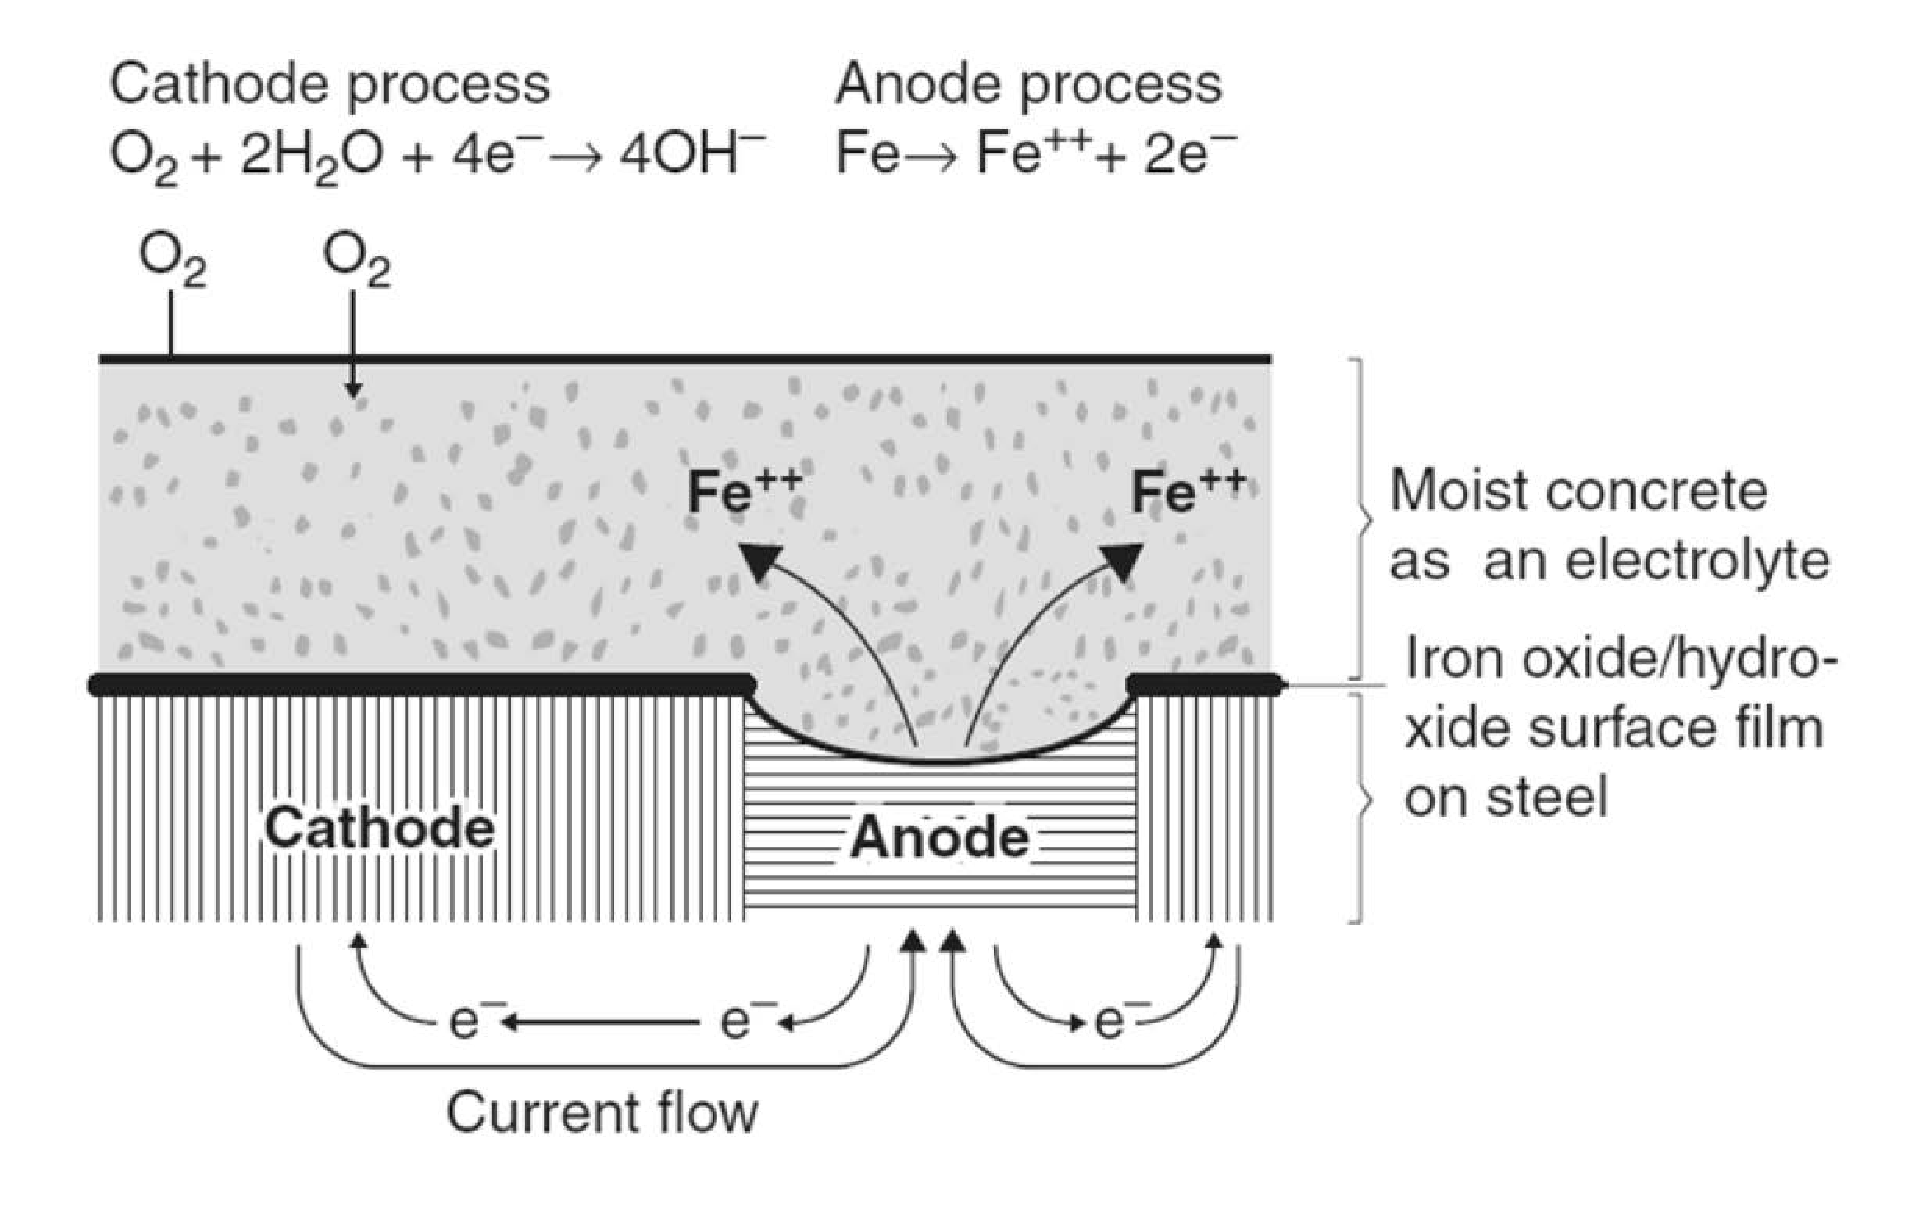
\includegraphics[width=0.9\textwidth]{Chapter-2/figs/Corrosion_Process}
\caption{Corrosion process in reinforcing steel bar \cite{Mehta2014}}
\label{fig:corr1}
\end{figure}

Corrosion plays an important role in the further deterioration of the seismic response of a structure. The parameters that describe corrosion are (1) Time to initiation of corrosion (Tcorr), (2) Corrosion growth in reinforcing steel, and (3) the mechanical properties of corroded reinforcing steel

\subsection{Time to corrosion}

 Jensen et al performed a series of experiments to measure the chloride ingress in the cement and mortar paste  \cite{Jensen1999}. In their study, it was determined that the ingress of chlorides follows Fick's law of diffusion, shown in \eref{eq:ficks_law}. Stewart et al solved \eref{eq:ficks_law}  in terms of the chloride ion concentration ($C(x,t)$), distance from concrete surface ($x$), time of exposure to chloride ions ($t$), and the chloride diffusion coefficient ($D_c$). The solution rendered equation \eref{eq.three} which describes the time to initiation of corrosion    \cite{Stewart1998}\cite{Y.Liu1998a}\cite{Thoft-Christensen}. Mean values for $C_0$ and $C_r$ have been previously defined for environments that are controlled by dicing salts \cite{Ghosh2010}\cite{Weyers1994}\cite{Enright1998}.

\begin{equation}
	\frac{\partial C(x,t)}{\partial t} = D_c \frac{\partial C(x,t)}{\partial x^2}
	\label{eq:ficks_law}
\end{equation}
\newline
\begin{equation}
  T_{corr}=\frac{x^2}{4 D_c} \left[erf^{-1} \left(\frac{C_0-C_{cr}}{C_0} \right) \right]^{-2}
  \label{eq.three}
\end{equation} 

\subsection{Rate of corrosion}

Vu et al developed an empirical model to evaluate the corrosion rate \cite{Vu2000}\cite{Stewart1998}. In their study a constant corrosion rate was assumed. However, it is known that the corrosion rate is not constant over time because it is dependent on factors such as the quality of concrete, the amount of oxygen available in the environment, and the relative humidity.  Nonetheless, for long term studies this approximation is valid. The underlying assumptions of this model are a relative humidity of 75\% and a temperature of 20°C. The model developed by Vu et al is shown in \eref{eq.CorrosionRate}. Figure \ref{fig:hist1} shows the corrosion rate for different concrete covers ($d_c$), as a function of the water to cement ratio ($w/c$). In general, for large values of cover depth the rate of corrosion decreases rapidly, and as the water to cement ratio (i.e. lower quality concrete) increases the rate of corrosion increases.

\begin{equation}
  i_{corr}=\frac{37.5(1-w/c)}{d_c}
  \label{eq.CorrosionRate}
\end{equation} 

\begin{figure}[htbp]
\centering
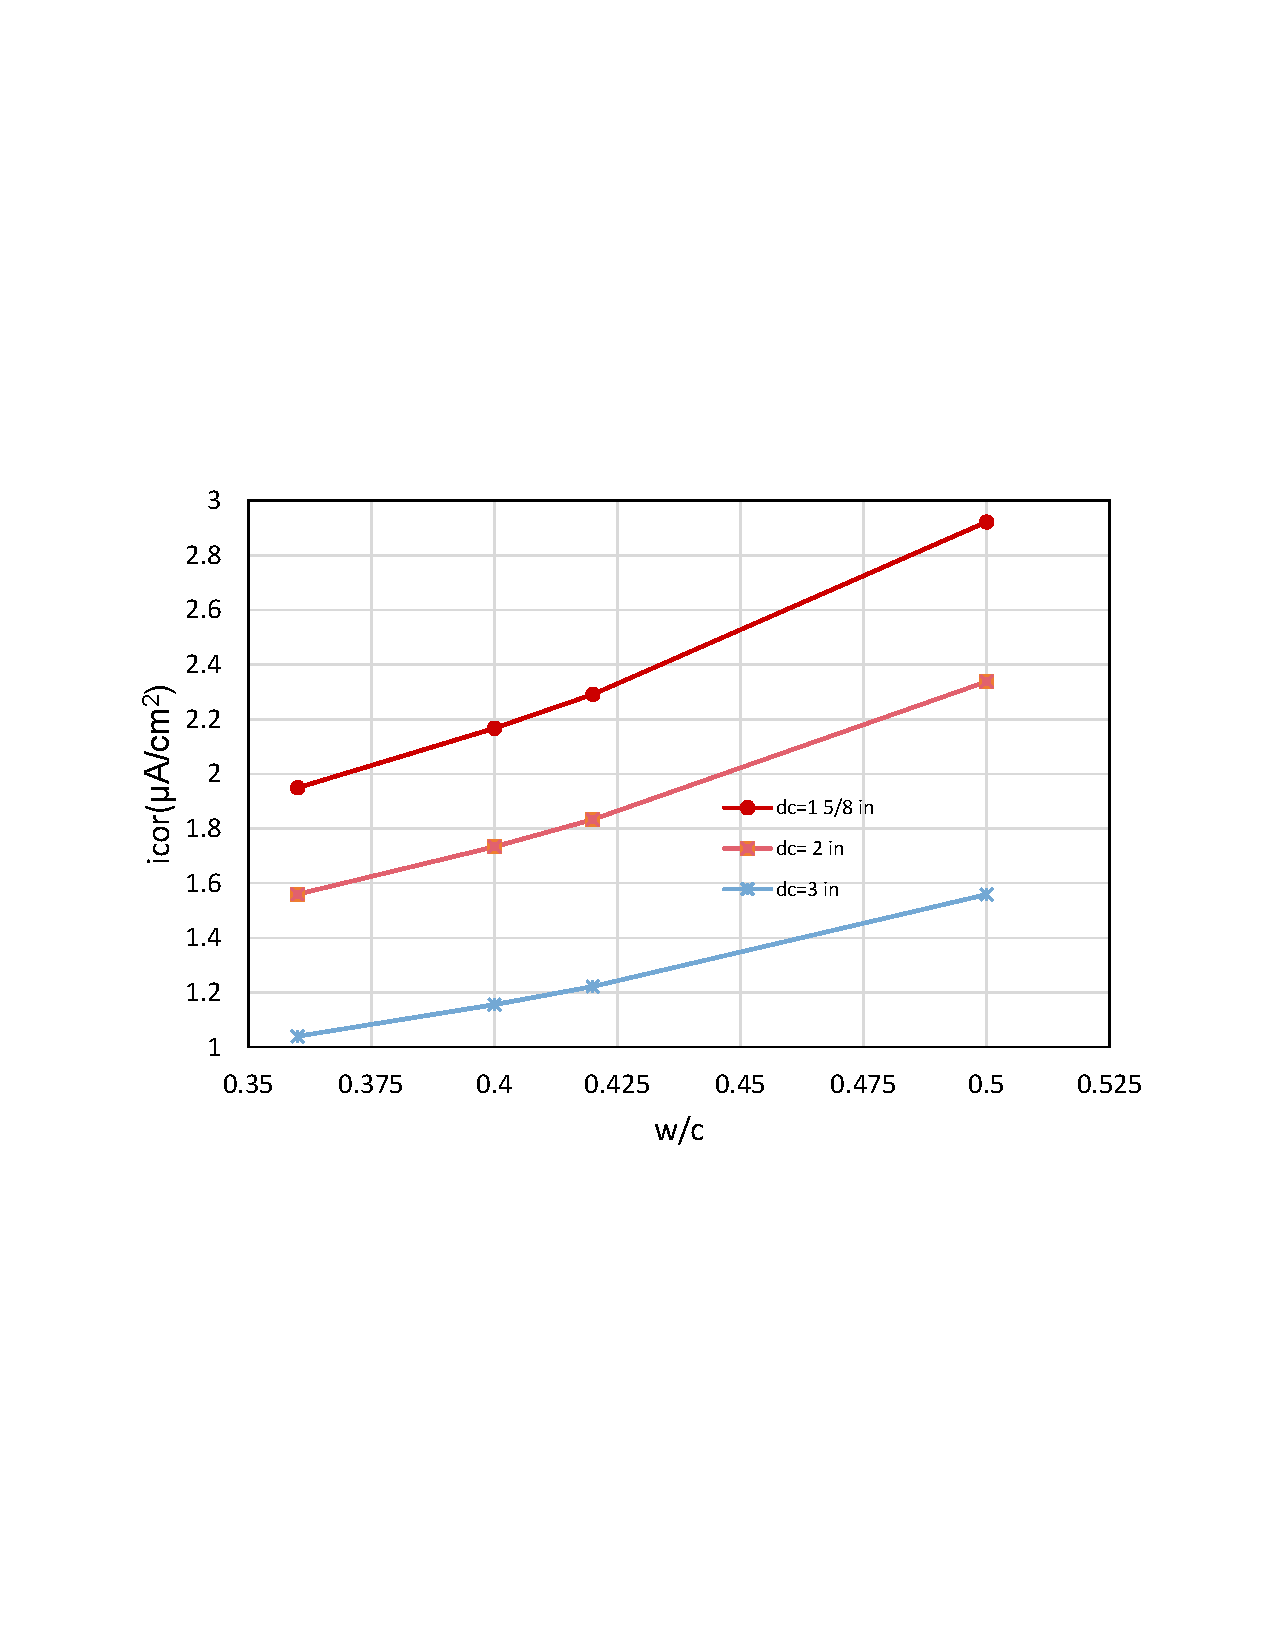
\includegraphics[width=0.85\textwidth]{Chapter-2/figs/wc_icor}
\caption{Concrete water to cement ratio vs rate of corrosion}
\label{fig:hist1}
\end{figure}

In addition, Vu et al  further improved the model of corrosion growth in reinforcing steel developed by Stewart et al \cite{Vu2000}\cite{Stewart1998}\cite{Choe2008}\cite{Ghosh2010}. Their proposed model describes the reduction in diameter of reinforcing steel ($d_{corr}(t)$ as a function of time described in \eref{eq.CorrosionEvolution}. Figure \ref{fig:DiameterEvolution} shows this model applied to a rebar with an initial diameter ($d_{bi}$) of 3/4 inch, a concrete cover of 1-1/2”, and water to cement ratios ranging from 0.36-0.50.

\begin{equation}
  d_{corr}(t)=d_{bi}-\frac{1.0508(1-w/c)}{d_c} (t-t_{corr})^{0.71}
  \label{eq.CorrosionEvolution}
\end{equation} 

\begin{figure}[htbp]
\centering
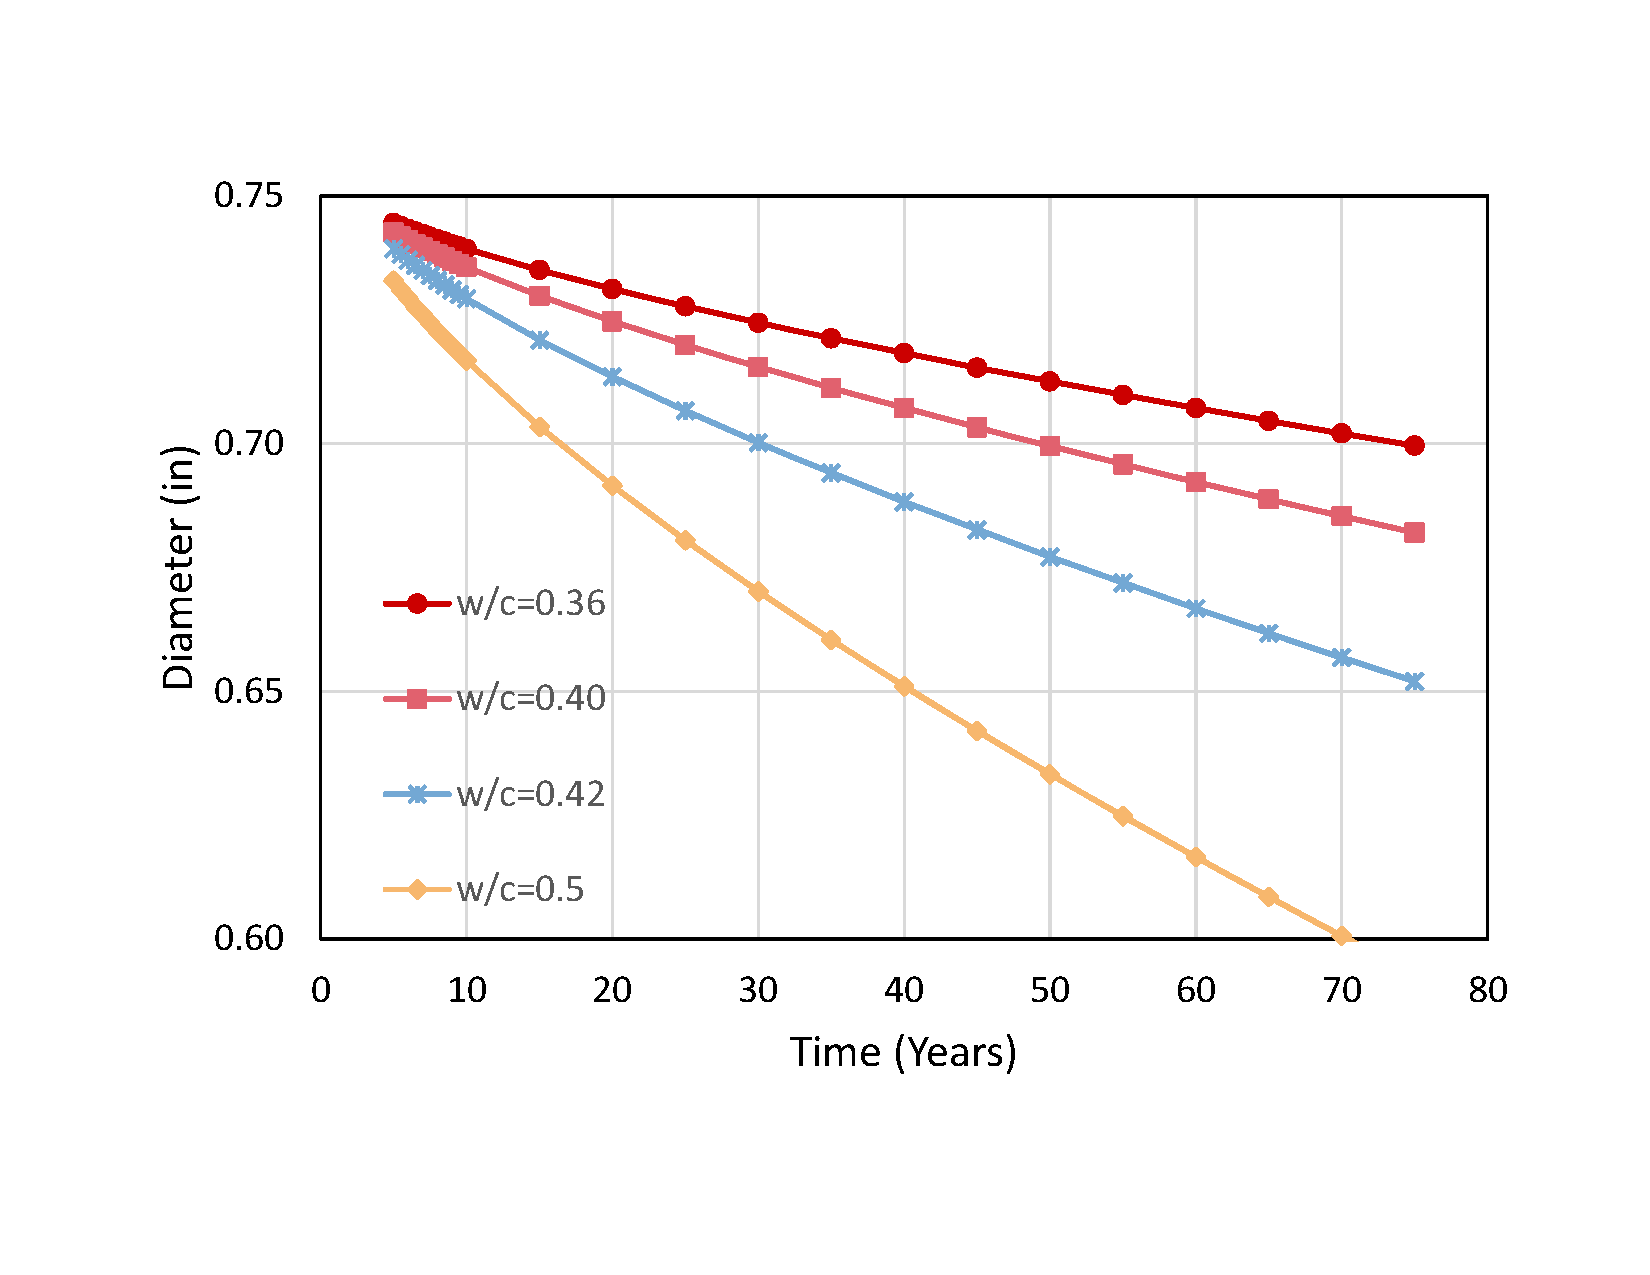
\includegraphics[width=0.85\textwidth]{Chapter-2/figs/DiameterDecrease}
\caption{Diameter decrease due to corrosion}
\label{fig:DiameterEvolution}
\end{figure}

Further, the evolution of corrosion in reinforcing steel can be expressed in the percent loss of mass of a rebar. If uniform corrosion is assumed, this can be expressed as the percent of reduction of diameter. The corrosion level can be expressed as shown in \eref{eq.CorrosionLevel}.

\begin{equation}
	CL=\frac{d_{i}-d(t)}{d_{i}}*100%
  \label{eq.CorrosionLevel}
\end{equation} 

Combining \eref{eq.CorrosionEvolution} with \eref{eq.CorrosionLevel},  the variation of the corrosion level can be described as a function of time. Figure  \ref{fig:CorrosionLevel_Time} shows the results of this process.

\begin{figure}[htbp]
\centering
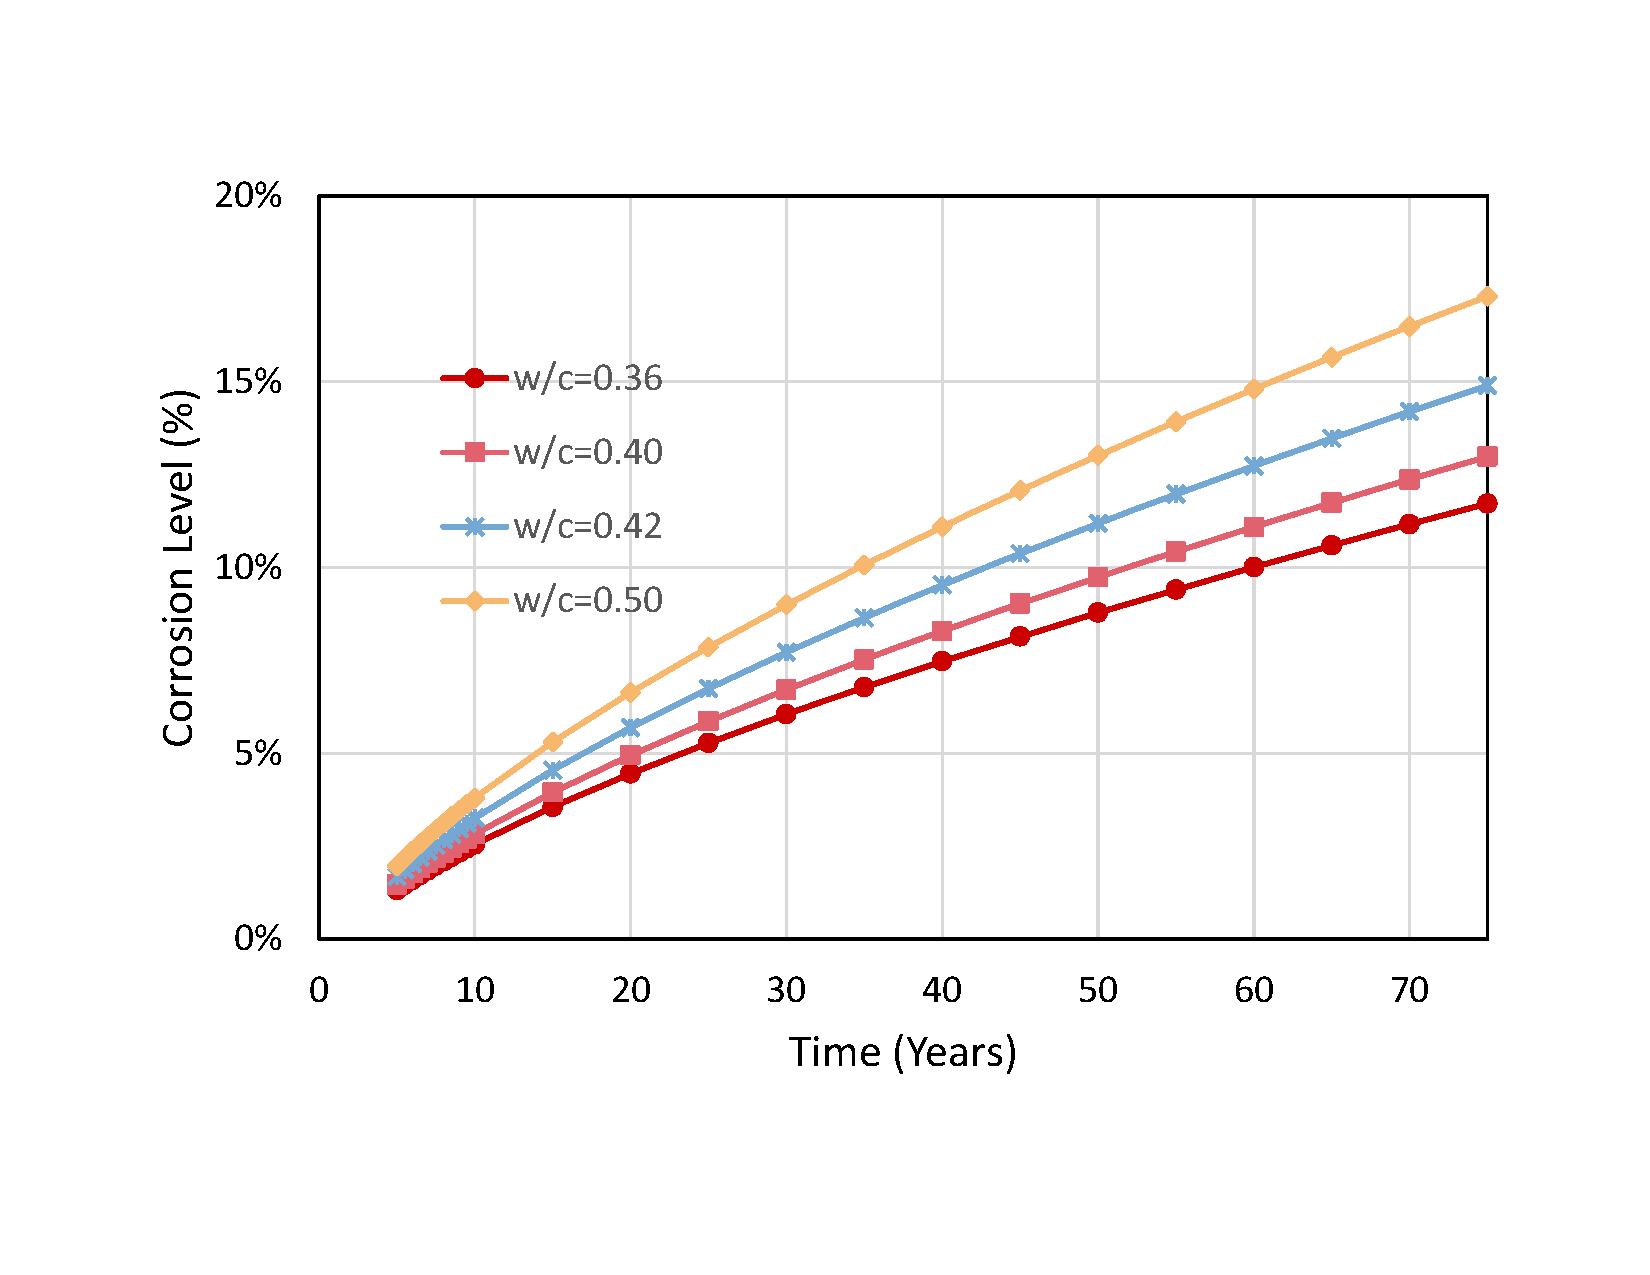
\includegraphics[width=0.85\textwidth]{Chapter-2/figs/CorrosionLevel}
\caption{Corrosion level vs time (years)}
\label{fig:CorrosionLevel_Time}
\end{figure}

\subsection{Corrosion modified properties of reinforcing steel bars}

Yuan et al \cite{Yuan2017a} performed tension tests on corroded rebars and determined that the mechanical properties of steel change with the level of corrosion. In general, as corrosion increases, the yield strength and ultimate strength of the reinforcing steel decrease.  The variation of the mechanical properties is shown in \eref{eq.eleven} for the yield strength and ultimate strength of the reinforcing steel.

\begin{equation}
  f_{y,C}=f_{yo}(1-0.021C)
  \label{eq.eleven}
\end{equation} 
\[
  f_{u,C}=f_{yo}(1.018-0.019C)
\]

One of the limitations in their study is that the accelerated corrosion process used to develop the corrosion in the rebars did not account for the depassivation process that naturally occurs in rebars embedded in concrete. Chapter \ref{chap-three} shows a proposed experimental assessment that will provide an accurate evaluation of the mechanical properties of corroded reinforcing steel. 

\section{Steel strain aging}

\subsection{Metallurgical process}

It is generally accepted that strain aging is due to the diffusion of carbon and/or nitrogen atoms in solution to dislocations that have been generated by plastic deformation. Initially, an atmosphere of carbon and nitrogen atoms is formed along the length of a dislocation, immobilizing it. Extended aging, however, results in sufficient carbon and nitrogen atoms for precipitates to form along the length of the dislocation\cite{Overby2017}\cite{Hosseini2015}.

These precipitates impede the motion of subsequent dislocations and result in some hardening and loss in ductility. The extent of strain aging, which is a thermally activated process, depends primarily on aging time and temperature. In general, extended aging results in a saturation value above which further aging has no effect \cite{Restrepo-Posada1994}.

A second strengthening mechanism occurs when cold deformation (alone) is applied to steels. When dislocations break away from their pinning interstitial atoms and begin the movement causing slip they begin to intersect with each other. A complex series of interactions between the dislocations occurs, causing them to pin each other, decreasing their mobility. The decreased mobility also results in higher strength, lower ductility and lower toughness. As a result, cold deformed steels already have lowered ductility and toughness before any strain aging occurs. When heating follows cold deformation, the loss in ductility and toughness is greater. It is this combination of events that is the most damaging to the toughness of structural steels \cite{Momtahan2009}.

\subsection{Strain aging effects in structures}

Strain aging is the process by which steel after being subjected to large strains, develops an increased strength and reduced ductility with time. Large earthquakes can cause this effect on structures built with mild steel. Therefore, it is  important to include strain aging in a time dependent analysis. Furthermore, strain aging will cause an increase in the strength of the plastic hinge and as a consequence plastic hinges may form in regions of the structures that have not been designed for such demands. The effects of strain aging may also alter the transverse reinforcement due to cold bending, making them susceptible to brittle failure\cite{Momtahan2009}.

According to Restrepo-Posada\cite{Restrepo-Posada1994}, most strain aging occurs in the first 37 days. In addition, Momtahan et al  \cite{Momtahan2009} studied strain aging effects with respect to time at different levels of pre-strains. The pre-strains ranged from $2\varepsilon_y $ to $10\varepsilon_y$, for a time frame of 3 days to 50 days. Their results determined that a significant effect of strain aging took place from pre-strains $5\varepsilon_y$ and on. Strains higher than $15\varepsilon_y$ indicate a performance level in which substantial damage has been induced in the structure such that it is deemed unrepairable and therefore pre-strains higher that $15\varepsilon_y$ are impractical and were not studied \cite{Momtahan2009}.

Momtahan et al correlated the increase in yield strength as a function of time and the pre-strain in reinforcing steel bars. The proposed equations are shown below:

For $10\varepsilon_y$

\begin{equation}
  \frac{f_y}{f_{yi}}=0.0026t+0.9838
  \label{eq.twelve}
\end{equation} 

For $5\varepsilon_y$

\begin{equation}
  \frac{f_y}{f_{yi}}=0.0008t+0.996
  \label{eq.thirteen}
\end{equation} 

For $2\varepsilon_y$

\begin{equation}
  \frac{f_y}{f_{yi}}=0.0004t+0.9979
  \label{eq.fourteen}
\end{equation} 

It is proposed to limit the increase in yield strength obtained at 50 days, which was the limit of scope of their study. Equations \ref{eq.twelve} to  \ref{eq.fourteen} are plotted in \fref{fig:hist4}

\begin{figure}[htbp]
\centering
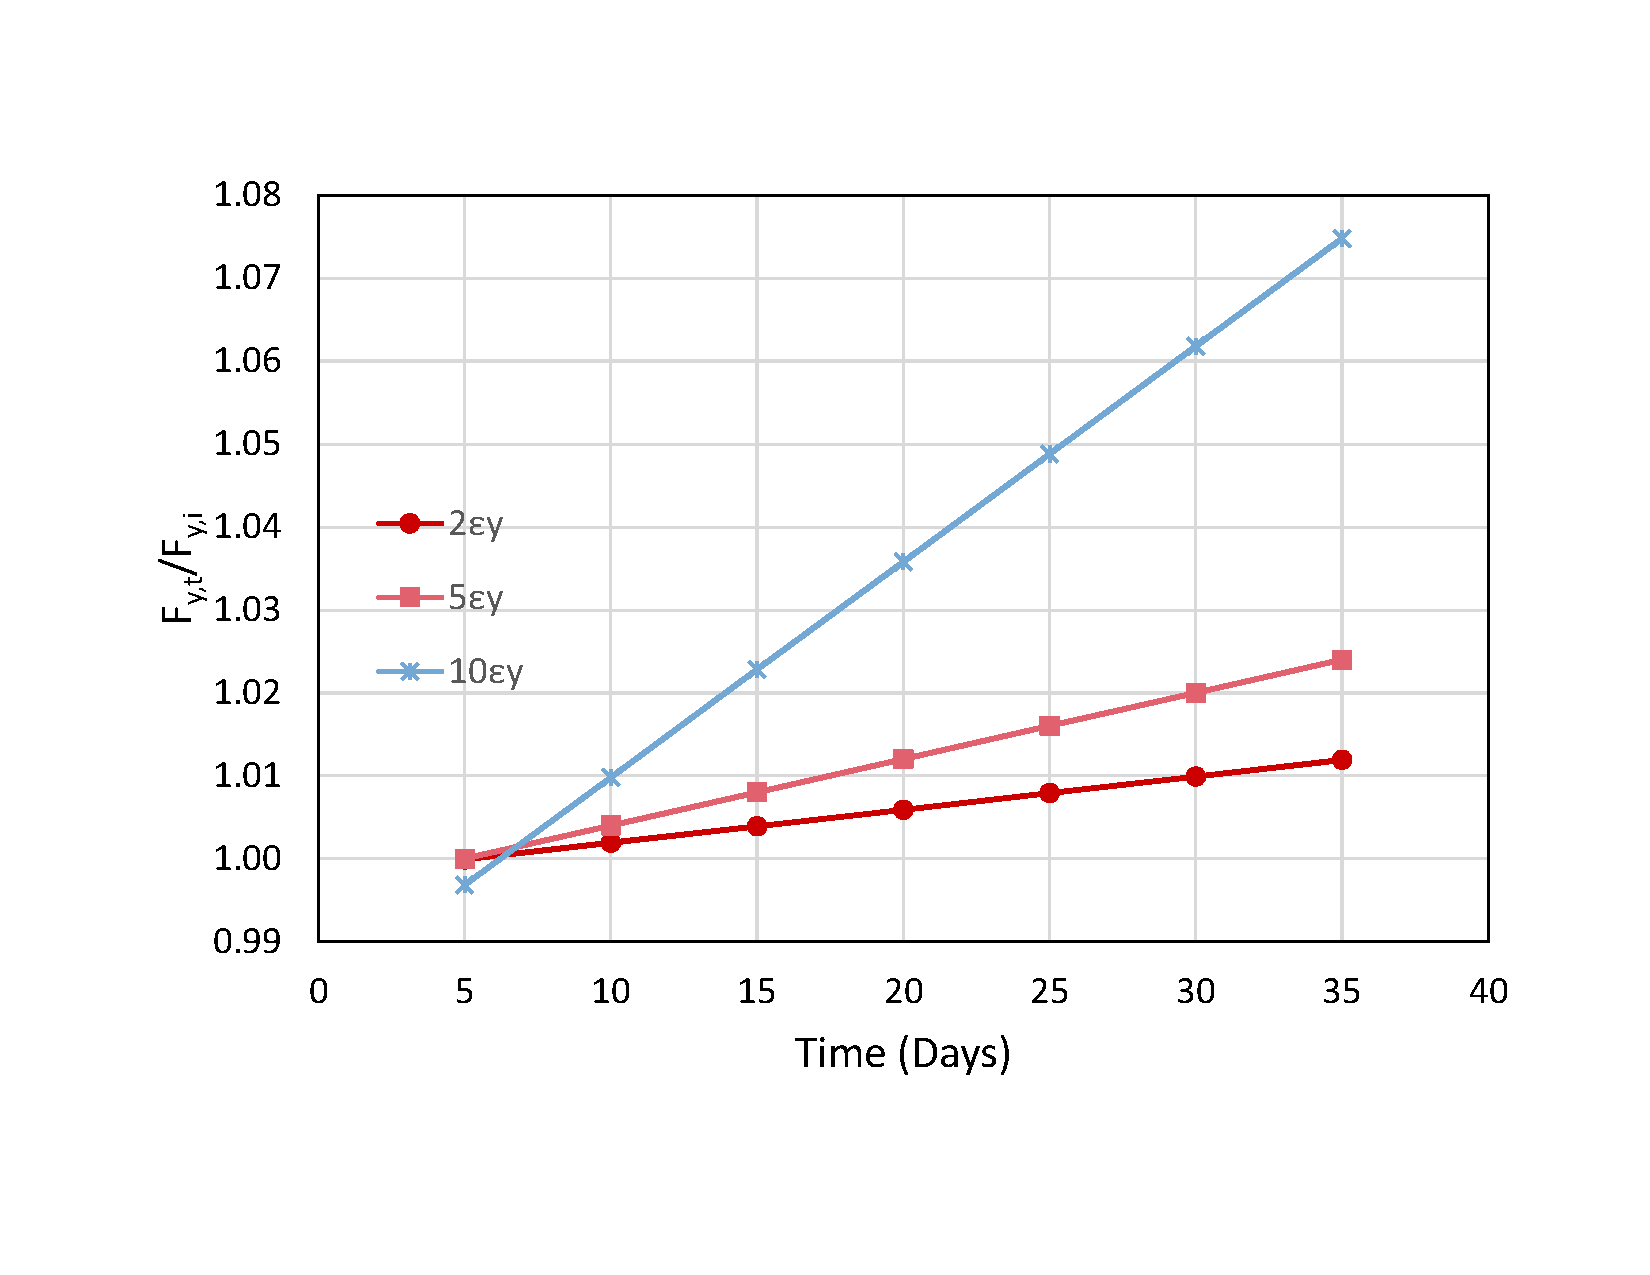
\includegraphics[width=0.7\textwidth]{Chapter-2/figs/StrainAging_TimeDependent}
\caption{Strain aging effect on yield strength vs time (days)}
\label{fig:hist4}
\end{figure}

\section{Damage Indexes}
The effect of cumulative damage in structures was studied by Park and Ang (1985) \cite{Young-JiPark1985} in their study the authors proposed the damage index as shown in \eref{eq.DamageIndex}. The damage index was used as a measure to quantify damage in terms of the maximum experienced earthquake and the absorbed hysteretic energy.

\begin{equation}
  D=\frac{\Delta_{m}}{\Delta_{u}}-\beta \frac{E_h}{F_{y}\Delta{u}}
  \label{eq.DamageIndex}
\end{equation} 

$\Delta_{m}$: Maximum deformation under earthquake

$\Delta_{u}$: Ultimate deformation under monotonic loading

$F_{y}$: Calculated yield strength

$E_{h}$: Total hysteretic energy

$\beta$: Dimensionless constant 

\begin{figure}[htbp]
\centering
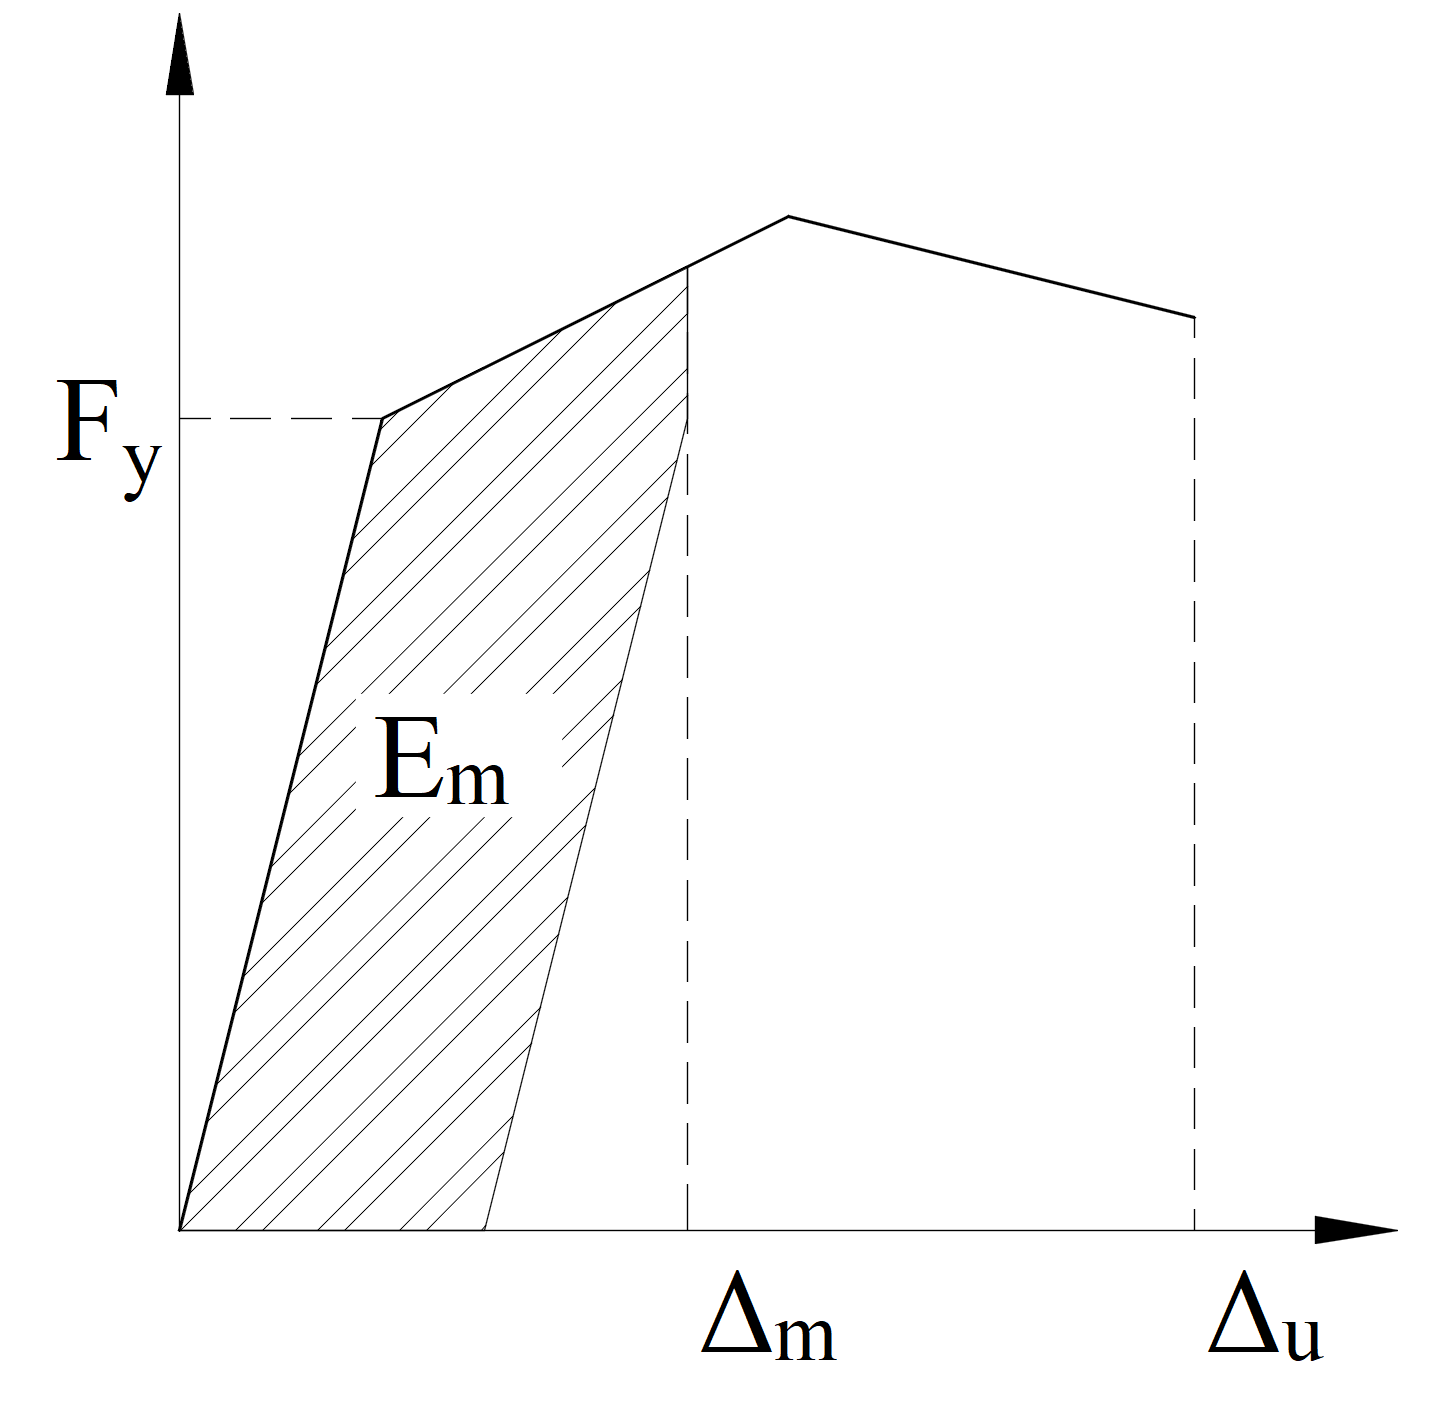
\includegraphics[width=0.6\textwidth]{Chapter-2/figs/Park_and_Ang_Model}
\caption{Park and Ang conceptual scheme}
\label{fig:Paa}
\end{figure}

Equation \ref{eq.DamageIndex} was derived for concrete elements. The first term here is a simple, pseudo-static displacement measure. The second term accounts for cumulative damage. This concept is shown in \fref{fig:Paa}. The advantages of this model are its simplicity and flexibility in adapting the model to correlate with experimental data.  

However, this model has several limitations. Firstly, the calibration of the $\beta$ coefficient with observed damage has proven to be very low ($\beta=0.05-0.15$) \cite{Young-JiPark1985} \cite{Ghosh2015}, rendering the second term relatively inconsequential compared to the contribution of the first term. A sample result is taken from Gosh et al \cite{Ghosh2015}, which applied a modified version of the Park and Ang damage index in terms of the moment ($M_{y}$), the rotation ($\theta_y$), and curvature ductility ($\mu$). The modified model is expressed in \eref{eq.DamageIndexGhosh}.

\begin{equation}
	D=\frac{\mu_{m}}{\mu_{u}}-\beta\frac{E_h}{M_{y}\theta_y\mu{u}}
	\label{eq.DamageIndexGhosh}
\end{equation}

Using the following values: $\mu_{m}=4.93$; $\mu_{u}=17.02$; $M_{y}=8751.375$; $\theta_y=0.0042$; $E_{h}=119.07$; $\beta=0.05$ 

And substituting in equation \eref{eq.DamageIndexGhosh}:
\[
 D=\frac{\mu_{m}}{\mu_{u}}-\beta\frac{E_h}{M_{y}\theta_y\mu{u}}=0.3
	\]
\textbf{First term}:
\[
\frac{\mu_{m}}{\mu_{u}}=\frac{4.93}{17.02}=0.2897
\]
\textbf{Second term}: 
\[	
	\beta \frac{E_h}{M_{y}\theta_y\mu{u}}=0.05\frac{119.07}{8751.375*0.0042*17.02}=0.0103
\]

It can be seen that 97\% of the damage index comes from the first term, which is the elastic term, and the inelastic part is only 3\% of the total. 

Despite its limitations, several studies have used or modified this model to study the effects of cumulative damage for different structures. Those of relevant importance are those performed by Kunnath et al \cite{Kunnath1992}, who used a modified Park and Ang model, to account for damage at the local level for elements in the structural analysis program IDARC 3.0. In this software, for the case of multiple degrees of freedom buildings they also added parameters to consider the damage at the inter-story level and the global model. Ghosh et al \cite{Ghosh2015} developed a damage accumulation framework to estimate the probability of exceeding a damage index for multiple ground motions. Other regressions have been proposed \cite{Khashaee}, \cite{Fajfar1992}, \cite{Roufaiel} but show no improvement in assessing the damage state of a structure. While these studies provide an insight into some of the characteristics of damage accumulation they, still rely on the Park and Ang model and therefore carry the same limitations.

Krawinkler (1987) \cite{Krawinkler1987} proposed a method that considered damage as a function of low cycle fatigue parameters. The form of the Krawinkler damage index for steel components, weldments, and local buckling has a general shape of the Miner model. This model relies on the accumulation of plastic deformations. While this model has proven to work well for the evaluation of individual steel structure elements, it does not provide a way to generalize damage for other types of structures.


\section{Multiple earthquake loading}

The evaluation of multiple seismic events has been scarcely studied; however, their effects have been felt in numerous earthquake sequences such as the Christchurch 2010, Umbria-Marche Earthquake 1997 and the Puerto Rico Earthquakes 2020. The hypothesis is that accumulation of damage will restart in a smaller seismic event to achieve a prescribed limit state, similar to how corrosion and other aging phenomena might impact the intensity needed to achieve a future limit state. 

In the literature the study of multiple earthquake loading can be classified in two groups:

\begin{itemize}
	\item Mainshock-aftershock sequences
	\item Mainshock sequences
\end{itemize}

These studies have shown what are some of the effects of multiple earthquake loading for different structures.

\subsection{Mainshock-aftershock sequences loading }

Strong aftershocks can increase the state of damage of a building or even collapse an already damaged structure. It is therefore important to quantify the increase of seismic demands in structures due to aftershock loading. In recent years different studies have been carried out to develop methodologies that consider these effects.

Tesfamariam et al \cite{Tesfamariam2015} investigated the increase in the demands for multiple degrees of freedom systems (MDOF). Their study carried out a parametric study of RC frame buildings and RC frame with infill masonry buildings. A series of mainshock-aftershock sequences were applied. Their results showed that there is an increase of 10\% in the interstory drift demands for the RC frame structures. The authors did not check for strain limit states, and therefore a damage limit state may have been reached. Thus, their study might have underestimated the structural performance. Similarly Raghunandan et al \cite{Raghunandan2015} studied the vulnerability of RC frame structure. Their study showed that depending on the level of interstory drift achieved during the mainshock the additional damage experienced during the aftershock will be different. For example, the authors showed that for an RC frame that experiences 4\% or more interstory drift in the mainshock, the median capacity to resist aftershock shaking is reduced by about 40\%. Furthermore, other studies have focused on the behavior of single degree of freedom (SDOF) systems response to mainshock-aftershock (MS-AS) sequences \cite{Hatzigeorgiou2009}\cite{Manafpour2019}. Hatzigeorgiou et al focused on determining the inelastic displacement coefficient variation due to the MS-AS sequence. Their study concluded that there is an increase in the inelastic displacement demands, however, the limitations in their study did not report what occurs to the performance limit states. Further, Manafpour et al studied the seismic drift behavior of structures to MS-AS sequences for far-field earthquakes and near-field earthquakes. Their study concluded that for SDOF structures near-field earthquake sequences were the most damaging, increasing the drifts by as much as 45\%.

Researchers have applied two earthquake selection procedures for mainshock-aftershock sequences. The first method incremental dynamic analysis (IDA), consists of 1)subjecting the nonlinear building model to a ground motion having a particular intensity, 2) recording the response of the structure \cite{Vamvatsikos2002}, 3)in successive analyses, the ground motion is incrementally scaled to a higher intensity measure (IM), and 4)the structural response is recorded in each analysis. The IDA procedure was extrapolated to generate MS-AS sequence as follows: 1)Apply the IDA to the mainshocks to obtain different levels of damage in the structure, 2) after each mainshock include an incrementally scaled aftershock, and 3)Change the polarity of the aftershock, which refers to the direction of the aftershock variation to the mainshock. \fref{fig:MS-AS_Luco} shows one of the resulting MS-AS sequences using the IDA methodology. Due to the use of scaling factors the IDA methodology uses artificial mainshock-aftershock sequences. In addition, the IDA analysis can be computationally expensive. For instance, the authors reported a total of 9900 ground motion sequences per structure.

\begin{figure}[htbp]
\centering
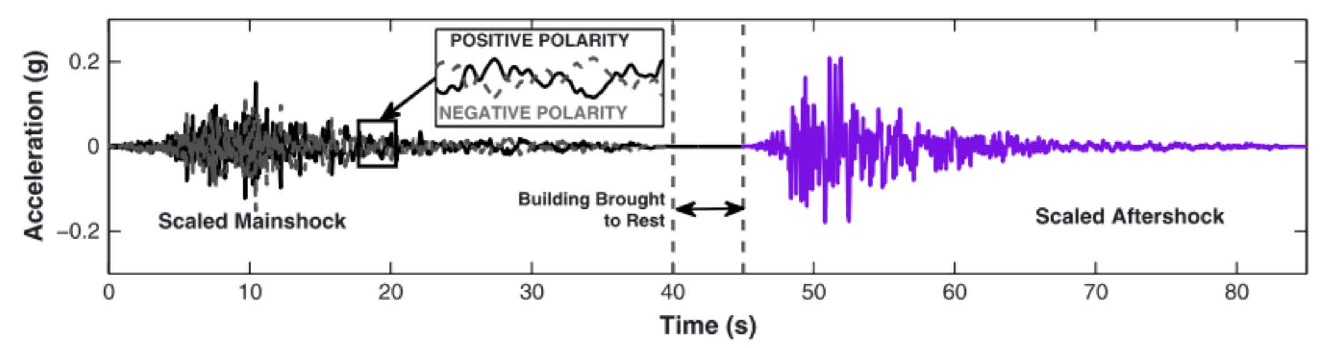
\includegraphics[width=0.6\textwidth]{Chapter-2/figs/MS-AS_sequence_Luco}
\caption{Mainshock-aftershock sequence train of ground motions \cite{Raghunandan2015}}
\label{fig:MS-AS_Luco}
\end{figure}

The second method consists in matching the MS-AS sequences to a site seismic hazard curve obtained from a probabilistic seismic hazard analysis (PSHA). Tesfamariam \cite{Tesfamariam2015} used conditional mean spectra (CMS) to match and select mainshock-aftershock sequences for structures located in Vancouver, BC. Their study selected MS-AS sequences from two databases of ground motions, NGA-West2 \citep{Ancheta2014}, and the K-NET//KiK-net \cite{NIEDK-NETKiK-net2019}. The CMS process consists of computing the expected response spectrum associated with a target spectral acceleration ($Sa$) value at a single period, using the known values from PSHA such as the magnitude, distance, and $\epsilon$ values. In their study the authors used CMS to select the MS-AS sequences for different earthquake scenarios a)Crustal earthquake, b) Interface, and c) Inslab. They hypothesized that different earthquake regimes would have different MS-AS sequence characteristics such as higher $Sa$ values at low periods for interface earthquakes or high values for crustal earthquakes. \fref{fig:MS-AS_Goda} shows this selection for a structure with a 0.4s period for crustal earthquakes. The CMS method adapts to the site conditions, no scaling of MS-AS is required since the selection is optimized to ground motion sequences stored in the databases. Since the CMS method uses site-specific data, it can be a part of an analytical framework that can be adapted to different seismic regions.

\begin{figure}[htbp]
\centering
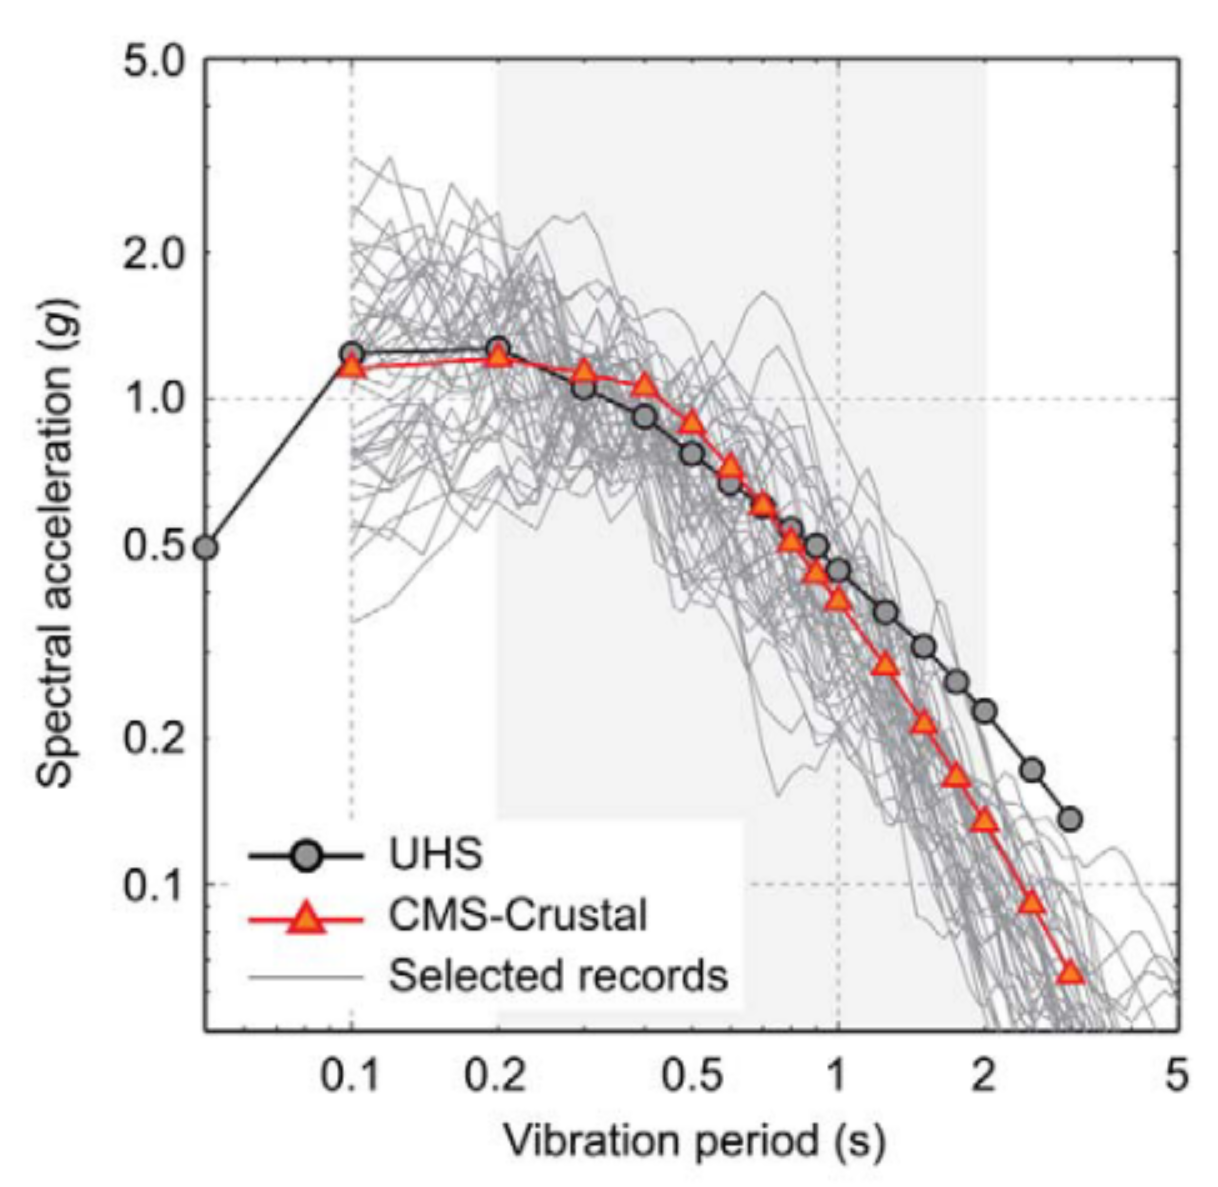
\includegraphics[width=0.5\textwidth]{Chapter-2/figs/CMS-Tesfamariam_MS-AS_seq}
\caption{Mainshock-aftershock sequence selection at T=0.4s for crustal earthquakes in Vancouver, British Columbia \cite{Tesfamariam2015}}
\label{fig:MS-AS_Goda}
\end{figure}

\subsection{Mainshock sequences loading}

Reliable prediction of earthquakes is currently impossible on any time scale.  However, for a large region, earthquakes recurrence time can be modeled reasonably well as a Poisson process. Sunasaka \cite{Sunasaka1993} developed mainshock sequences that followed a Poisson process. Their study focused on the accumulation of damage due to mainshock sequences, and mainshocks-aftershocks sequences. Damage accumulation was accounted for by the Park and Ang index. The authors used ground motion prediction equations to develop artificial mainshock sequences. Their study calculated the recurrence period, magnitude, location and peak ground acceleration for each of the mainshocks. The author subjected an SDOF bridge in Eureka, CA to the mainshock sequence shown in   \fref{fig:MS-MS_Sunasaka}. While the results shows a significant increase in the damage index due to mainshock sequences, the conclusions are limited by the assumption that a Poisson process can be applied to single faults, which has not shown good correlation with observed events\cite{Shearer2009}. While this study shows what could be possible if mainshocks were predictable in small regions, more advances in seismology are needed to confidently apply the proposed methodology.

\begin{figure}[htbp]
\centering
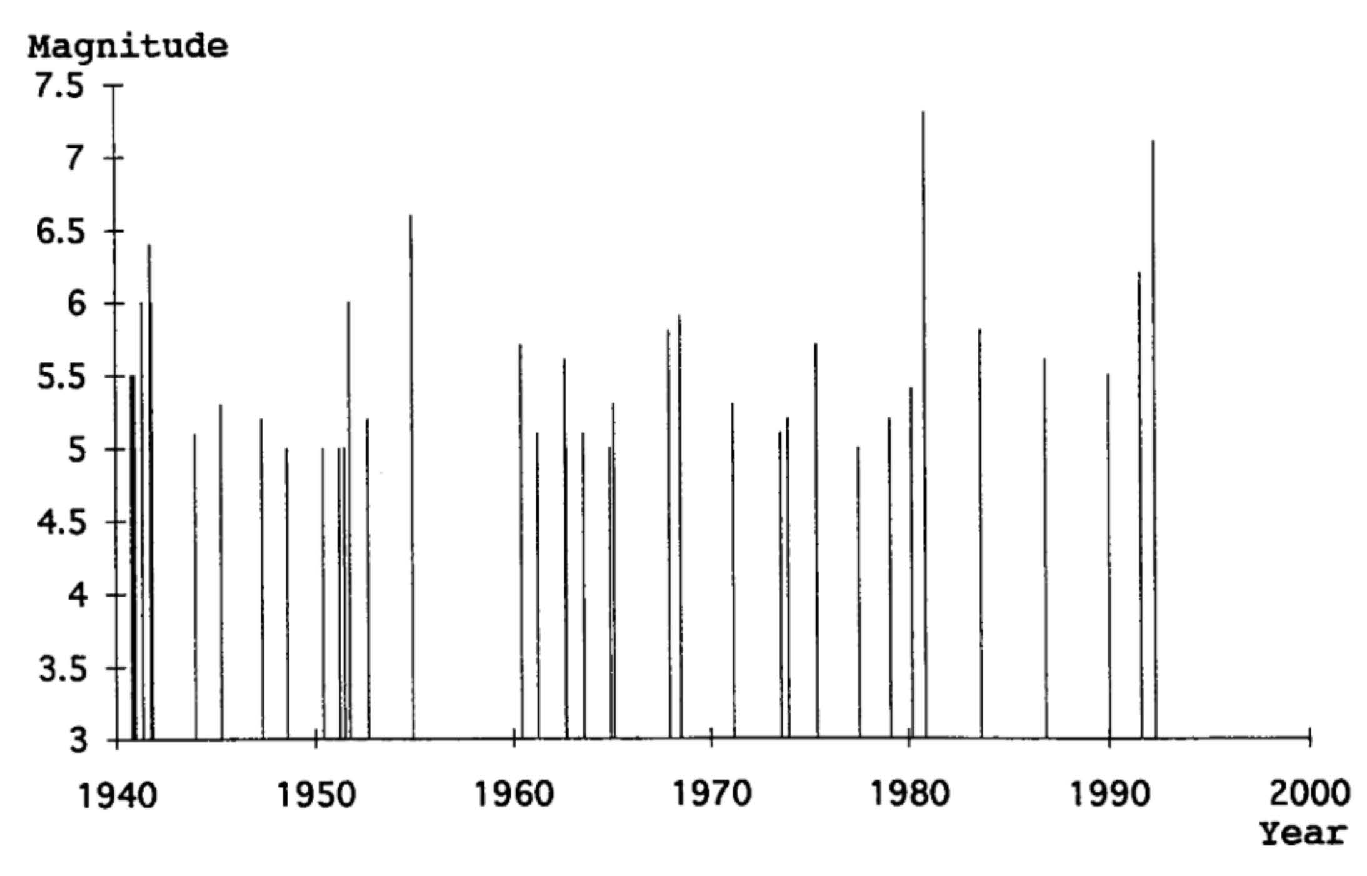
\includegraphics[width=0.5\textwidth]{Chapter-2/figs/Mainshock_sequence_01}
\caption{Mainshock sequence selection at Eureka, CA \cite{Sunasaka1993}}
\label{fig:MS-MS_Sunasaka}
\end{figure}

Other studies have used three equally spaced mainshocks \cite{Hatzigeorgiou2009}. The three equally spaced mainshocks can be deployed without much computational effort, however, there is not a seismological basis for the use of three equally spaced mainshocks. Therefore, the use of this methodology would be limited to a scenario analysis and not useful for analysis and analysis, since the probabilities of three equally spaced in time mainshocks on any given structure is very low.

\section{Aging of structures}

There have been attempts by many researchers to establish the best way to characterize the aging of structures.

In recent years studies have focused on the effect of cumulative damage. These studies have focused on assessing the damage accumulation under different loading conditions such as multiple earthquakes, corrosion and life span of the structure. Two main approaches to tackle this field of study have been observed:

\begin{itemize}
	\item Probabilistic framework
	\item Fragility curves
\end{itemize}

\textbf{Probabilistic Framework}

One of the most widely used probabilistic frameworks is the Pacific Earthquake Engineering Research Center (PEER) Performance Based Design (PBD). PEER PBD can be expressed by the following equation:
\begin{equation}
\nu_{DM}(dm^{LS})=\iint D_{DM|EDP}(dm|edp)|,dG_{EDP|IM}(edp|im)||\,d\nu_{IM}(im)|
\end{equation}

Mackie et al \cite{Mackie2007} using  the PEER PBD, developed the performance based damage design (PBDD) and performance based loss design (PBLD) by defining the probabilistic demand, damage, and loss model parameters in terms of reinforced concrete column damage. The RC column damage was defined in terms of drift ratios limit states of concrete spalling, bar buckling and failure. 

The authors show that for a given intensity measure (IM) and a confidence level of achieving a limit state, it is possible to then define the probability  of exceeding that limit state.

While this methodology was able to define damage and incorporate it into the PEER PBD framework, the authors did not consider  strain to define the limit states. In addition, a recent study by Krish et al has shown that other intensity measures such as spectral displacement at effective first mode period ($S_{d}(T_{1})$) provide a better intensity measure \cite{Krish2018}.

\textbf{Fragility Curves}

Another common trend in this subject is the use of fragility curves to estimate the effect of damage in structures. Two main approaches were found in the literature. One of them relied on the Park and Ang Model damage index to define damage, while the second approach related damage to drift.

Ghosh et al \cite{Ghosh2015} formulated a damage accumulation framework. Their study relied on the Park and Ang Damage index explained in the previous section. The study performed a series of nonlinear time history analyses for two cases:

\begin{itemize}
	\item Using a constant main shock hazard occurrence rate (3 main shocks in a 50-year period)
	\item Mainshock - Aftershock series using a time-dependent aftershock hazard occurrence rate
\end{itemize}

Evaluation of the damage index exceeding probability for the two cases was performed. The results from their study showed regression equations that statistically predict the damage index as a function of earthquake intensity and damage history. This study revealed that for both mainshock and aftershock scenarios there was a significant increase in the probability of damage index exceeding under repeated shock scenarios. While this study shows the importance of considering damage accumulation, these results have to be taken with caution, since they present the same disadvantages as the Park and Ang damage index.

Ghosh et al \cite{Ghosh2010} also studied the effects of corrosion on time dependent seismic fragility curves. Their study characterizes corrosion in concrete columns as a continuous phenomenon that occurs as a function of time. The authors also considered the effects of corrosion on steel bridge bearings. The authors then ran a series of NLTHA analyses for different aging times of the structures. Based on their analysis, time dependent fragility curves were presented. The results showed that as time increases, and corrosion increases as a consequence, the probability of exceeding a limit state increases. In their study, limit states were defined on the basis of inter-story drifts which were obtained from experimental results and field observations \cite{Padgett2007}. It is important to mention that the limit states used in their study were not defined on the basis of strains or other structural property. Instead the limit states came from a survey performed in central and southeastern United States departments of transportation, on the premise of a range of experienced inter-story drifts and the time taken to repair them. In addition, assuming that corrosion is a continuous process has to be cautiously taken as valid. This is because site information such as temperature, water to cement ratio, the addition of cementitious materials such as silica fume, and the environment (e.g. coastal vs inland) affect the rate of propagation of corrosion\cite{Thoft-Christensen}.

While these studies provide a general view on how damage increases the likelihood of observing collapse or deterioration of the seismic performance, the methods used to arrive at those conclusions can be misleading since the definition of damage as either a Damage Index or Drift are not the best parameters to quantify the damage. It is our belief that strain-based limit states will provide a better understanding of the implications of damage accumulation.

\section{Research Gap}

Many studies have tried to show the importance of quantifying the effects of accumulated damage and multiple shocks throughout the lifetime of a structure.  Therefore, it is important to develop a model that establishes the likelihood of achieving a limit state as the structure ages. In addition,  it is important to understand the impacts of aging on bridge seismic performance. Furthermore, bridges in seismic areas can be subjected to main shock and aftershocks. Therefore, a methodology that incorporates both aging and multiple seismic events is needed.

Damage accumulation is a topic that has been gaining momentum in the engineering community, this study will better inform  the potential future conditions of a structure to stakeholders such as state DOTs, building owners, and practicing engineers. In the literature it was observed that damage accumulation has been studied using the Park and Ang damage index or drift-based limit states to measure damage accumulation. Different researchers have also included corrosion into their scope of analysis, which shows that aging conditions play an important role in the deterioration of a structure. In addition, Krish \cite{Krish2018} determined that spectral displacement at first effective period is an improved intensity measure (IM), while the past literature used the peak ground acceleration (PGA) as the controlling IM. This research will develop a parametric study using a series of single degree of freedom (SDOF) systems, subjecting them to different conditions such as corrosion, steel strain aging and strength aging. The SDOF structures will be subjected to a sweep of ground motions using nonlinear time history analysis to obtain maximum strain demands. With the results from NLTHA, fragility functions will be used to show the increase in the likelihood of reaching a performance limit state due to aging of the structure. In addition, this research will provide the engineering community with a design framework to account for damage accumulation in their analysis and guide decisions on the resiliency of a structure. In addition, this study will provide a methodology in which the Direct Displacement-Based Design (DDBD) is modified to consider the effects of damage and aging conditions.

\subsection{General Objectives}
The main goal of this research is to provide a design methodology to consider damage for performance based seismic design of structures. In addition, this study will demonstrate the implications of aging conditions and multiple earthquakes for the design of bridge RC columns.

\subsection{Specific Objectives}
\begin{itemize}
	\item Incorporate different aging conditions and develop fragility curves that considers strain limit states as a measure of damage
	\item Establish limit states for corroded rebars
	\item Inform the research community of the necessary methodology to appropriately mimic real corrosion process in material experiments of corroded rebars, which can later be extrapolated to large scale testing of RC columns subjected to corrosion
	\item Consider the effects of multiple earthquakes for  two cases: (1) Mainshock-Aftershock sequence, and (2) Mainshock-Aftershock sequence with the effects of time between the mainshock and the aftershock.
	\item Incorporate these results into the Direct Displacement Based Design (DDBD) methodology, through the use of factors that correspond to the aging conditions
\end{itemize}
\chapter{Experimental phase: mechanical properties and performance of corroded reinforcing steel}
\label{chap-three}

Corrosion is the main aging condition that affects structures, therfore, the success of this study relies on the most accurate representation of the corrosion process. As mentioned in Chapter 2 previous studies developed accelerated corrosion specimens with high current densities and did not account for the passivation of the reinforcing steel. Therefore, a main component of this study is to obtain reliable mechanical properties of the corroded reinforcing steel. To achieve this the experimental process is divided in to three main processes, (1) generate the passive layer in rebar specimens, (2) depassivate and corrode the rebar specimens (3) obtain the mechanical properties of the reinforcing steel by performing tension tests and buckled bar tension tests. It is expected that this careful process will mimic as best as possible the real aging conditions of rebars inside the concrete mix environment. This chapter outlines the rebar preparation, experimental setup, instrumentation, and expected results.
%The experimental portion of this research program consists of a total of 54 buckled bar tension tests using the method proposed by Barcley et al \cite{Barcley2019}.The experimental phase of this research aims at studtying the effects of depassivation in the modified mechanical properties of corroded grade 80 reinforcing steel, and the modification on the bending strain in corroded buckled bars. 

\section{Proposed experimental campaign}

It is known that the steel inside concrete generates a protective film due to the alkaline environment generated by the cement paste. The most common form of corrosion occurs via chloride attacks. During a chloride attack, the chloride in salts contacts the surface of the steel, this initiates the elimination of the protective film in a process known as depassivation. The proposed experimental campaign aims at simulating the process of corrosion as it would occur in a rebar embedded in concrete. The experiment process is outlined here:

\begin{enumerate}
	\item Passivation of the reinforcing steel
	\item Accelerated corrosion  of reinforcing steel
	\item Tension tests
	\item Buckled bar tension (BBT) test
\end{enumerate}

\textbf{Passivation of the reinforcing steel}

In order to simulate the conditions of rebars embedded in concrete, it is necessary to generate the passive layer on the surface of the reinforcing steel. There are two ways of generating the passive layer on the reinforcing steel, (1) embed rebars in concrete and wait for the passive layer to generate, (2) submerge the reinforcing steel in a synthetic pore solution that mimics the cement paste environment. The second option is more suited for material testing since it does not involve any form of demolishing. Ghods et al \cite{Ghods2010} developed different ten pore solutions to generate the passive film on the reinforcing steel surface. It is known that the cement paste has ions of $Ca^{+2}$, $Na^{+}$, $K^{+}$, and $(SO_{4})^{+}$. Therefore out of the ten pore solutions proposed by Ghods et al, five had this ions. Further, the authors presented a comparison on the quality of the passive fil, the film that was shown to have the best quality while having all the ions was selected for this study. The pore solution that is going to be deployed has the following concentrations:

\begin{itemize}
	\item Saturated calcium hydroxide $Ca(OH)_2$
	\item Sodium hydroxide $Na(OH)$ (4.00 g/l)
	\item Potassium hydroxide $(KOH)$ (11.22 g/l)
	\item Calcium sulfate dihydrate $Ca(SO)_4 + 2H_2O$ (13.77 g/l)
\end{itemize}

Since it is important to mimic real life applications, the rebars will be placed in the pore solution as received without any special surface preparation in the area of study. It has been shown that any form of special surface preparation affects the quality of the passive layer . Ghods et al showed that it takes a minimum of 8 to 13 days to generate the passive layer \cite{Ghods2009}, therefore the rebars will be placed in the pore solution for a minimum of 13 days. Figure \fref{fig:RebarPassivation} shows. 

In addition, it is necessary to protect the areas of the rebar that are going to function as grips for the rebars during the tension and BBT tests. Therefore the ends of the rebars will be protected with three different layers of protection. First a layer of two-part epoxy is placed, then a layer of electroplater tape and the third and final layer is shrink tube. This three layers ensure minimal corrosion in the grip areas of the rebar. Figures \fref{fig:RebarSpecimenGeomtry} and \fref{fig:RebarEndsProtection} show the specimen geometry and the preparation of the ends of the rebars.

\begin{figure}[htbp]
	\centering
	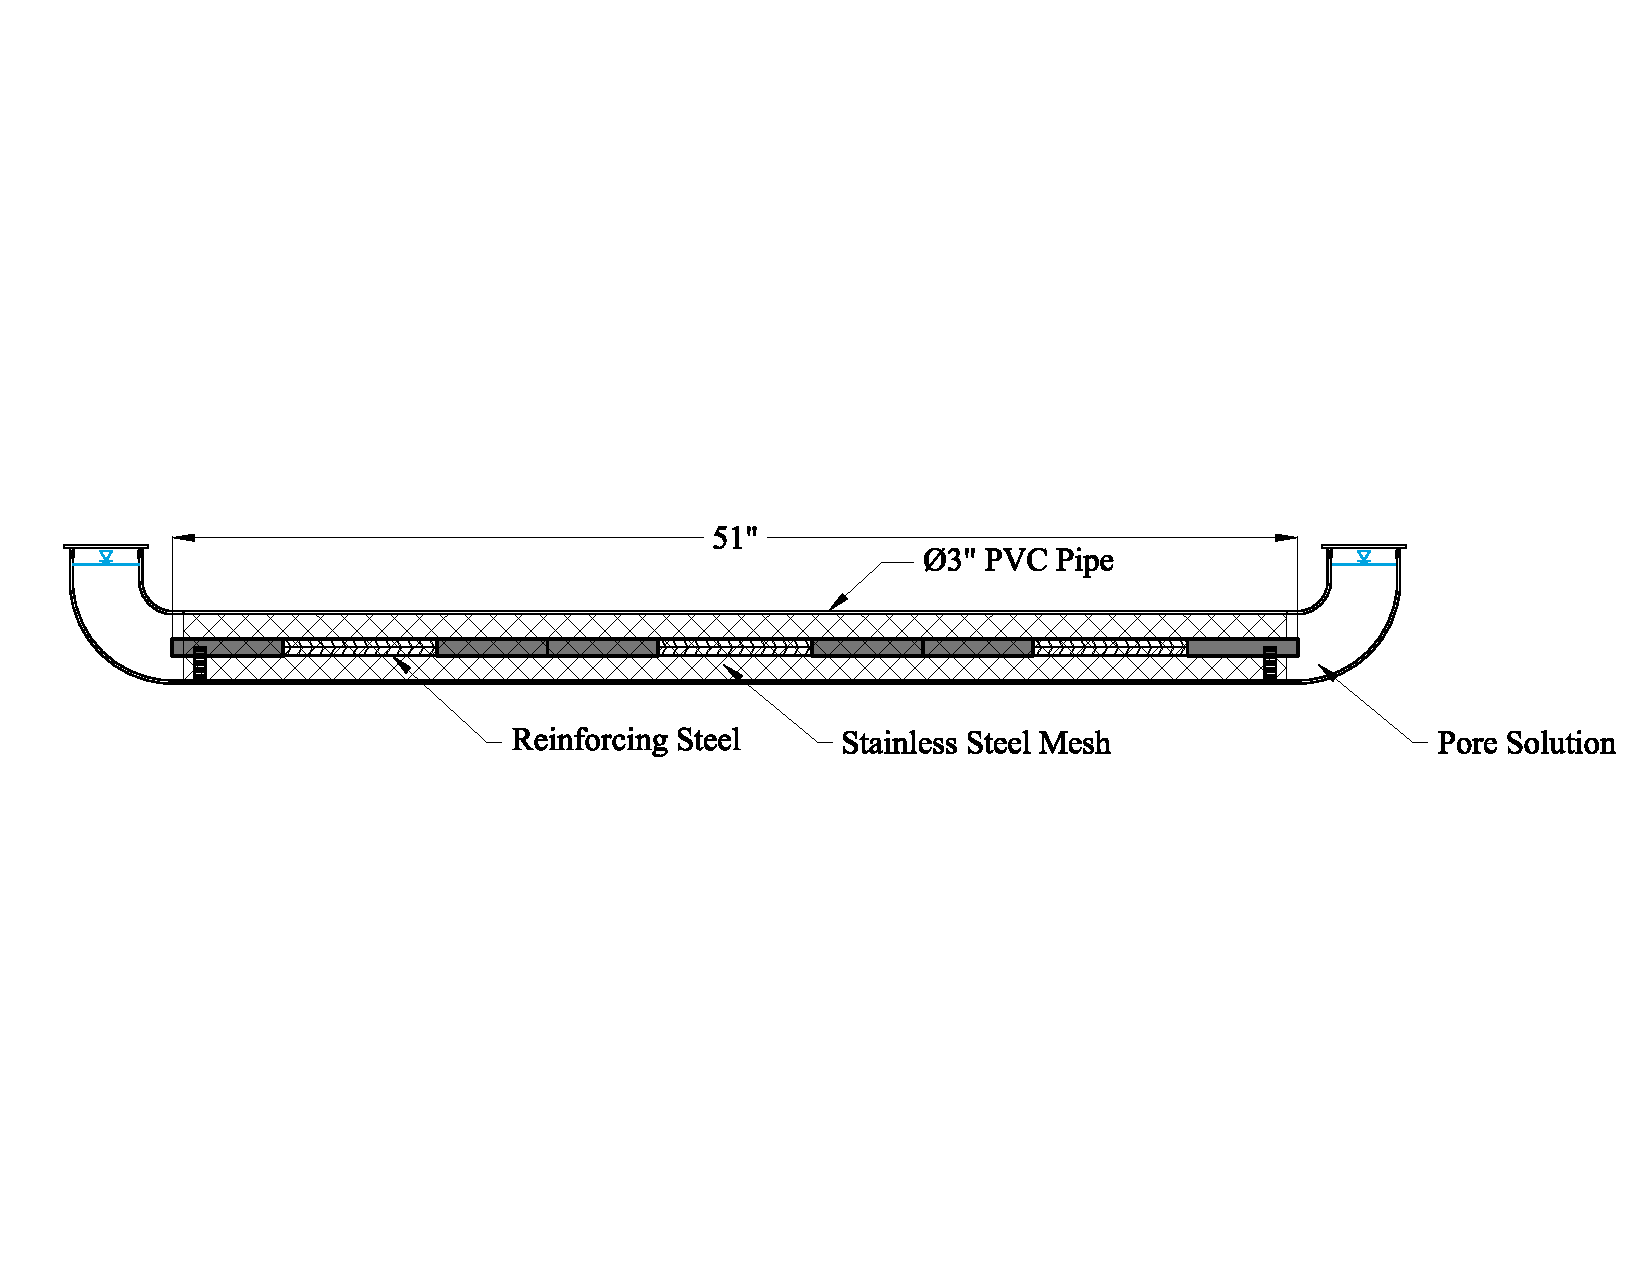
\includegraphics[width=1.0\textwidth]{Chapter-3/figs/AnodicPolarization_01}
	\caption{Rebars Passivation Process in Calcium Hydroxyde Pore Solution}
	\label{fig:RebarPassivation}
\end{figure}

\begin{figure}[htbp]
	\centering
	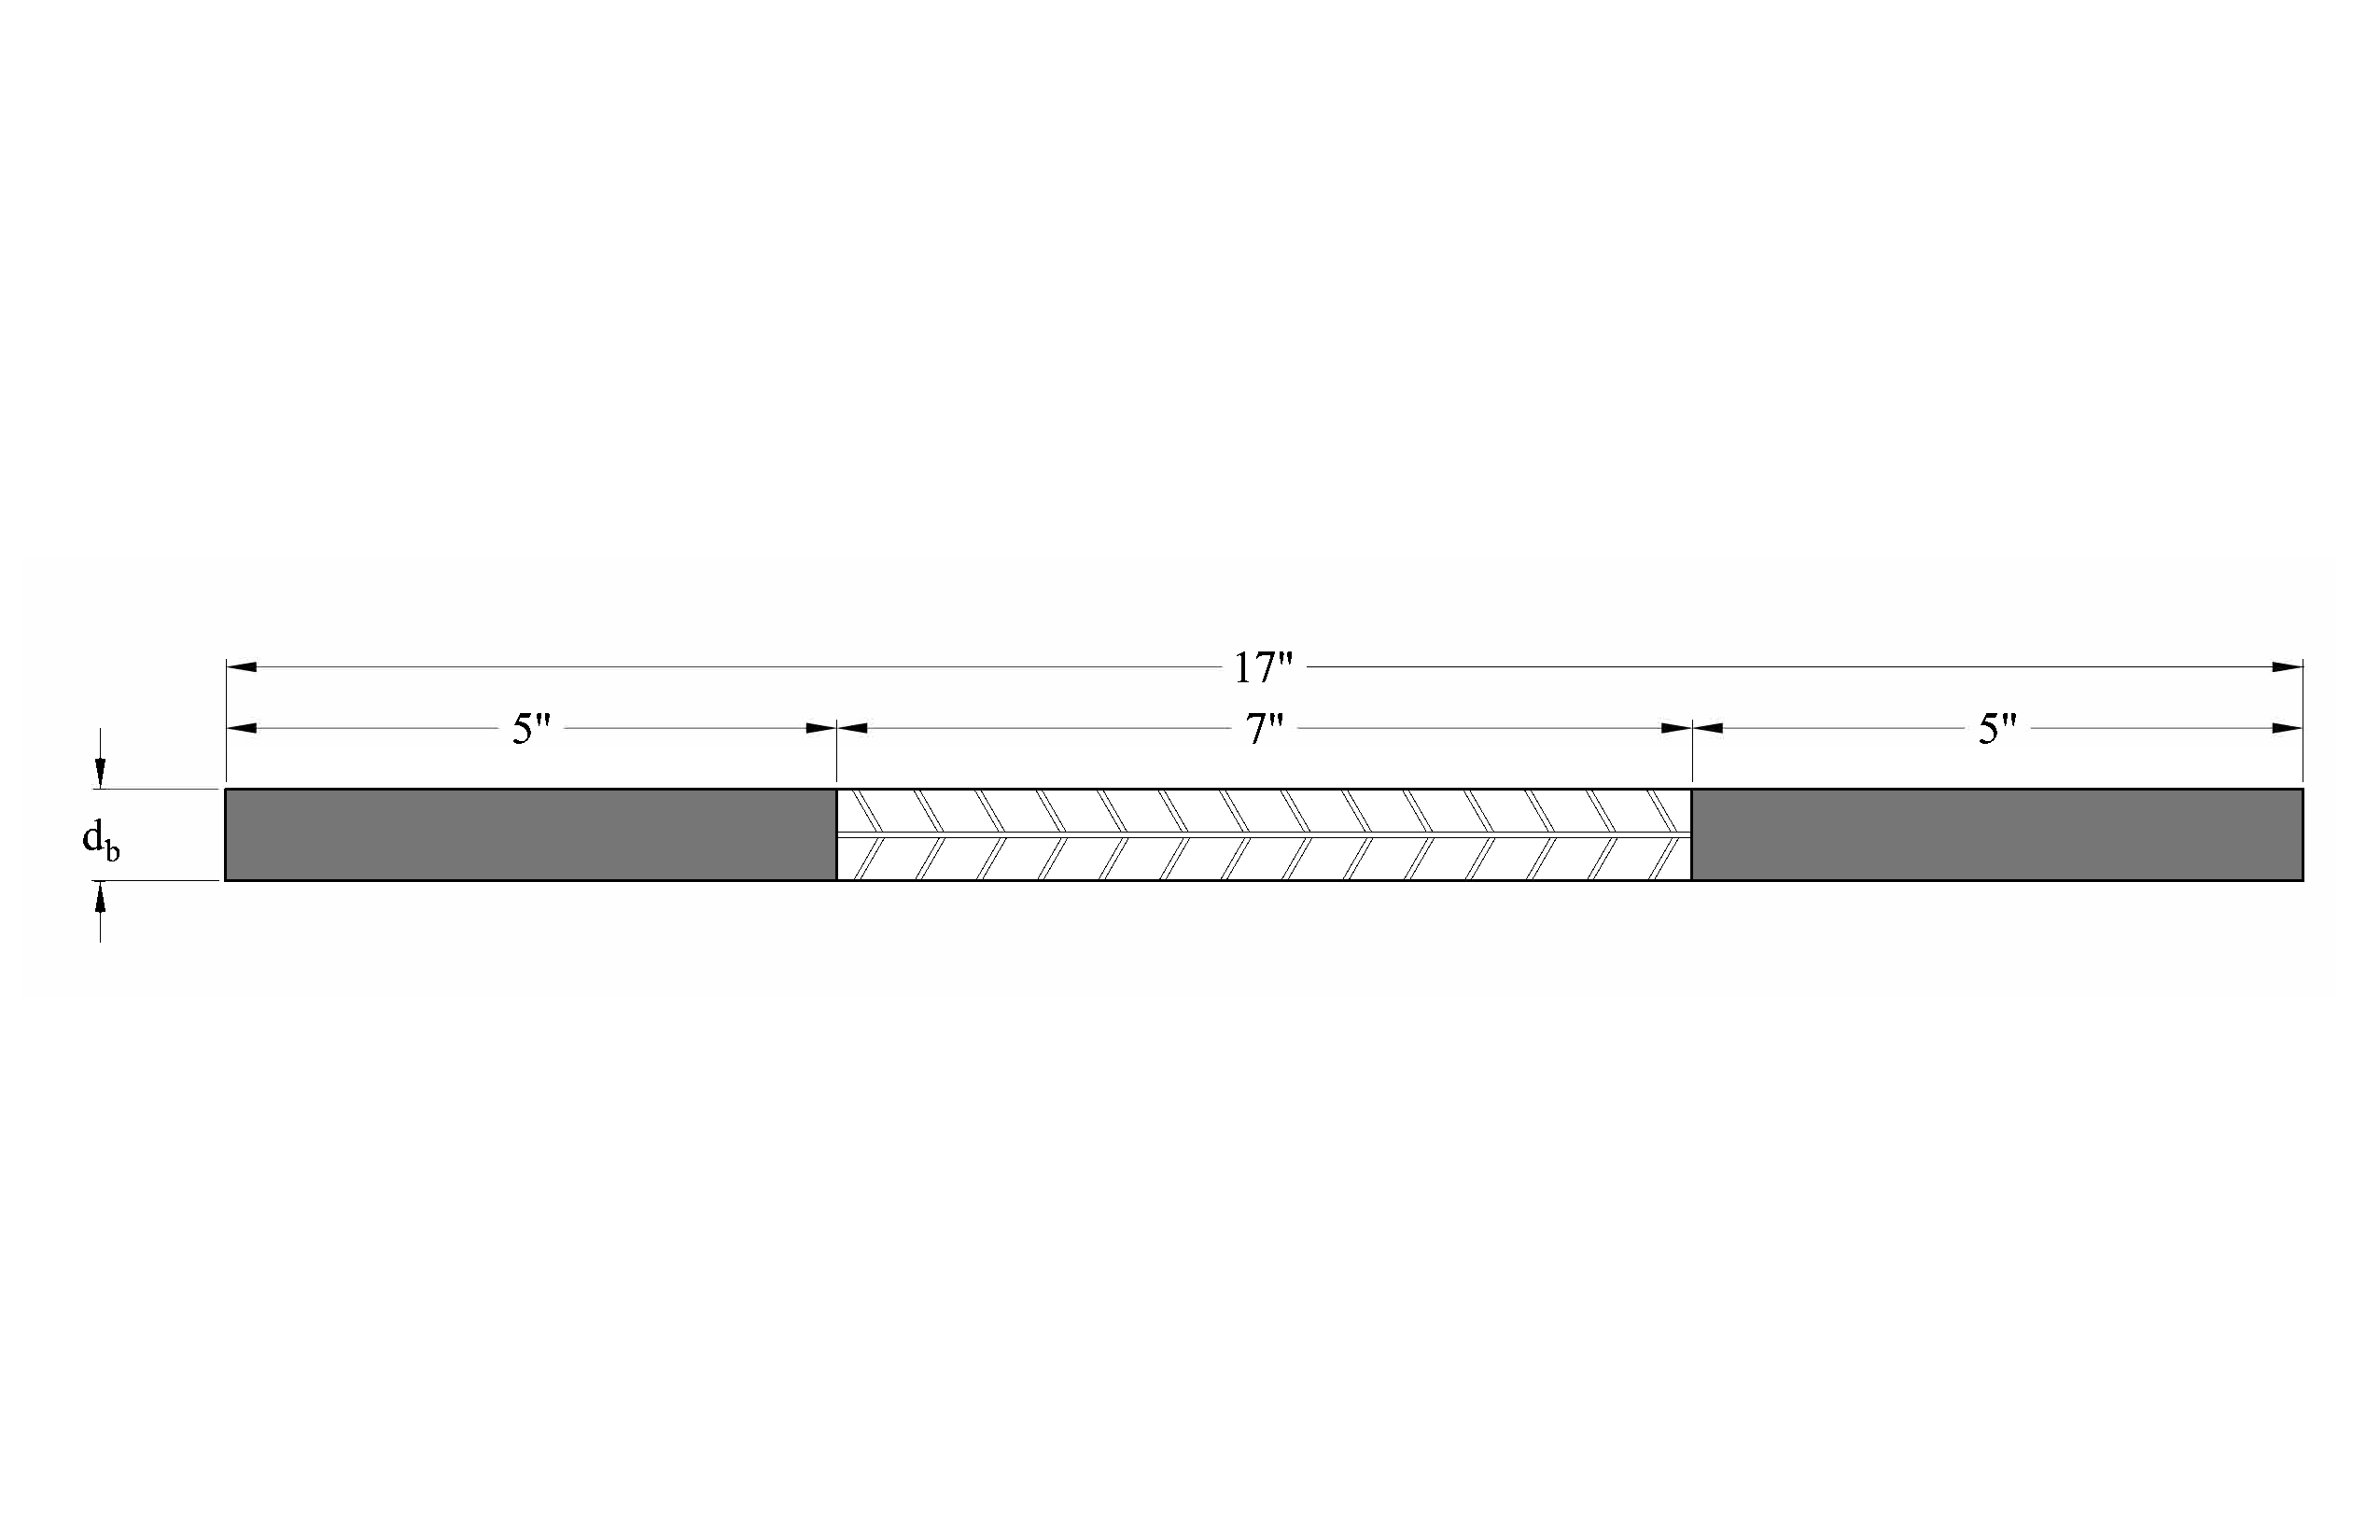
\includegraphics[width=0.9\textwidth]{Chapter-3/figs/RebarSamples}
	\caption{Rebar Specimen Geometry}
	\label{fig:RebarSpecimenGeomtry}
\end{figure}

\begin{figure}[htbp]
	\centering
	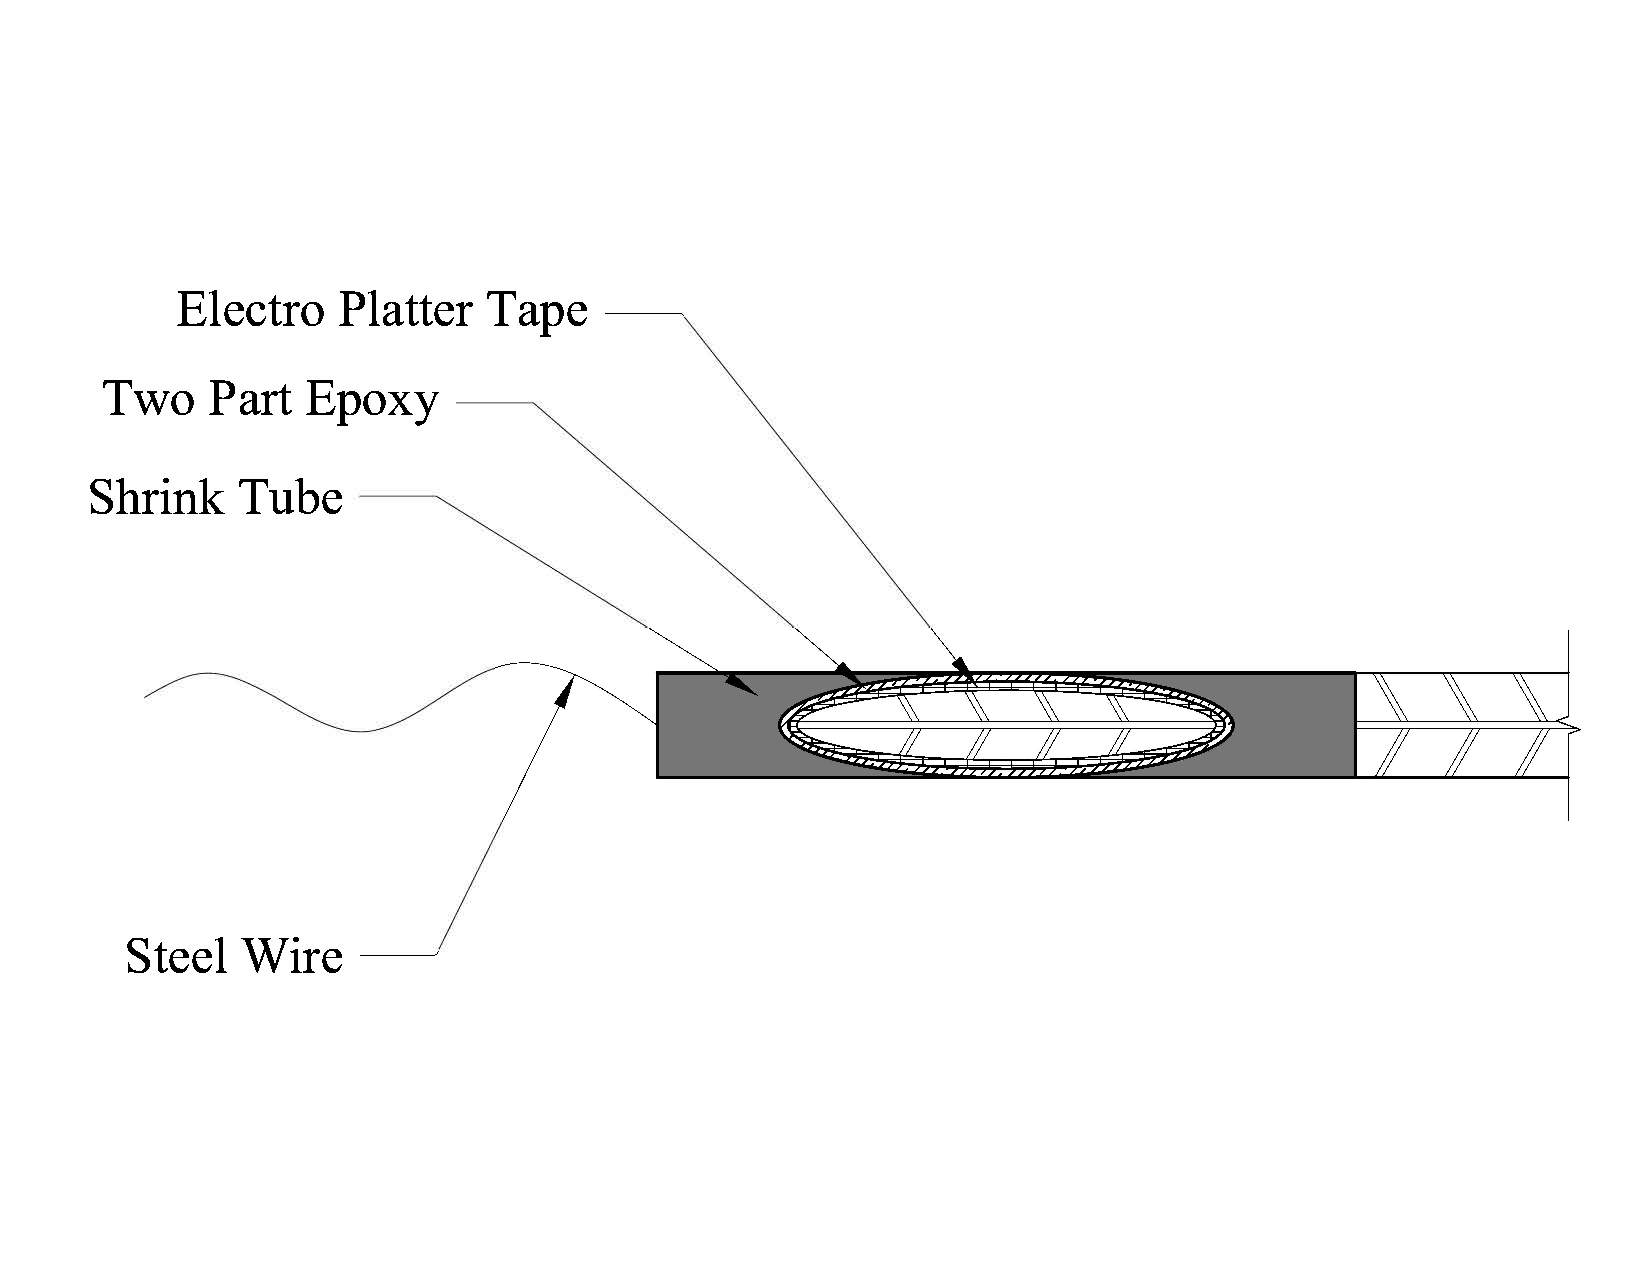
\includegraphics[width=0.9\textwidth]{Chapter-3/figs/Rebar_Ends}
	\caption{Rebars Ends Protection}
	\label{fig:RebarEndsProtection}
\end{figure}


\textbf{Accelerated corrosion  of reinforcing steel}

The accelerated corrosion will be done by using a galvanic cell. Different studies \cite{Ghods2010} have shown that for rebars with pasive films a concentration of 0.3 Moles of sodium chloride ($NaCl$) will start the depassivation process on the rebars. In the study presented here, the specimens will be subjected to a current of 5mA equivalent to $47\mu A/cm^2$. This current is sustained for a period of time according to Faraday's Law until the desired level of corrosion is reached.

\begin{equation}
	t=\frac{\lambda m_{loss} \eta_{specimen} C_{faraday}}{i M_{specimen}}
	\label{eq.FaradayEq}
\end{equation}

\begin{figure}[htbp]
	\centering
	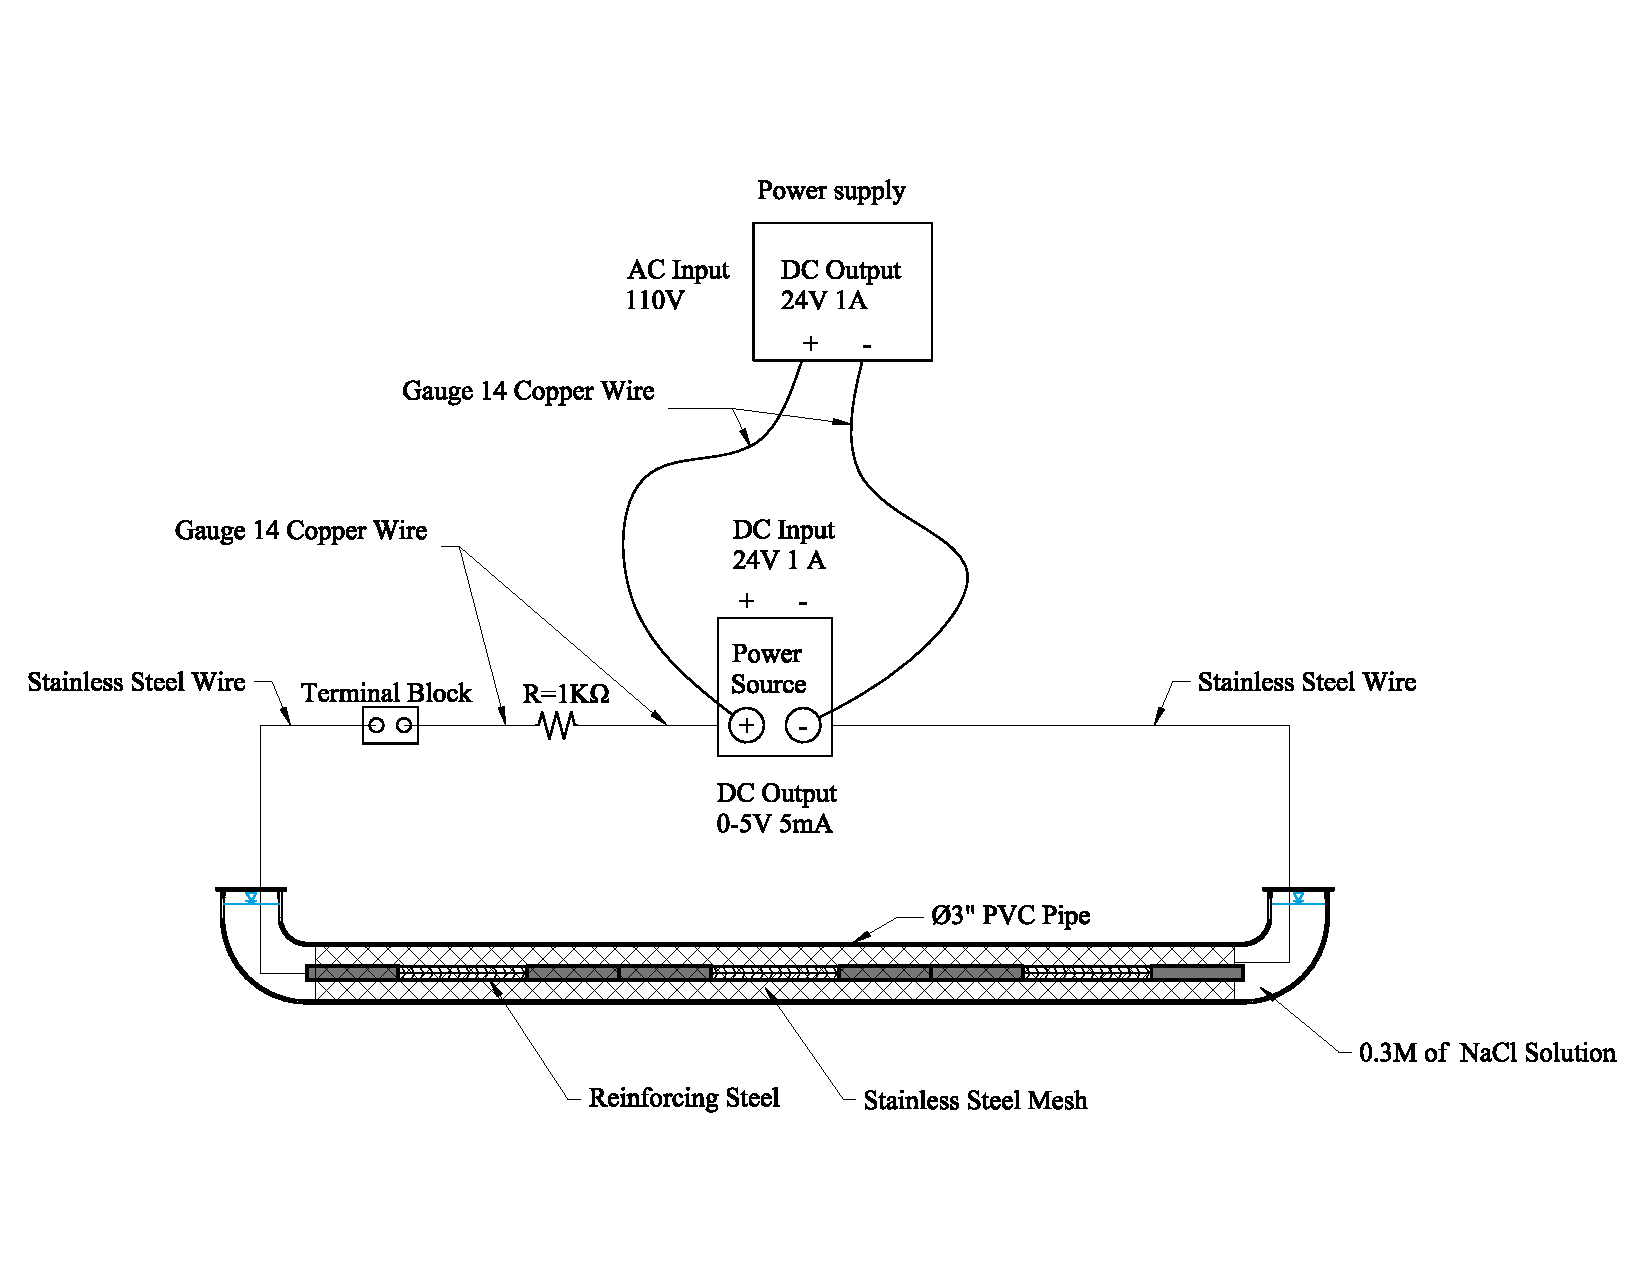
\includegraphics[width=0.9\textwidth]{Chapter-3/figs/AcceleratedCorrosionProcedure}
	\caption{Accelerated corrosion process}
	\label{fig:AcceleratedCorrosion}
\end{figure}

The corrosion levels, the current and the time of application is shown in Table \ref{tab:AcceleratedCorrosionTime}. 

\begin{table}[htbp]
	\caption{Accelerated corrosion times in 3/4" rebar}
	\label{tab:AcceleratedCorrosionTime}
	\centering	
		\begin{tabular}{|l|c|c|}
		\hline
		Corrosion Level (CL) & Mass loss (g)   & time(days)     \\  \hline	
		5\%                  & 1.12            & 9  \\  \hline	
		10\%                 & 2.24            & 18 \\  \hline	
		15\%                 & 3.36            & 27 \\  \hline	
		20\%                 & 4.47            & 36 \\  \hline	
		25\%                 & 5.59            & 45 \\  \hline	
		\end{tabular}
\end{table}
\newpage

\textbf{Tension tests}

A series of tension tests will be performed according to ASTM A370. The main objective of this tests is to evaluate differences in the stress-strain behavior of corroded reinforcing steel. This will determine if there is any reduction in the ductility of steel for this condition.
\newline

\textbf{Buckled bar tension (BBT) test}

One of the limit states that control performance-based design is buckling of reinforcing steel, recent tests have been developed to determine the critical bending strain of buckled reinforcing steel \cite{Barcley2019}. The buckled bar tension (BBT) test simulates bending and tension strain demands on a buckled bar, to determine critical bending strain in buckled rebars. 

Barcley et al \cite{Barcley2019} developed a methodology to calculate local strains on a buckled bar using an LED optical sensor system \cite{NorthernDigitalInc.2020}. The procedure is illustrated in \fref{fig:BBTseq}.

\begin{figure}[htbp]
	\centering
	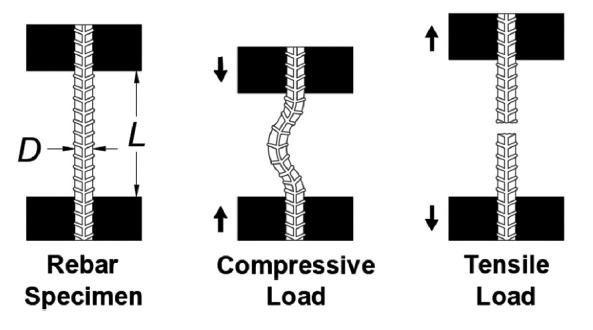
\includegraphics[width=0.7\textwidth]{Chapter-3/figs/BBT_Sequence}
	\caption{BBT Test sequence\cite{Barcley2019}}
	\label{fig:BBTseq}
\end{figure}

The procedure to perform the buckled bar tension test consists of:

\begin{enumerate}
    \item First, place rebar in a univeral testing machine (UTM), and prepare the rebar specimen with LED markers on the surface of the specimen such that the displaced shape of the bar can be measured.
    \item Second, compress the rebar specimen to impose a bending strain of a prescribed level. Barcley et al showed that a fourth order polynomial can be fit to the LED sensors near the buckled region of the bar to obtain the displaced shape ($w$). The bending strain is calculated using solid mechanics principles. Curvature is the second derivative of the displaced shape ($w$) for small displacements is calculated as: 
    \begin{equation}
        \phi=\frac{\frac{d^2w(x)}{dx^2}}{\left[1+\left(\frac{dw(x)}{dx}\right)\right]^\frac{3}{2}}\approx \frac{d^2w(x)}{dx^2}
        \label{eq.CuvatureAprox}
    \end{equation}
    If we assume that the bending is symmetric for the rebar then the strain in the extreme fibers of the rebar is calculated as:
    \begin{equation}
        \varepsilon_{b}=\phi\left(\frac{d_{bl}}{2}\right) 
        \label{eq.BendingStrain}
    \end{equation}    
    Combining equations \eref{eq.CuvatureAprox}, and \eref{eq.BendingStrain} then the bending strain can be expressed as:
    \begin{equation}
        \varepsilon_{b}=\frac{d^2w(x)}{dx^2}\left(\frac{d_{bl}}{2}\right) 
        \label{eq.BendingStrainExpanded}
    \end{equation}
    An example of the calculation of the bending strain is shown in \fref{fig:BBT_Curvature}
    \item Second, Once buckled to the prescribed curvature, the bar is loaded in tension until fracture is observed
    \item Then the process is repeated with a different bar for a different bending strain. After all the tests are performed results from elongation at peak force can be generated as the example shown in \fref{fig:BBT_MaxBendingStrain}. From the results obtained through BBT tests the critical bending strain can be determined. The critical bending strain is defined as the point at which a low elongation under load is obtained. This low elongation results in a brittle fracture of the rebar as shown in \fref{fig:BBT_DuctileBrittle}(b). \fref{fig:BBT_MaxBendingStrain} shows that for bars with rebars the critical bending strain is $\varepsilon_{b}=0.10$ for grade 80 ksi steel.
\end{enumerate}

\begin{figure}[htbp]
    \centering
    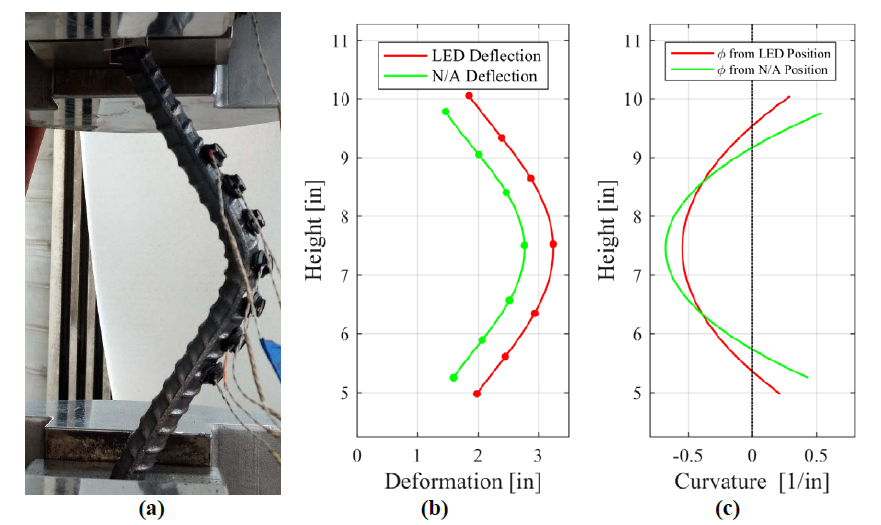
\includegraphics[width=1\textwidth]{Chapter-3/figs/BBT_Curvature}
    \caption{a) Picture of buckled bar; (b) Position of optical markers and adjustment to neutral axis; (c) Calculation of curvature \cite{Barcley2018}}
    \label{fig:BBT_Curvature}
\end{figure}
\begin{figure}
    \centering
    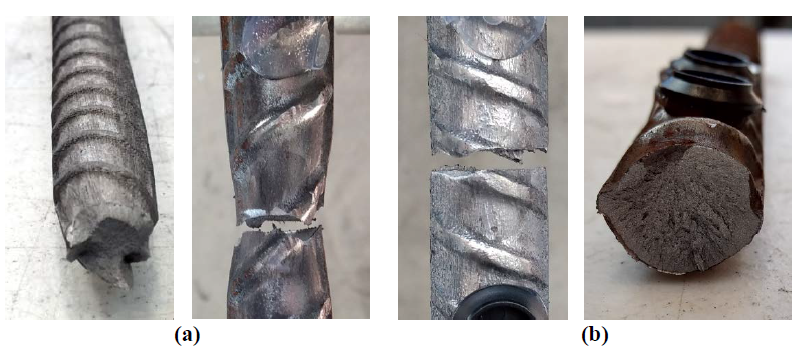
\includegraphics[width=1\textwidth]{Chapter-3/figs/BBT_Ductile_vs_Brittle}
    \caption{(a)Ductile rebar fracture; (b) Brittle rebar fracture \cite{Barcley2018}}
    \label{fig:BBT_DuctileBrittle}
\end{figure}
\begin{figure}[htbp]
    \centering
    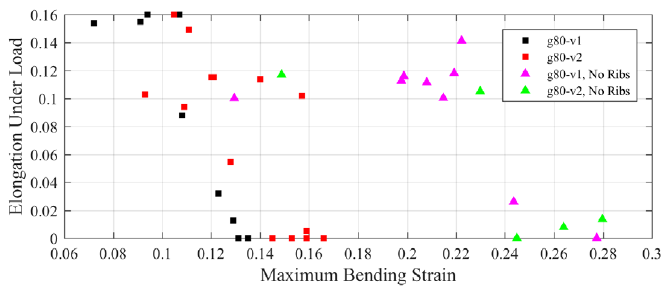
\includegraphics[width=0.8\textwidth]{Chapter-3/figs/BBT_MaxBendignStrain}
    \caption{BBT results for rebars with and without ribs \cite{Barcley2018}}
    \label{fig:BBT_MaxBendingStrain}
\end{figure}

The BBT test is proposed for different levels of corrosion such that any changes on the behavior are studied and incorporated in the analytical model. The proposed test matrix is shown in Table \ref{tab:Test Matrix}. It must be noted that in each corrosion level for the BBT tests, each experiment will correspond to a different prescribes bending strain. The selection for each prescribed bending strains consists in 1) Start with the maximum bending strain determined in previous research to be around $\varepsilon=0.10$ as shown in \fref{fig:BBT_MaxBendingStrain}, 2)if brittle fracture is observed the next test will be at a lower bending strain for example $\varepsilon=0.08$, 3)otherwise higher strains such as $\varepsilon=0.12$ will be evaluated, this is repeated for each corrosion level. It is expected that six tests per corrosion level will be sufficient however, more tests will be performed if necessary. The results obtained will be compared to those of a pristine condition rebar which corresponds to a corrosion level of $CL=0\%$

% Please add the following required packages to your document preamble:
% \usepackage{multirow}
% \usepackage[table,xcdraw]{xcolor}
% If you use beamer only pass "xcolor=table" option, i.e. \documentclass[xcolor=table]{beamer}
\begin{table}[htb]
	\caption{Corroded Rebar Test Matrix}
	\label{tab:Test Matrix}
	\centering	
	\begin{tabular}{|c|c|c|c|}
	\hline
	\multicolumn{4}{|c|}{\cellcolor[HTML]{CC0000}{\color[HTML]{FFFFFF} Corroded rebar test matrix}}                                               \\ \hline
	\multicolumn{1}{|l|}{Test}     & \multicolumn{1}{l|}{Diameter of bar} & \multicolumn{1}{l|}{CL (\%)} & \multicolumn{1}{l|}{Number of Tests} \\ \hline
	                               &                                      & 0                            & 3                                    \\ \cline{3-4} 
	                               &                                      & 5                            & 3                                    \\ \cline{3-4} 
	                               &                                      & 10                           & 3                                    \\ \cline{3-4} 
	                               &                                      & 15                           & 3                                    \\ \cline{3-4} 
	                               &                                      & 20                           & 3                                    \\ \cline{3-4} 
	\multirow{-6}{*}{Tension test} & \multirow{-6}{*}{\#6}                & 25                           & 3                                    \\ \hline
	                               &                                      & 0                            & 6                                    \\ \cline{3-4} 
	                               &                                      & 5                            & 6                                    \\ \cline{3-4} 
	                               &                                      & 10                           & 6                                    \\ \cline{3-4} 
	                               &                                      & 15                           & 6                                    \\ \cline{3-4} 
	                               &                                      & 20                           & 6                                    \\ \cline{3-4} 
	\multirow{-6}{*}{BBT test}     & \multirow{-6}{*}{\#6}                & 25                           & 6                                    \\ \hline
	\end{tabular}
\end{table}

\section{Expected outcomes from experimental phase}

The results from the tension tests will help to establish if the depassivation process in the corroded rebars has an effect on the measured stress-strain relationship of steel as has been observed in previous research which did not considered the depassivation process \cite{Meda2014},\cite{Yuan2017a},\cite{Du2005}. Similarly the results from the BBT tests will show any changes in the critical bending strain of rebars as they corrode. The critical bending train impacts the bar fracture limit state. In the case of corroded rebars it is expected that the critical bending strain will be modified by changes in the mechanical properties of steel due to corrosion, and effects of concentrated corrosion along the surface of the rebars. These two factors we hypothesize will induce fracture at a lower bending strain than those observed in pristine conditions rebars\cite{Barcley2019}.

The results obtained from the experiment will also be used to define the bar fracture limit state for RC columns. Research currently being developed at NC State will provide models that allows to establish bar fracture tensile strain while considering different parameters such as transverse steel spacing, axial load ratio, strength of the concrete to mention a few. The model will be similar to that presented by Barcley et al \cite{Barcley2018} shown in EQ. This model could then be implemented in the analytical model presented in \ref{chap-four}. If fracture occurs at a lower strain in corroded rebars, this implies that the corroded RC columns are prone to reach the fracture bar limit state at a much lower displacement than in a pristine RC column.

Future studies will verify the application of the results found in this research to perform full scale corroded RC column that consider the effect of depassivation in the cyclic behavior of such columns.
\chapter{Methodology}

A methodology that incorporates the different sources of cumulative damage in RC structures is proposed. Different models of aging conditions that modify the material properties are studied, these are then incorporated into the analytical model.

The aging conditions focused on this research are:
\begin{itemize}
	\item Corrosion
	\item Strain aging
\end{itemize}

Other aging conditions will be added later to this study.

\section{Modeling of corrosion for structural analysis}

The previous elements of corrosion explained in the previous sections are incorporated into the structural analysis mainly at the material level. The application can be outlined as follows:
\begin{enumerate}
	\item First the time for initiation of corrosion is calculated with equation \eref{eq.three} 
	\item Then the rate of corrosion is calculated according equation \eref{eq.CorrosionRate}
	\item Following this the diameter of the rebar is reduced and the corrosion level is calculated using equations \eref{eq.CorrosionLevel} \eref{eq.CorrosionEvolution} 
	\item Finally the mechanical properties of the reinforcing steel are modified with the corresponding corrosion level as shown in equation \eref{eq.eleven}
\end{enumerate}

This process is shown in \fref{fig:CorrModel}.

\begin{figure}[htbp]
	\centering
	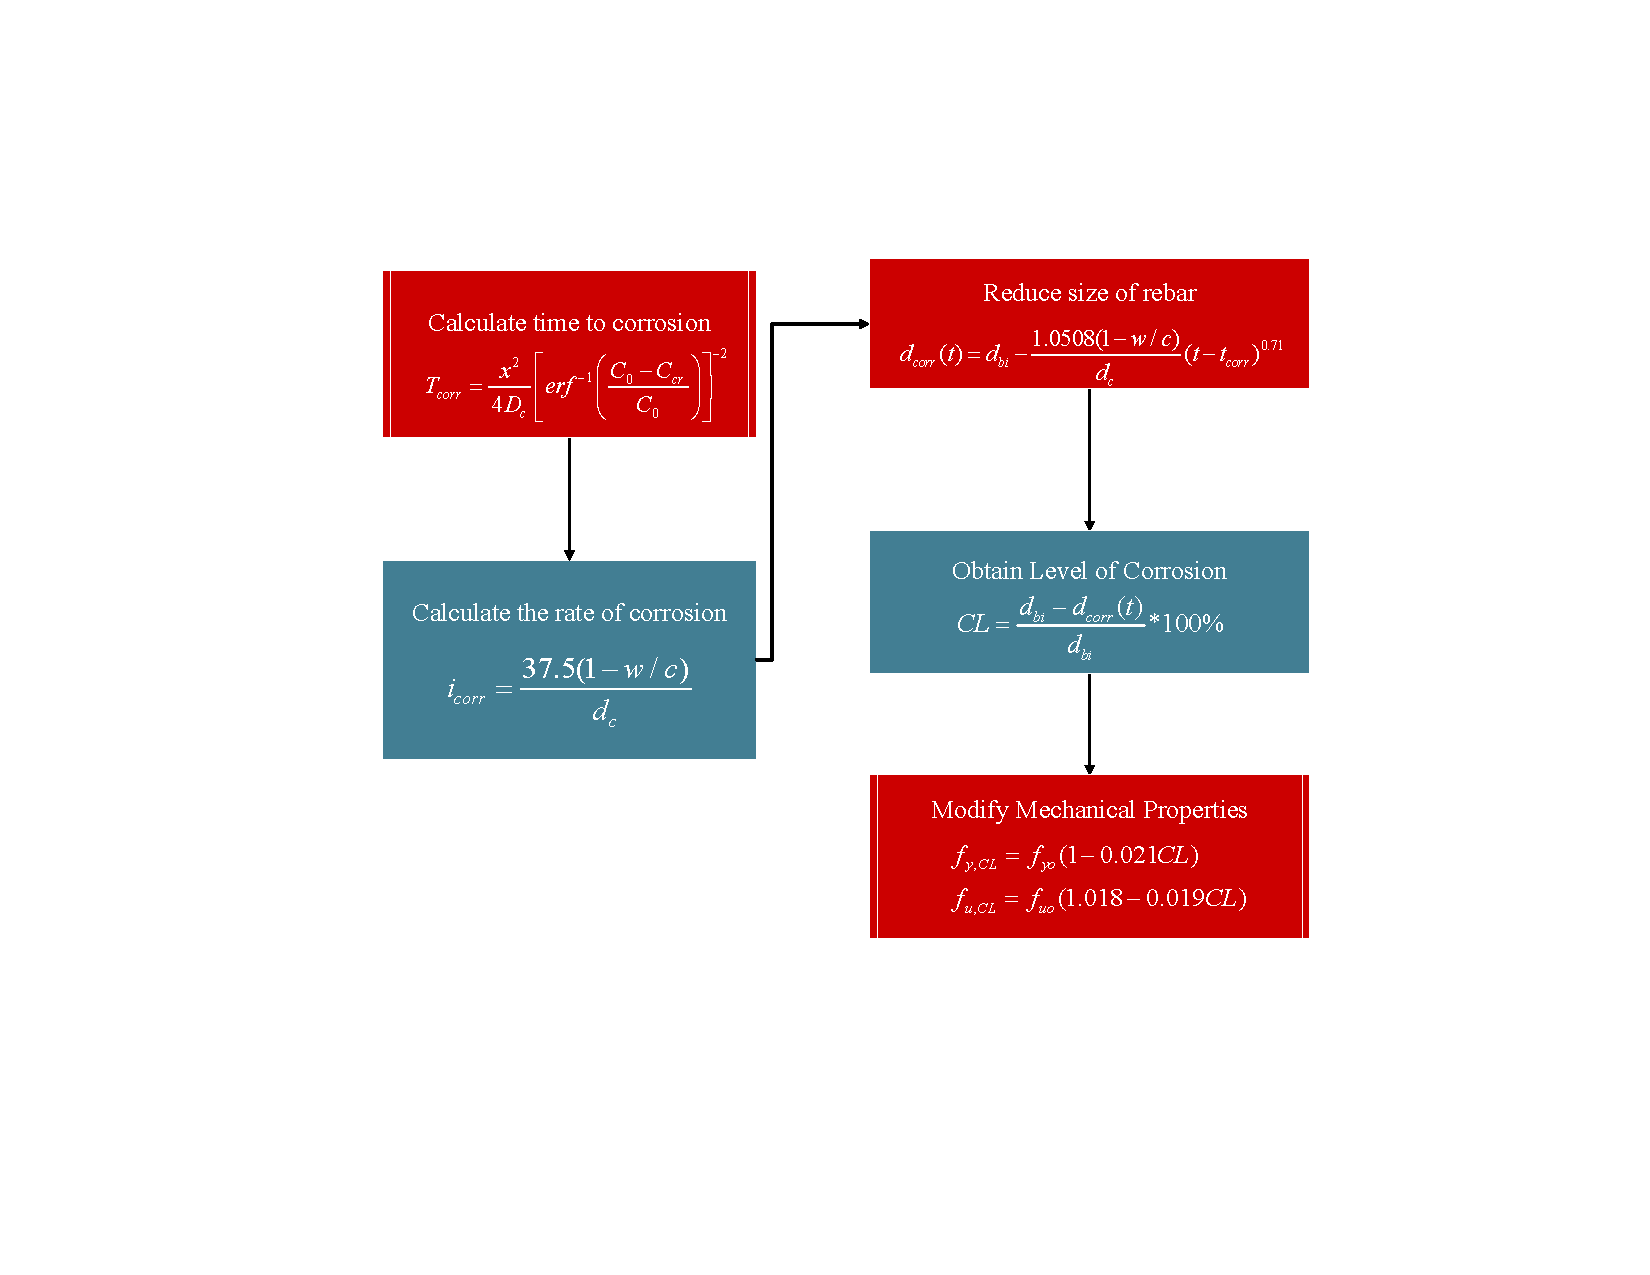
\includegraphics[width=0.7\textwidth]{Chapter-4/figs/Corrosion_Modeling}
	\caption{Corrosion modeling for structural analysis}
	\label{fig:CorrModel}
\end{figure}

This is later incorporated into the nonlinear structural analysis framework using OpenSeesPy \cite{McKenna2010}\cite{Zhu2018}, the framework of this analysis is explained in \textbf{Chapter-4}.


\section{Multiple seismic events}

The evaluation of multiple seismic events is a topic that has been scarcely studied, however their effects have been felt in numerous earthquake sequences such as the Christchurch 2010, Umbria-Marche Earthquake 1997 and the Puerto Rico Earthquakes 2020. The hypothesis is that accumulation of damage will restart in a smaller seismic event to achieve a prescribed limit state, similar to how corrosion and other aging phenomena might impact the intensity needed to achieve a future limit state. 

For this study it has been determined that not all damage in structures are dependent on multiple events but rather their condition when an event occurs as is the case for corrosion. Other damage related phenomenons such as Strain Aging depend on the loading history and are therefore dependent on the history of extreme loading events. It is therefore proposed to study corrosion on a discrete modeling of Main Shocks each independent of the other and to study the effect on Strain Aging by using a sequence of Main Shocks.

\subsection{Earthquake selection}

For this study the NGA2 West Database of earthquake records provided by the Pacific Earthquake and Engineering Research Insitute (PEER) \cite{Ancheta2014} is used. This database consists of 599 different Earthquake events that characterize the ground motions on the west coast of the contiguous United States. The data was filtered according to the following criteria:

\begin{itemize}
	\item Must be an earthquake sequence
	\item Moment Magnitude $M_w \geqslant 5$
	\item $PGA>0.04$
	\item $PGV>1$ cm/s
	\item $Vs_{30}>100m/s$ \& $Vs_{30}<1000$ m/s
	\item Lowest usable frequency is less than 1Hz
	\item $R_{rup}<60km$
\end{itemize}

From this data the main shocks found are the following earthquakes which can be sumarized in \fref{fig:MS_Selection}. Figure \ref{fig:MS_Selection} shows the earthquakes as moment magnitude {Mw} vs rupture distance ($R_{rup}$).

\begin{itemize}
	\item Chi-chi
	\item Managua
	\item Livermore
	\item Northridge
	\item Duzce 
	\item Mammoth lake
\end{itemize}

\begin{figure}[htbp]
	\centering
	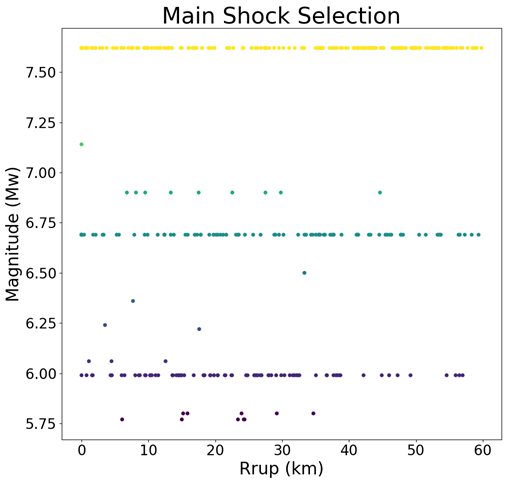
\includegraphics[width=0.6\textwidth]{Chapter-4/figs/MainShock_Selection}
	\caption{Mainshock selection from PEER NGA West2 database}
	\label{fig:MS_Selection}
\end{figure}

\subsection{Discrete Modeling of Main Shock Series}
The discrete modeling of mainshocks consists of using individual earthquakes that occur at different times throughout the life of the structures which correlate to a corrosion level (CL), this can be done for each of the main shocks selected after which the following data is obtained and later analyzed:

\begin{itemize}
	\item Maximum axial strain in confined concrete, cover and reinforcing steel 
Strains
	\item Obtain the probability of exceeding a given limit state $P(\varepsilon >\varepsilon_{LS},IM)$
	\item The earthquakes are characterized according to an intensity measure

\end{itemize}


\subsection{Multiple main shock series}

To simulate the life of a structure a mainshock series consisting of 3 mainshocks for a the life of a structure is considered, three phases are considered:
\begin{enumerate}

	\item At time $t=0$ the structure has pristine conditions
	\item Mainshock 1: pristine conditions are present. No changes to the material properties is present and no accumulation of damage has occurred.
	\item Mainshock 2: significant time after time to corrosion, mainshock 2 occours and  material properties have changed due to corrosion
	\item Mainshock 3: corrosion and strain aging have occurred and further modified the properties of the materials.
\end{enumerate}

%This is shown graphically in \fref{fig:MSSequence}
%
%\begin{figure}[htbp]
%	\centering
%	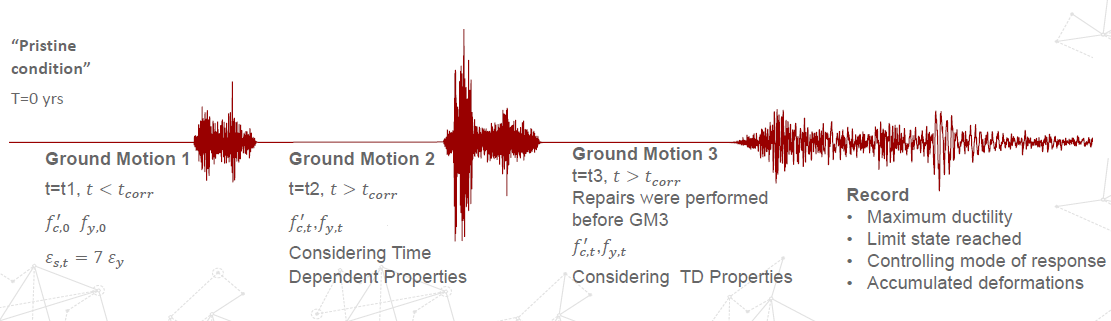
\includegraphics[width=0.9\textwidth]{Chapter-4/figs/MainShock_Sequence}
%	\caption{Mainshock sequence example}
%	\label{fig:MSSequence}
%\end{figure}

Similar to the discrete modeling pf main shock series the following results can be obtained:

\begin{itemize}
	\item Maximum axial strain in confined concrete, cover and reinforcing steel 
Strains
	\item Obtain the probability of exceeding a given limit state $P(\varepsilon\varepsilon_{LS},IM)$
	\item The earthquakes are characterized according to an intensity measure

\end{itemize}

\section{Analytical Model}

\subsection{Cantilever Column}
This study focuses on the behavior of a single degree of freedom (SDOF) system representing a cantilever reinforced concrete column. The column is modeled as shown in \fref{fig:Structural_Model} This structure is modeled in OpenSeesPy \cite{McKenna2010}\cite{Zhu2018} using the $forceBeamColumn$ element \cite{Scott}. The forceBeamColumn element is used with two-point Gauss-Radau integration applied in the hinge regions and two-point Gauss integration applied on the element interior for a total of six integration points \cite{Scott}. The force-based formulation requires only a single element to accurately represent the full nonlinear deformation of the member and the integration scheme selected prevents the loss of objectivity during softening response while also providing integration points at the member ends \cite{Calabrese2010},\cite{Scott}. The element requires the length of plasticity be defined at each end of the member, for which the tension-based rectangular plastic hinge length is calculated using the following expressions \cite{Goodnight2013}:

\begin{equation}
    L_{pc}=k*L_{eff} + 0.4D
    \label{eq:LP_Comp}
\end{equation}
\begin{equation}
	k=0.2*(Fu/Fy - 1) \leqslant 0.08
	\label{eq:K_Lp}
\end{equation}
\begin{equation}
    L_{pt}=L_{pc}+\gamma*D
    \label{eq:LP_Tension}
\end{equation}

For single bending the parameter $\gamma$ is:
\begin{equation}
    \gamma=0.33
    \label{eq:Gamma_LPt}
\end{equation}

The two-point Gauss-Radau integration is applied such that each end node integration is weighted equal to the specified plastic hinge length, as illustrated in \fref{fig:Fiber_PlasticHinge}. Therefore, strains recorded at the end sections represent accurate values even in the case where deformation localizes to the ends from strain-softening behavior. For the case of the cantilever column considered, only one plastic hinge length is defined, and the opposite end is given an arbitrary unit length. 

\begin{figure}[htbp]
	\centering
	\includegraphics[width=0.75\textwidth]{Chapter-4/figs/StructuralModel_01}
	\caption{Structural Model a) SDOF Column b) Structural Model}
	\label{fig:Structural_Model}
\end{figure}

\begin{figure}[htbp]
	\centering
	\includegraphics[width=0.9\textwidth]{Chapter-4/figs/fbc_PlasticHinge}
	\caption{End point plastic hinge method \cite{Scott}}
	\label{fig:Fiber_PlasticHinge}
\end{figure}

The section of the column is shown in \fref{fig:ColumnSection}, the section is discretized with concrete and steel material fibers. Concrete fibers are modeled using the $Concrete01$ material, modified for confined material strength based on the Mander confined concrete model \cite{Mander1988}. The $Steel02$ material, based on the Giuffre-Menegotto-Pinto model \cite{Filippou1983} is used for the longitudinal reinforcement with recommended parameters ($b = 0.01, R0 = 20, cR1 = 0.925, cR2 = 0.15$). 

\begin{figure}[htbp]
	\centering
	\includegraphics[width=0.7\textwidth]{Chapter-4/figs/StructuralModel_Section}
	\caption{Section of the RC Column}
	\label{fig:ColumnSection}
\end{figure}
\subsection{Strain Penetration}

The strain penetration considers the additional deformation due to anchorage of the reinforcement into the foundation, since the strains of tension in the reinforcement will drop to zero at a depth equal to the true development length of the rebar \cite{Priestley2007}. Experimental studies have generally reported that this end rotation contributes up to 35\% to the lateral deformation of flexural members\cite{Zhao2007} and it is, therefore, important to incorporate into the analytical model. A way to capture this effect is by using a zero-length section element implemented in the nonlinear fiber-based analysis of concrete structures, this is available in the material library of OpenSeesPy as $Bond SP1$ \cite{Zhao2007} this is the material model used for the steel fibers of the zero-length section element.

The required parameters for this model are:
\begin{itemize}
	\item $F_{y}$ Yield strength of the reinforcement steel
	\item $S_{y}$ Rebar slip at member interface under yield stress (see \eref{eq.Rebar_Slip})
	\item $F_{u}$ Ultimate strength of the reinforcement steel
	\item $S_{u}$ Rebar slip at the loaded end at the bar fracture strength a value of $35 S_{y}$ is recommended \cite{Zhao2007}
	\item $b$ Initial hardening ratio in the monotonic slip vs. bar stress response $b=0.45$ is recommended \cite{Zhao2007}
	\item $R$ Pinching factor for the cyclic slip vs. bar response $R=1.01$ is recommended \cite{Zhao2007}
	\item $d_b$ Rebar diameter
	\item $f'c$ Concrete compressive strength of the adjoining connection member
	\item $\alpha$ Parameter used in the local bond-slip relation and can be taken as $\alpha=0.4$ in accordance with CEB-FIP Model Code 90 \cite{CEB1993}
\end{itemize}

Bar slip is calculated as:
\begin{equation}
	S_{y}(in)=0.1\left(\frac{d_{b}F_{y}}{4000\sqrt{f'_{c}}}\left(2\alpha+1\right)\right)^{\frac{1}{\alpha}}+0.013 (in)
	\label{eq.Rebar_Slip}
\end{equation}
\subsection{Design Limit States}
Design limit states are defined based on strains in the material since they can more accurately represent the different performance levels of a structure. Structure limit states are defined for tension strains in the rebars or compression strains in the concrete core. The values recommended in typical performance-based design of reinforced concrete bridge columns are shown in Table  \ref{tab:DesignLimitStates}. The serviceability limit states correspond to the compression strain at which concrete cover begins to crush and the peak tension strain which results in residual crack widths of approximately 1 mm. These limits are generally accepted as nominal limit states for RC members. The compression limit state for damage control is defined by the expression shown in eq. \ref{eq:ec_DamageControl} and it refers to the compression strain in the confined concrete at which fracture of the transverse reinforcement confining the core occurs \cite{Priestley2007}. This equation is obtained using the strain-energy balance between that absorbed by the confined core concrete and the capacity of the confining steel. The tension damage control limit state is defined by the strain at the onset of buckling which can be expressed according to \ref{eq:es_DamageControl}, this equation demonstrated accurate predictions of the onset of bar buckling on physical tests in SDOF Concrete Column \cite{Goodnight2016}. The bar buckling limit state could change as a result of the experimental campaign proposed in Chapter 4.

\begin{equation}
    \varepsilon_{c,spiral yield}=0.009-0.3\frac{A_{st}}{A_{g}} +3.9\frac{f_{yhe}}{E_{s}}
    \label{eq:ec_DamageControl}
\end{equation}

\begin{equation}
    \varepsilon_{s,BB}=0.03+700\rho_{s}  \frac{f_{yhe}}{E_{s}} -0.1\frac{P}{f'_{c}A_{g}}
    \label{eq:es_DamageControl}
\end{equation}


\begin{table}[htbp]
	\caption{Design Limit States}
	\label{tab:DesignLimitStates}
	\centering	
		\begin{tabular}{|l|c|c|}
		\hline
		\cellcolor[HTML]{CC0000}{\color[HTML]{FFFFFF}Limit State} & \cellcolor[HTML]{CC0000}{\color[HTML]{FFFFFF}Concrete Limit State $\varepsilon_{c} (in/in)$} & \cellcolor[HTML]{CC0000}{\color[HTML]{FFFFFF}Reinforcing Steel Limit State $\varepsilon_{s} (in/in)$}\\  \hline	
		Serviciability       & 0.004                           & 0.015  \\  \hline	
		Damage Control       & Eq. \ref{eq:ec_DamageControl}   & Eq. \ref{eq:es_DamageControl}\\  \hline
		\end{tabular}
\end{table}
 
\section{Comparison with existing physical Tests}
\subsection{Pristine Condition Columns}

Goodnight et al performed a total of 30 circular RC columns quasi-static tests to evaluate strain limit states \cite{Goodnight2016}. From this set of tests, a sample of one was taken to calibrate the analytical model. The test performed by Goodnight et al on an SDOF cantilever column shows similar geometry to that presented in \fref{fig:Fiber_PlasticHinge}. The parameters used in this large scale test were:

\begin{itemize}
	\item Diameter $D = 24.0 inch$
	\item Height of the column $L = 8.0 ft$
	\item Yield strength of steel $f_{y} = 574.0 MPa$
	\item Ultimate strength of steel $f_{u} = 753.3 * MPa$
	\item Longitudinal steel volumetric ratio $\rho_{s} = 1.5\% $
	\item Transverse steel volumetric ratio $\rho_{v} = 1.0\% $
	\item Strength of concrete at 8 days $f'_{c} = 39.8 MPa$
\end{itemize}

The analytical model utilized these parameters to compare the results from the model to the experimental results. The results from the analysis show good agreement with the experimental results as evidenced in \fref{fig:ModelCalibration}. This assures that the results obtained from the model predict the overall system behavior and can be used to analyze other configurations of the structural model.

\begin{figure}[htbp]
	\centering
	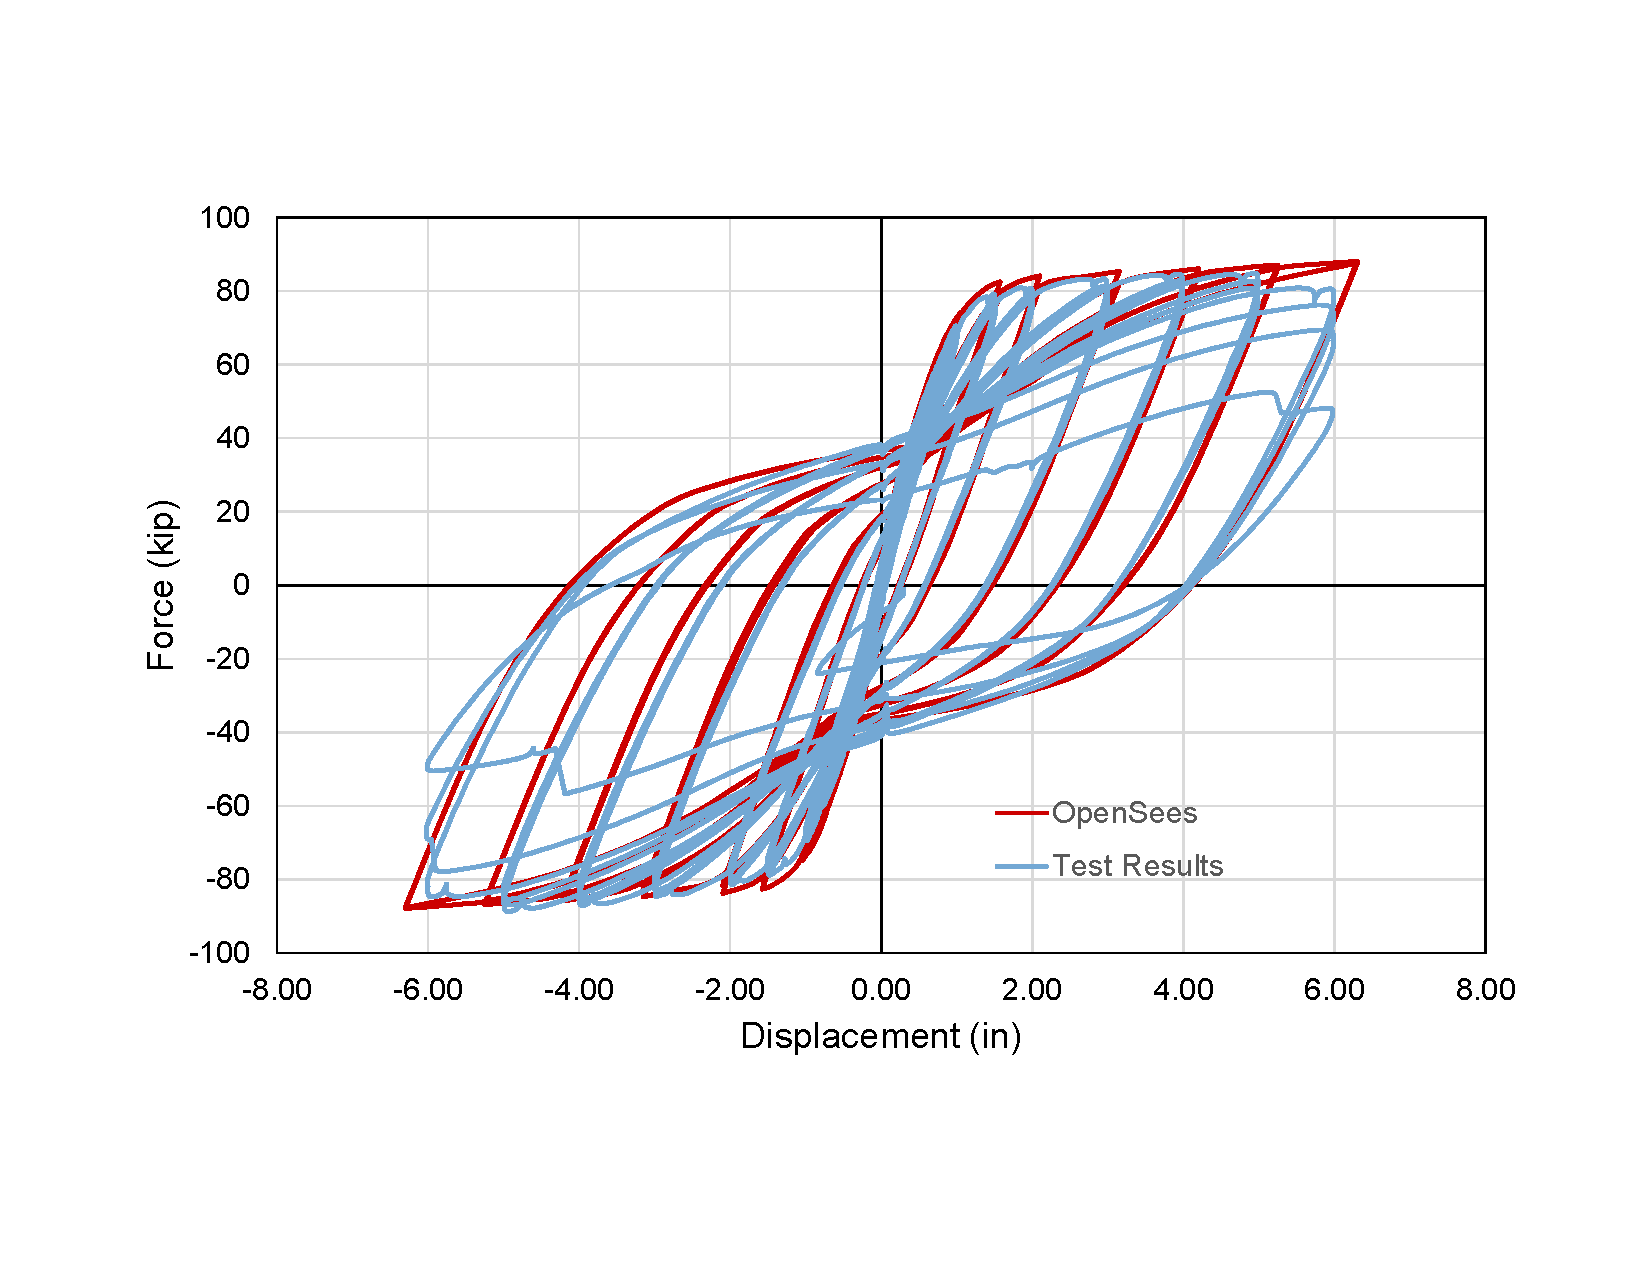
\includegraphics[width=0.7\textwidth]{Chapter-4/figs/Model_Calibration_Goodnight2016}
	\caption{Force-Displacement results from experimental results \cite{Goodnight2013} and analytical model}
	\label{fig:ModelCalibration}
\end{figure}
\subsection{Accelerated Corrosion Columns}
Similarly, Ma et al performed a series of quasi-static tests on RC columns with different corrosion levels and axial load ratios \cite{Ma2012}. From their study, the test with a corrosion level $CL=9.5\%$ was taken for calibration since the other tests presented in their study had excessively high axial load ratios which are not common in RC bridges. The results from Ma et al test	\cite{Ma2012} were used to compare against the analytical model. The column had the following parameters:
\begin{itemize}
	\item Diameter $D = 260.0 mm$
	\item Height of the column $L = 820.0 mm$
	\item Yield strength of steel $f_{y} = 375.0$ MPa
	\item Ultimate strength of steel $f_{u} = 572.3$ MPa
	\item Longitudinal steel volumetric ratio $\rho_{s} = 1.5\% $
	\item Transverse steel volumetric ratio $\rho_{v} = 1.0\% $
	\item Strength of concrete at 8 days $f'_{c} = 39.8$ MPa
	\item Corrosion level $CL=9.5\%$
\end{itemize}

In the analysis equation \eref{eq.eleven} is used to modify the material properties of the reinforcing steel, to consider the effects of corrosion. Figure \ref{fig:ModelCalibration_Corrosion} shows that the results obtained from the analytical model capture the response of the structure with some accuracy. Ma et al \cite{Ma2012} did not report if bar buckling and bar fracture occurred during the test. However, the hysteresis curve shown in their study suggests that some damage limit state was reached. To corroborate this, equation \eref{eq:es_DamageControl} is used to determine the bar buckling limit state ($\varepsilon_{s,BB}=0.024$), this is then compared to the analytical model results shown in figure \fref{fig:ModelCalibration_Corrosion_Hysteresis}. The results show a peak tension strain of $\varepsilon_{s}=0.023$. This result is close to the value obtained using equation \eref{eq:es_DamageControl}, thus pointing out the likelihood that the bar buckling limit state was observed during this test. While these results are close, it is still not clear if equation \eref{eq:es_DamageControl} captures the behavior of the buckling limit state for corroded rebars, therefore, the proposed corroded BBT test will show if corrosion affects the behavior of buckled bars.

\begin{figure}[htbp]
	\centering
	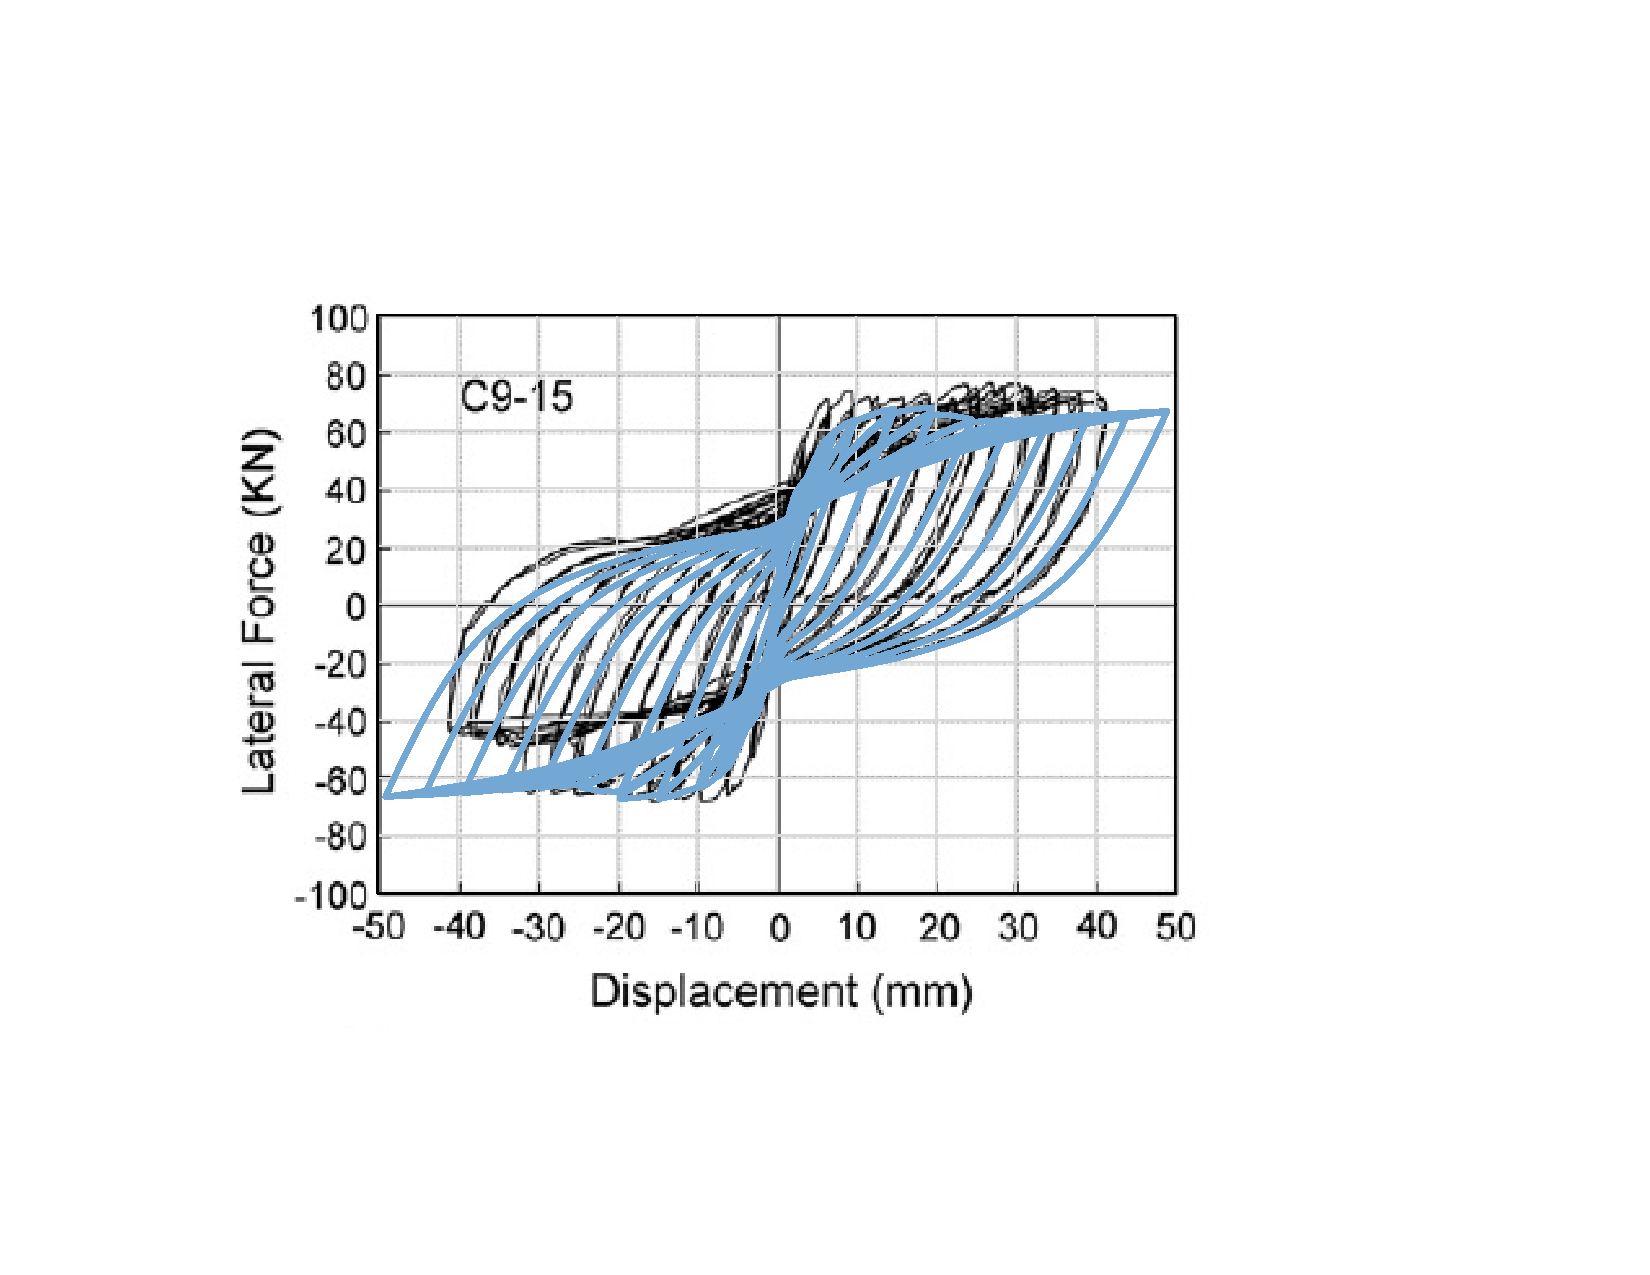
\includegraphics[width=0.7\textwidth]{Chapter-4/figs/Model_Calibration_Ma2012}
	\caption{Force-Displacement results from experimental RC column with corrosion in logitudinal bar (CL=9.5\%) results \cite{Ma2012} and analytical model (shown in lightblue)}
	\label{fig:ModelCalibration_Corrosion}
\end{figure}
\begin{figure}[htbp]
	\centering
	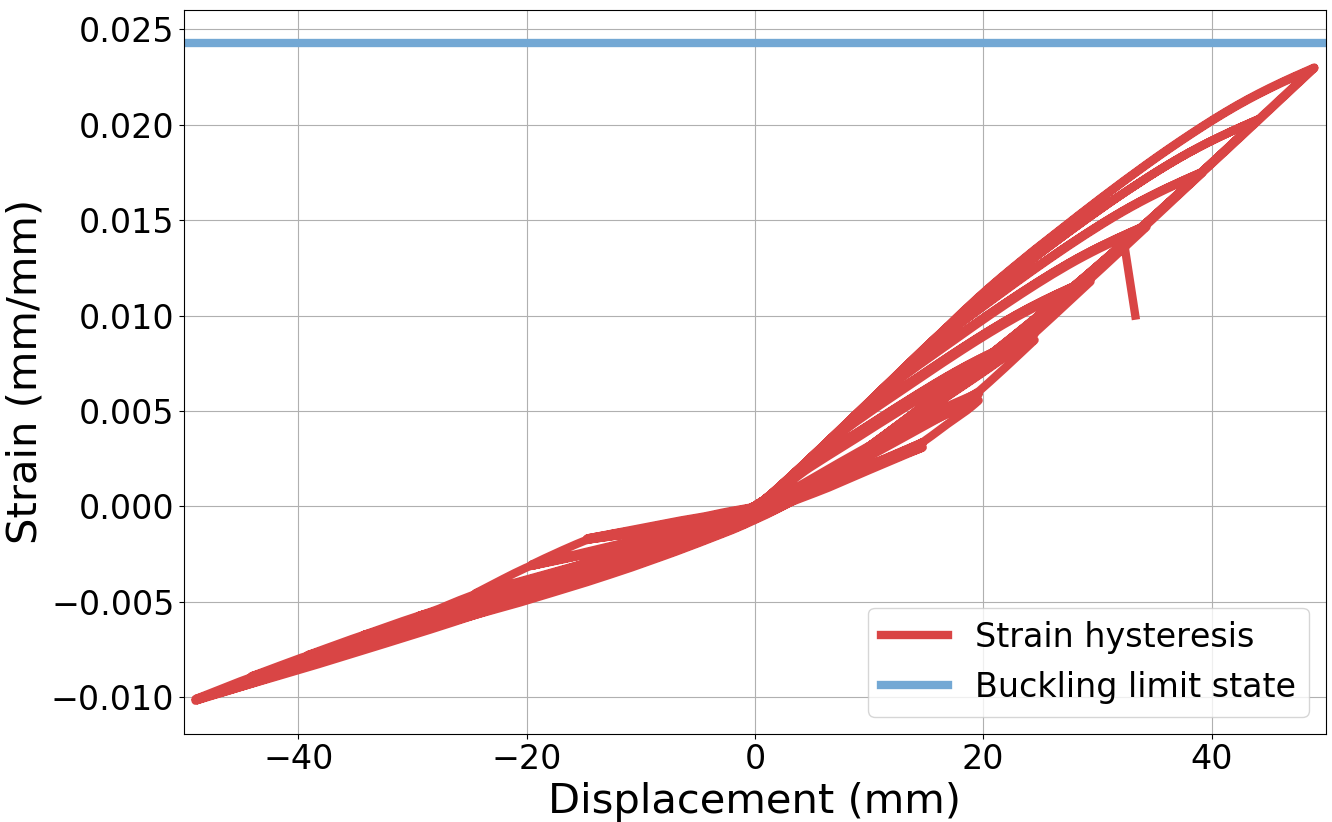
\includegraphics[width=0.9\textwidth]{Chapter-4/figs/MaEtAl_StrainHisteresis}
	\caption{Strain hysteresis from experimental RC column with corrosion in logitudinal bar (CL=9.5\%) results from analytical model}
	\label{fig:ModelCalibration_Corrosion_Hysteresis}
\end{figure}
\newpage

\section{Analytical Framework}

An analytical framework is established to obtain the change in the structure performance due to aging conditions and evaluate the effect of multiple seismic events. Therefore, a series of nonlinear time history analyses (NLTHA) will be performed. From these analyses, it is possible to determine the effects of damage in the performance of structures. The proposed analytical framework process consists of:

\begin{enumerate}
	\item Geometrical Properties of the SDOF column 
	\item Properties of the material are evaluated (i.e. water to cement ratio, cover)
	\item For equal periods of time the time dependent properties are modified
	\item Nonlinear time history analyses are performed for discrete ground motions or sequence of ground motions
	\item Results are obtained and evaluated
\end{enumerate}

The analysis matrix for the corrosion aging phenomenon that will be analyzed in this study is shown in Table \ref{tab:AnalysisMatrix}. The area or extent covered in the analysis corresponds to the range of variables that are common for RC columns in bridges.

\begin{table}[htb]
	\caption{Analysis Matrix}
	\label{tab:AnalysisMatrix}
	\centering
\begin{tabular}{{|l|c|c|}}
\multicolumn{3}{c}{\cellcolor[HTML]{C90000}{\color[HTML]{FFFFFF} ANALYSIS MATRIX}} \\	\hline
Description                            & Parameter        & Range                  \\	\hline
Diameter of Column                     & D                & 30-90 in               \\	\hline
Column Length to Diameter Ratio        & L/D              & 2-8                    \\	\hline
Longitudinal Ratio                     & $\rho_s$         & 0.01-0.04              \\	\hline
Transverse Volumetric Ratio            & $\rho_v$         & 0.005-0.015            \\	\hline
Axial Load Ratio                       & ALR              & 0.05-0.2               \\	\hline
water to cement ratio                  & w/c              & 0.36-0.6               \\	\hline
cover                                  & c                & 1.5-3 in               \\	\hline
Time/Condition                         & CL               & 5\%-20\%               \\	\hline
\end{tabular}
\end{table}

%This procedure has been summarized in the form of a flow chart presented in \fref{fig:NLTHA_Framework}
%
%\begin{figure}[htbp]
%	\centering
%	\includegraphics[width=0.9\textwidth]{Chapter-4/figs/AnalysisFramework_01}
%	\caption{Analysis Framework Flowchart}
%	\label{fig:NLTHA_Framework}
%\end{figure}
%
%\section{Earthquake selection}
%\lipsum[4]
\section{Results from NLTHA}
This section presents the results obtained from a non-linear time history analysis (NLTHA) performed using OpenSeesPy \cite{Zhu2018}. The structure was subjected to a total of 18 earthquake records. The main responses obtained from these analyses correspond to the maximum strain obtained for the different levels of corrosion. 

The structure used for this results currently corresponds to the parameters shown in section 5.2.1. The structure was analyzed for a range of corrosion levels [1.5\%-13\%] in the longitudinal rebars.

\subsection{Effect on structure response}
An example of the results obtained using NLTHA, figures \fref{fig:Force-Displacement_Results} and \fref{fig:Steel_Stress_Strain_Response} are presented. These results are extracted from the response of the structure to the Chi-Chi earthquake. \fref{fig:Force-Displacement_Results} shows the global system response and \fref{fig:Steel_Stress_Strain_Response} shows the stress-strain response of the extreme fiber of reinforcing steel. These results show that as corrosion increases the demands imposed on the structure increases too. Therefore an increase in the probability of reaching a limit state increases as corrosion increases.

\begin{figure}[htbp]
	\centering
	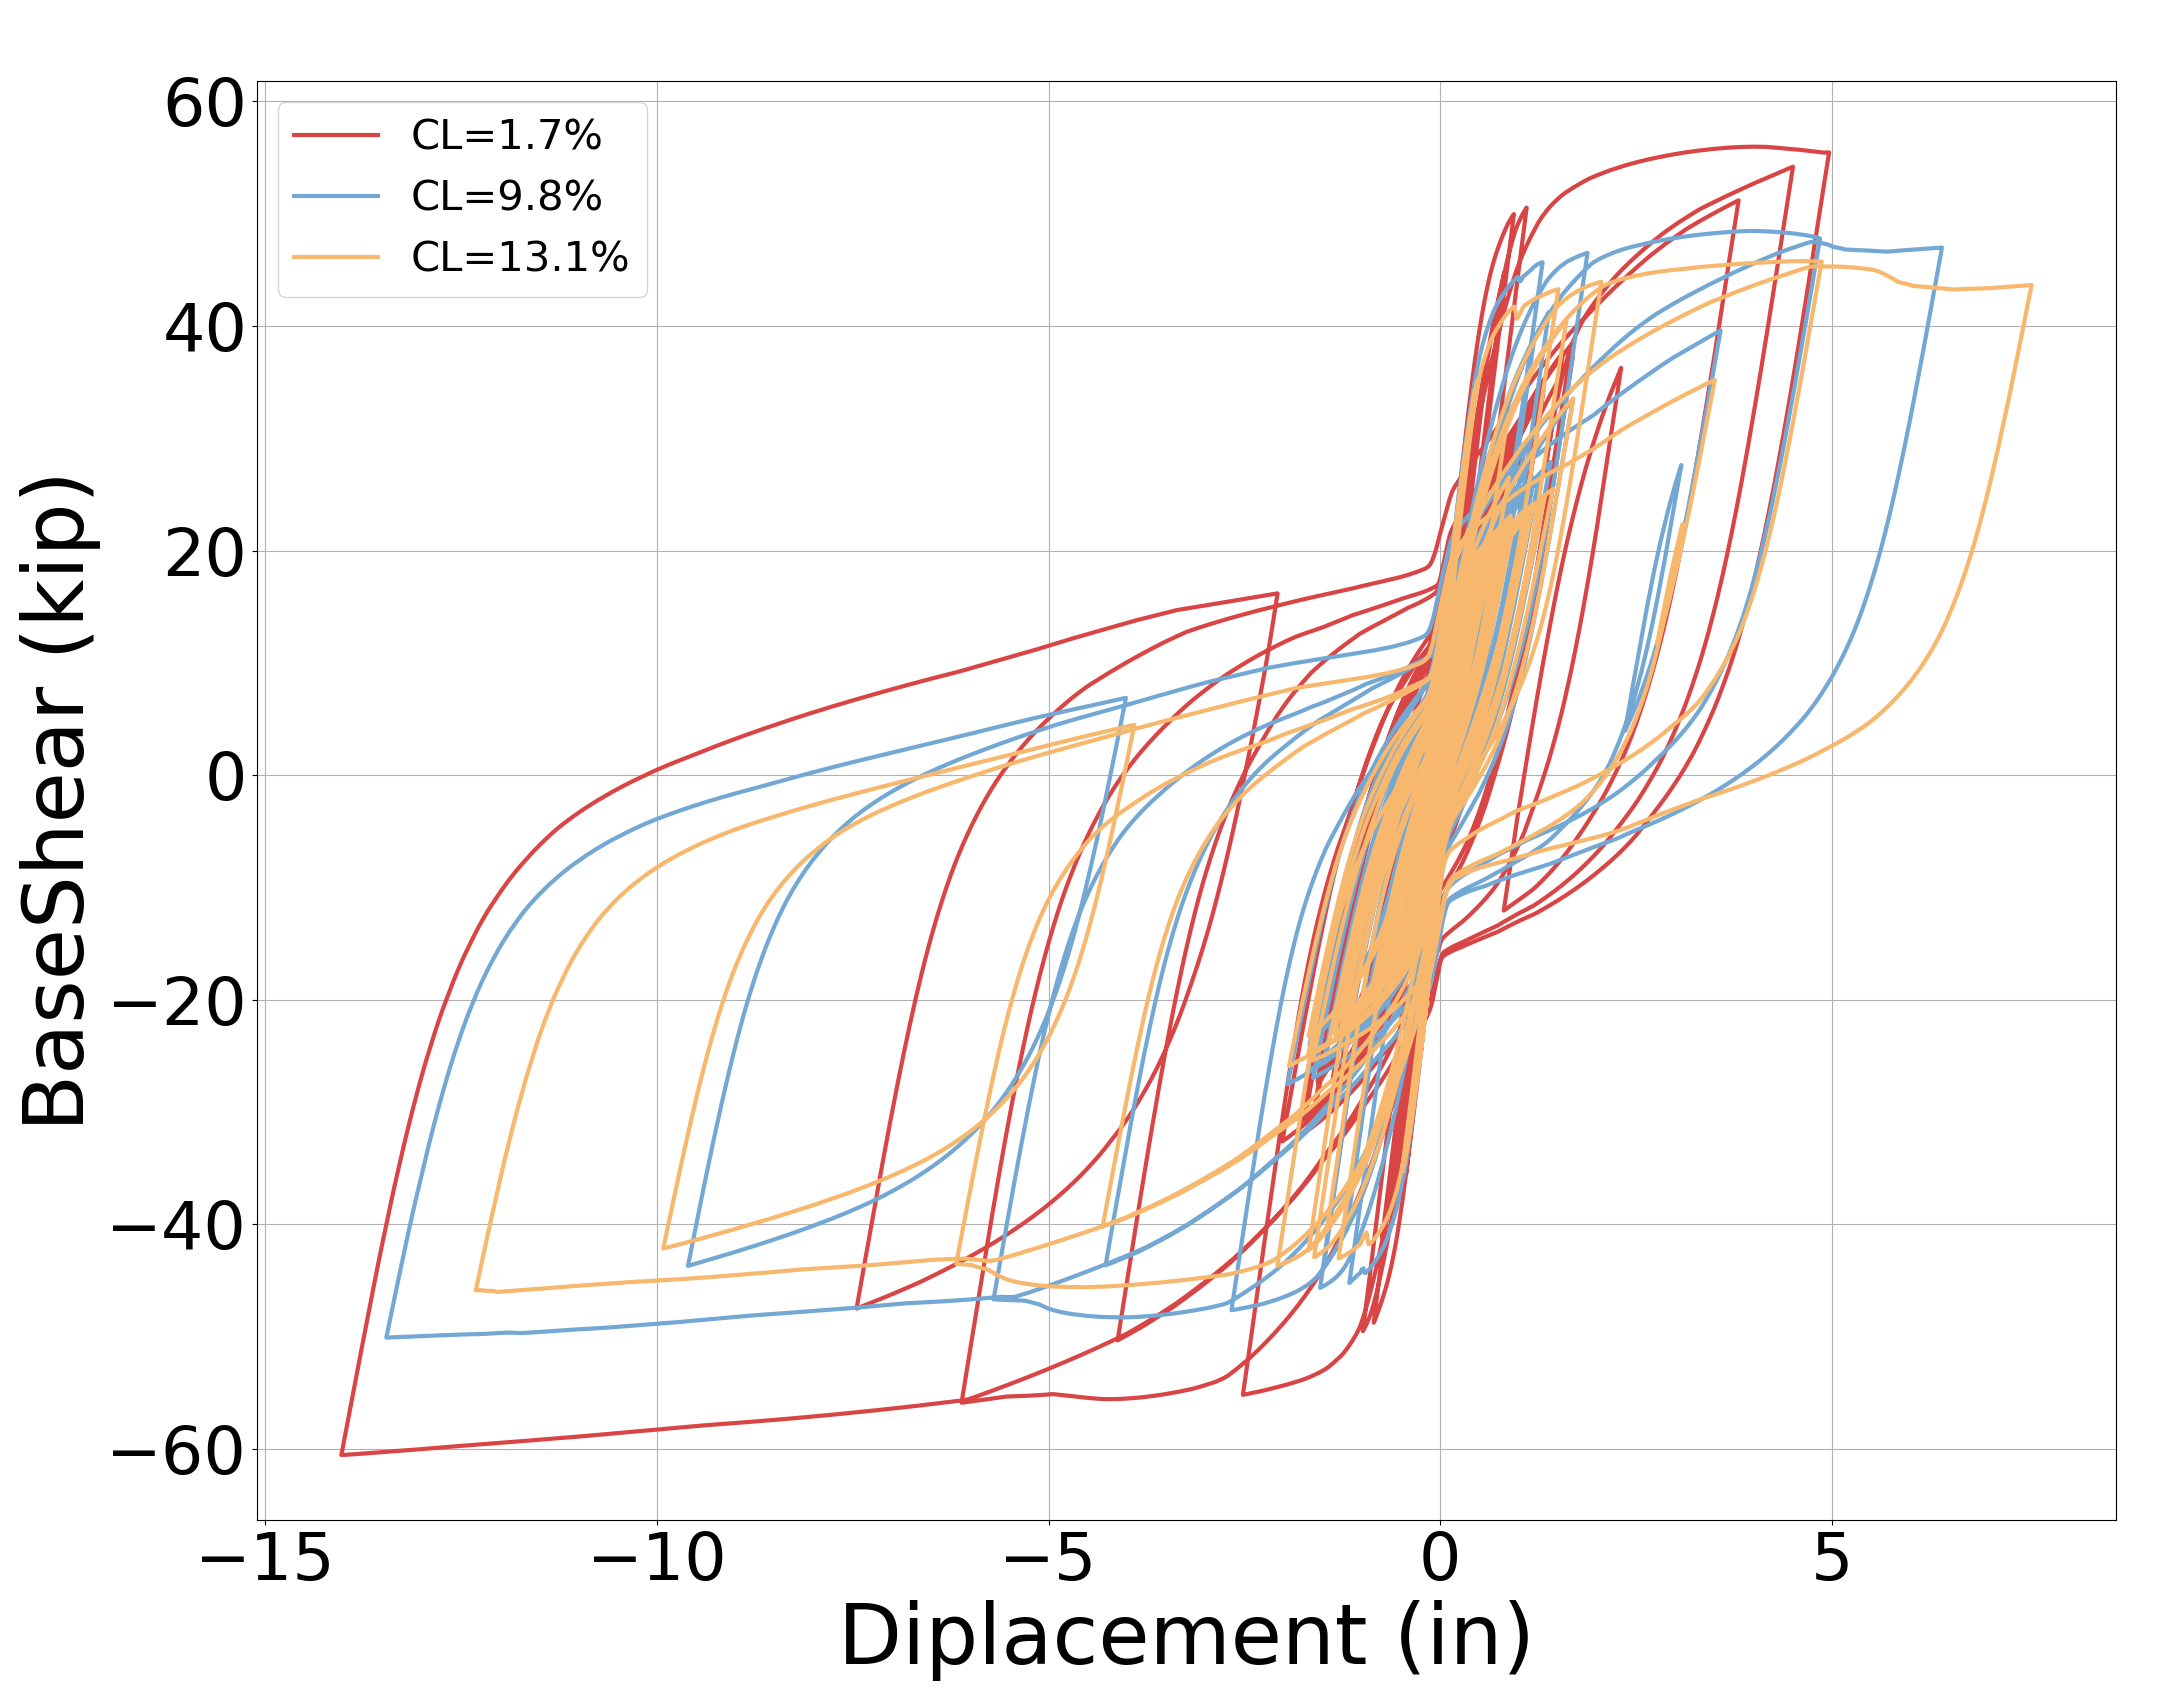
\includegraphics[width=0.65\textwidth]{Chapter-4/figs/ForceDisplacement_01}
	\caption{Force-Displacement results}
	\label{fig:Force-Displacement_Results}
\end{figure}
\begin{figure}[htbp]
	\centering
	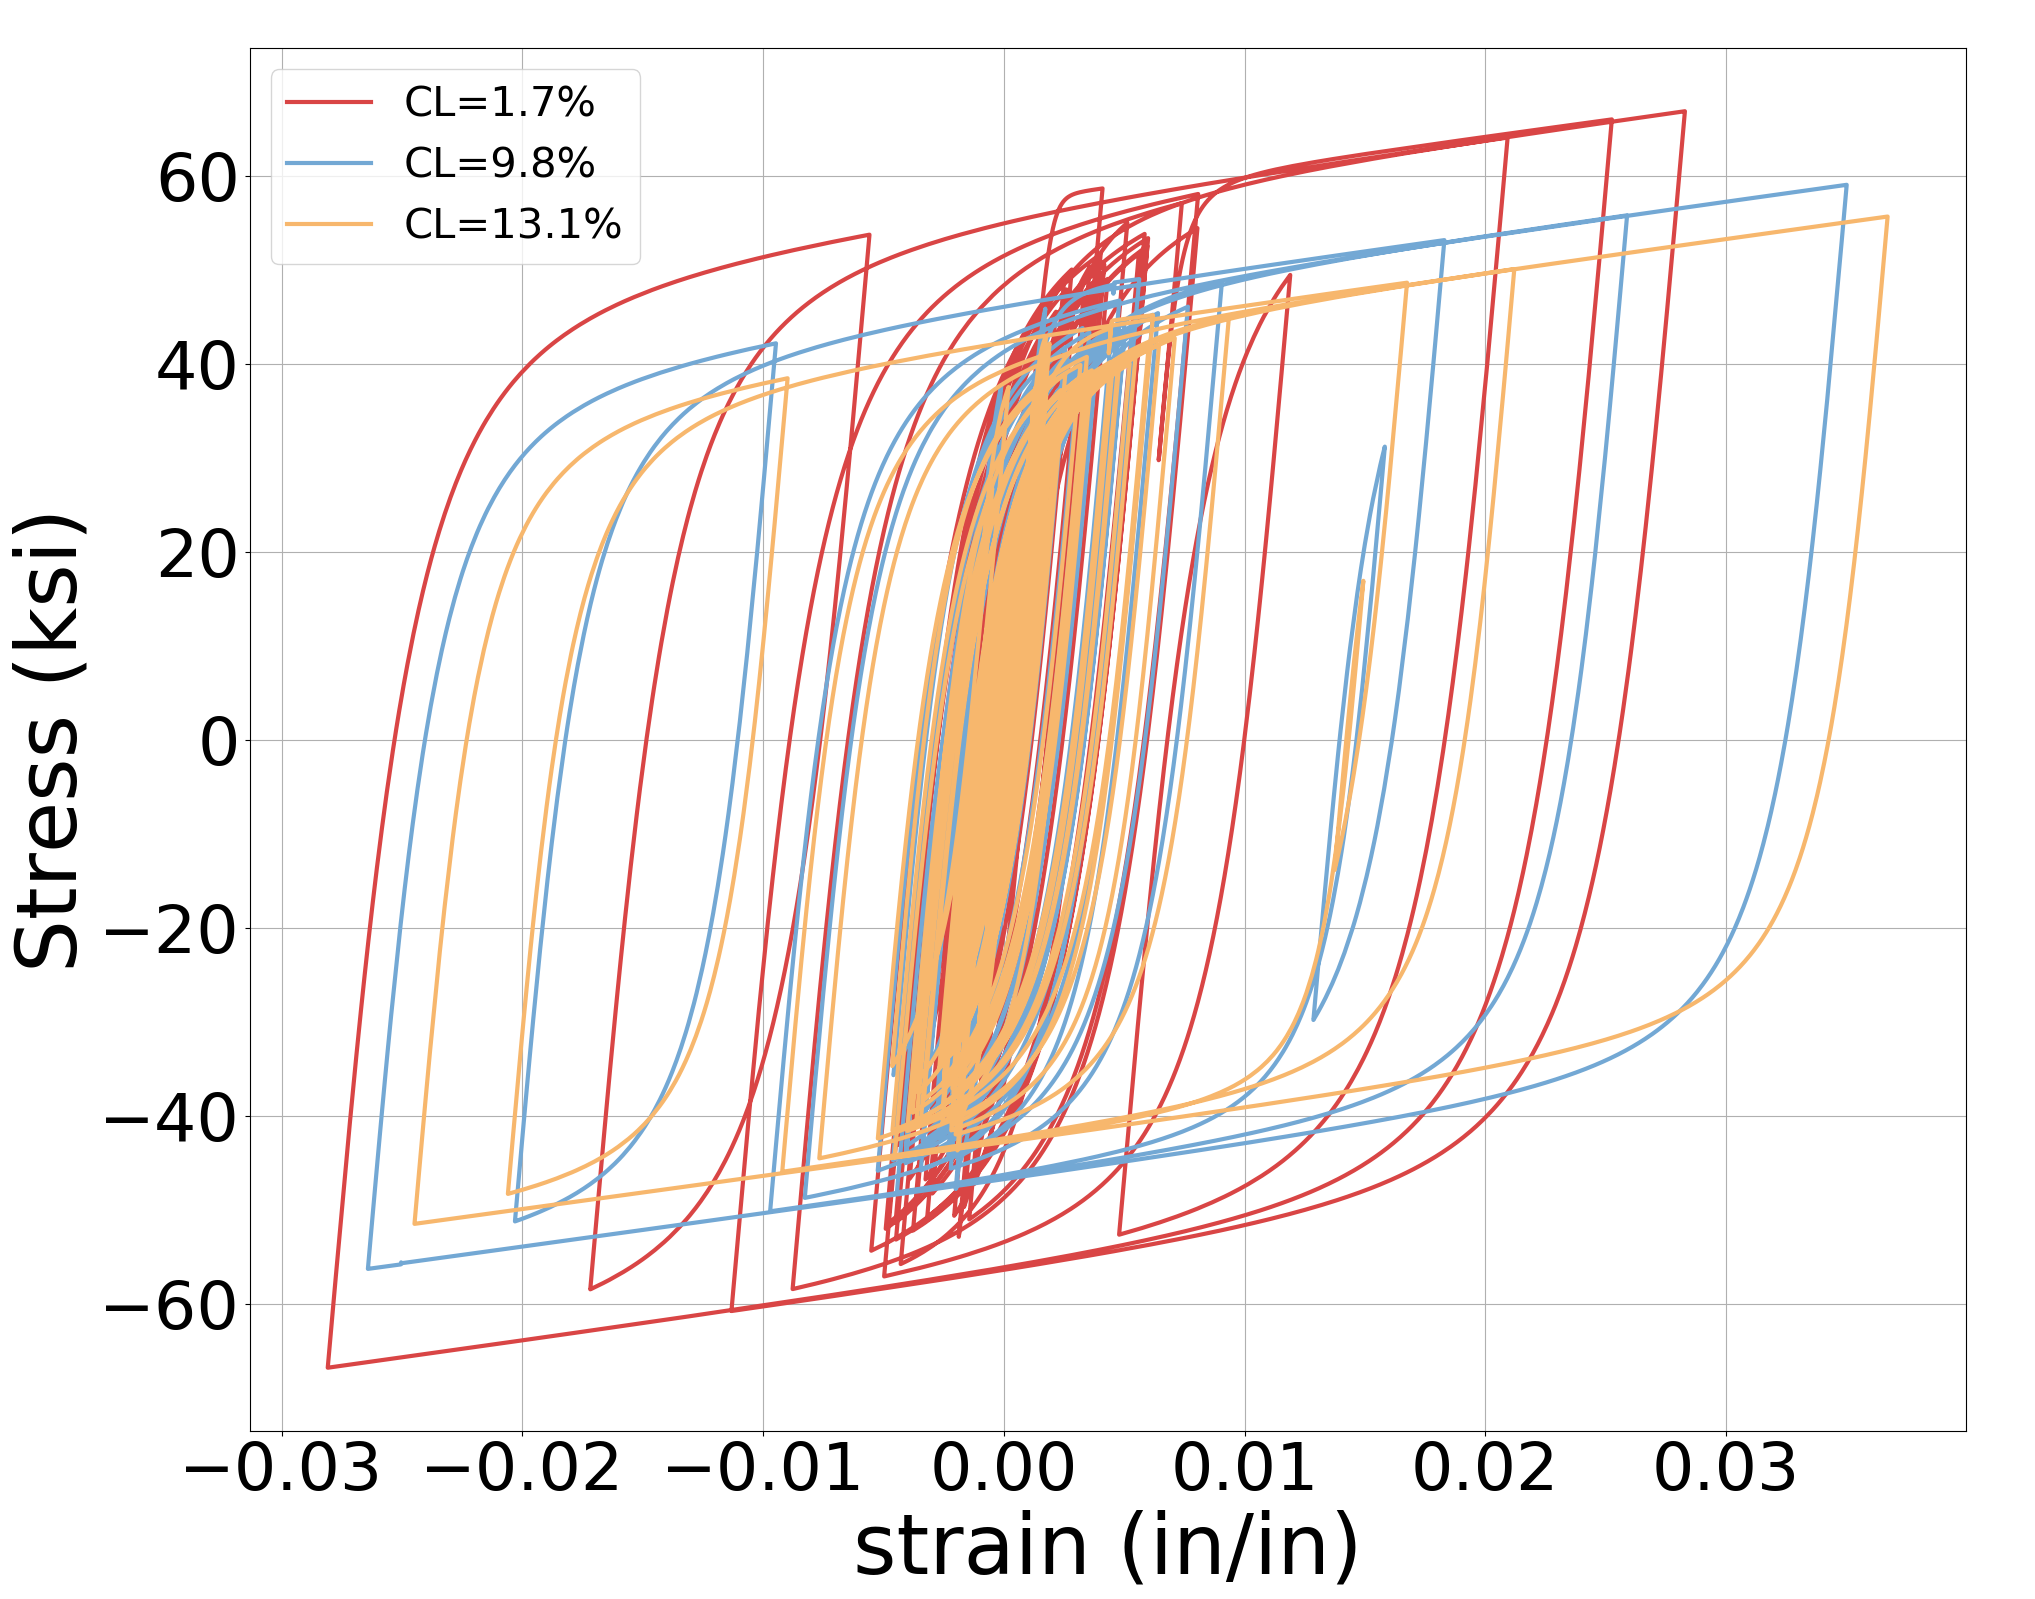
\includegraphics[width=0.65\textwidth]{Chapter-4/figs/Steel_StressStrain}
	\caption{Stress strain response for extreme rebar location}
	\label{fig:Steel_Stress_Strain_Response}
\end{figure}

\subsection{Development of cumulative distribution functions}

Once the analysis is complete the data is post-processed in a cumulative distribution function (CDF). The methodology employed corresponds to the multiple stripe analysis (MSA) recommended by Baker et al \cite{Baker2015}. While peak ground acceleration ($PGA$) has been widely used as the intensity measure to develop fragility functions\cite{Ghosh2015}\cite{Bisadi2015}\cite{Shekhar2018}, Krish \cite{Krish2018} in a recent study, showed that spectral displacement at first effective period ($IM=Sd(T_1)$) has better correlation than $PGA$. To demonstrate this, CDF curves were developed for $IM=PGA$ and $IM=Sd(T_1)$, and are shown in in figures \fref{fig:CDF_SY_PGA} and \fref{fig:CDF_SY_SDT1} correspondingly. The CDFs were developed for the steel yielding limit state, however this can be the extrapolated for any limit state. \fref{fig:CDF_SY_PGA} shows the results obtained with $IM=PGA$ do not show a good correlation since as corrosion increases the probability of exceeding a limit state decreases, this is not the behavior observed in \fref{fig:Steel_Stress_Strain_Response}. Conversely, \fref{fig:CDF_SY_SDT1} shows the results with $IM=Sd(T_1)$, these results present a better correlation, since, as corrosion increases, the probability of exceeding the limit state of yielding increases, for the preliminary results shown here the corrosion level of 13.1\% results are an exception. These results will improve as more analyses become available. 

\begin{figure}[htbp]
	\centering
	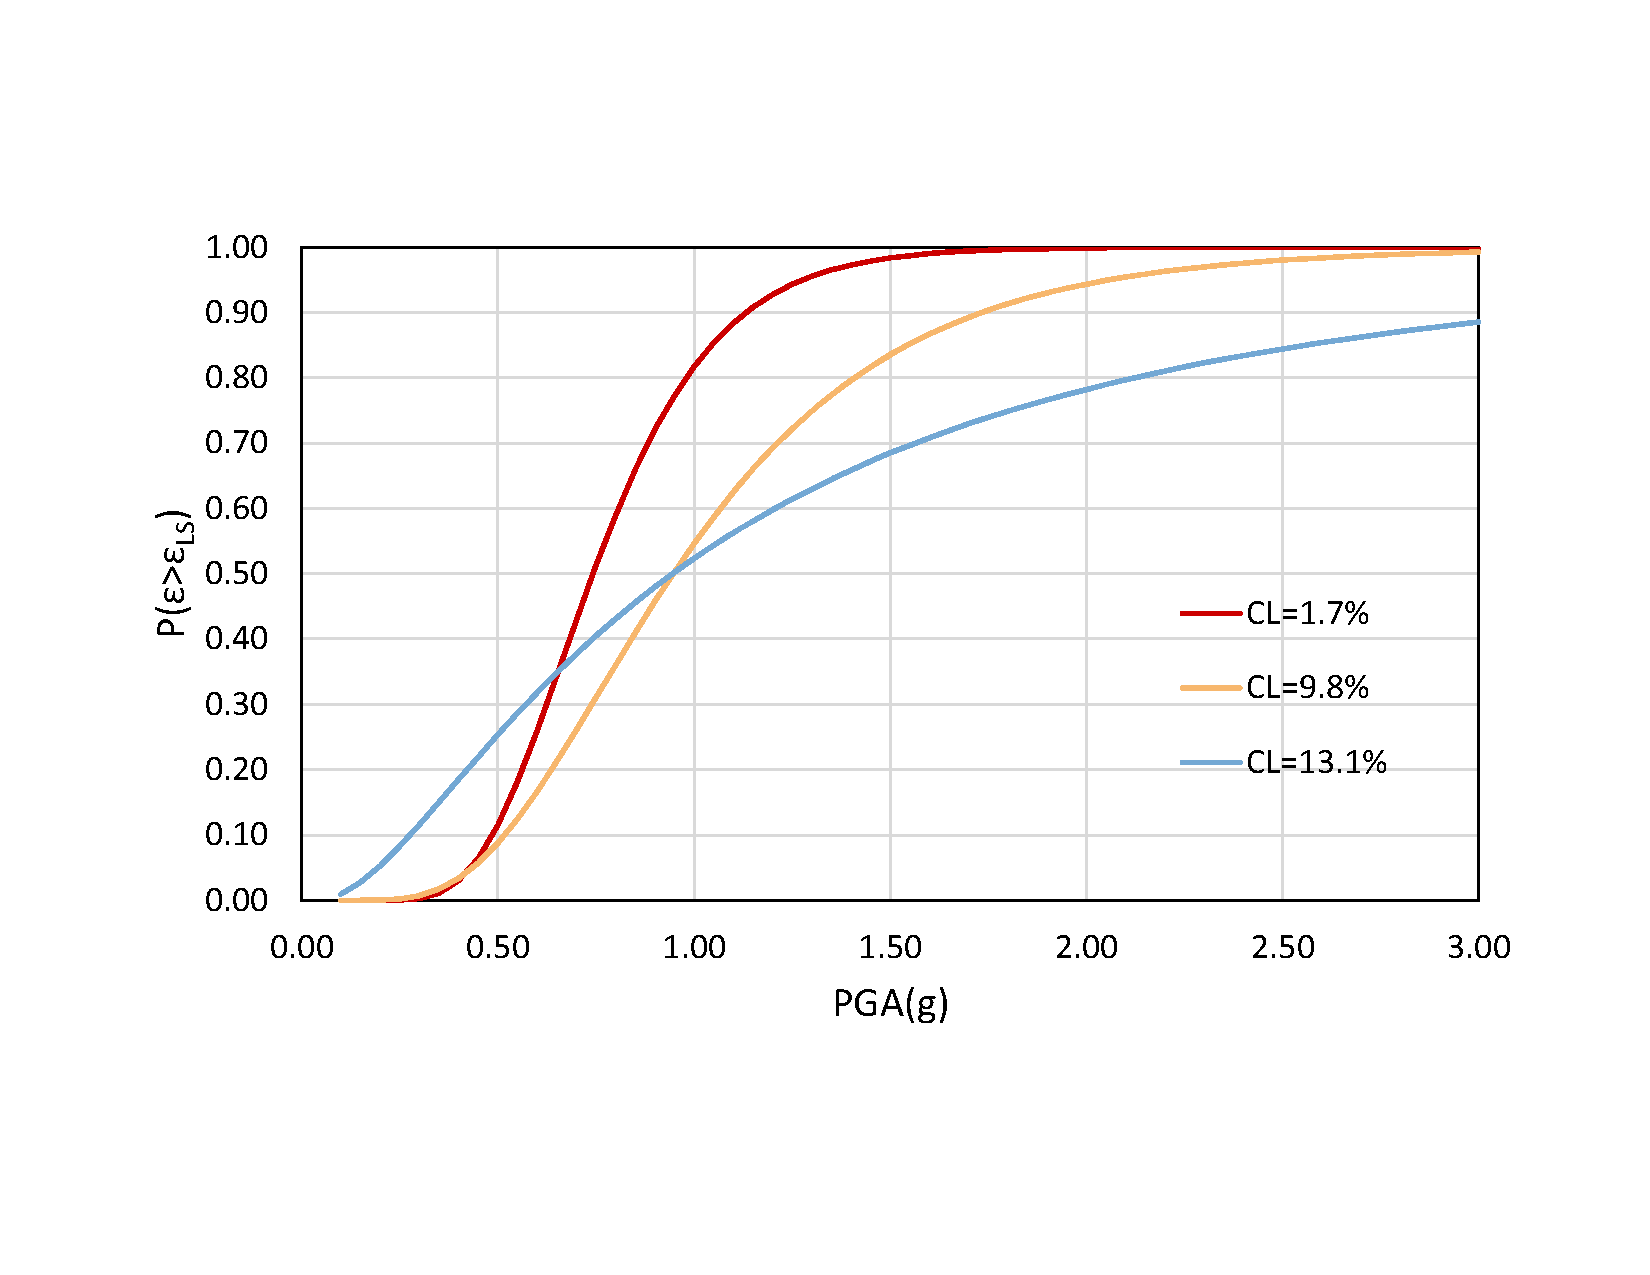
\includegraphics[width=0.8\textwidth]{Chapter-4/figs/CDF_PGA}
	\caption{CDF of steel yielding limit state using $IM=PGA$}
	\label{fig:CDF_SY_PGA}
\end{figure}
\begin{figure}[htbp]
	\centering
	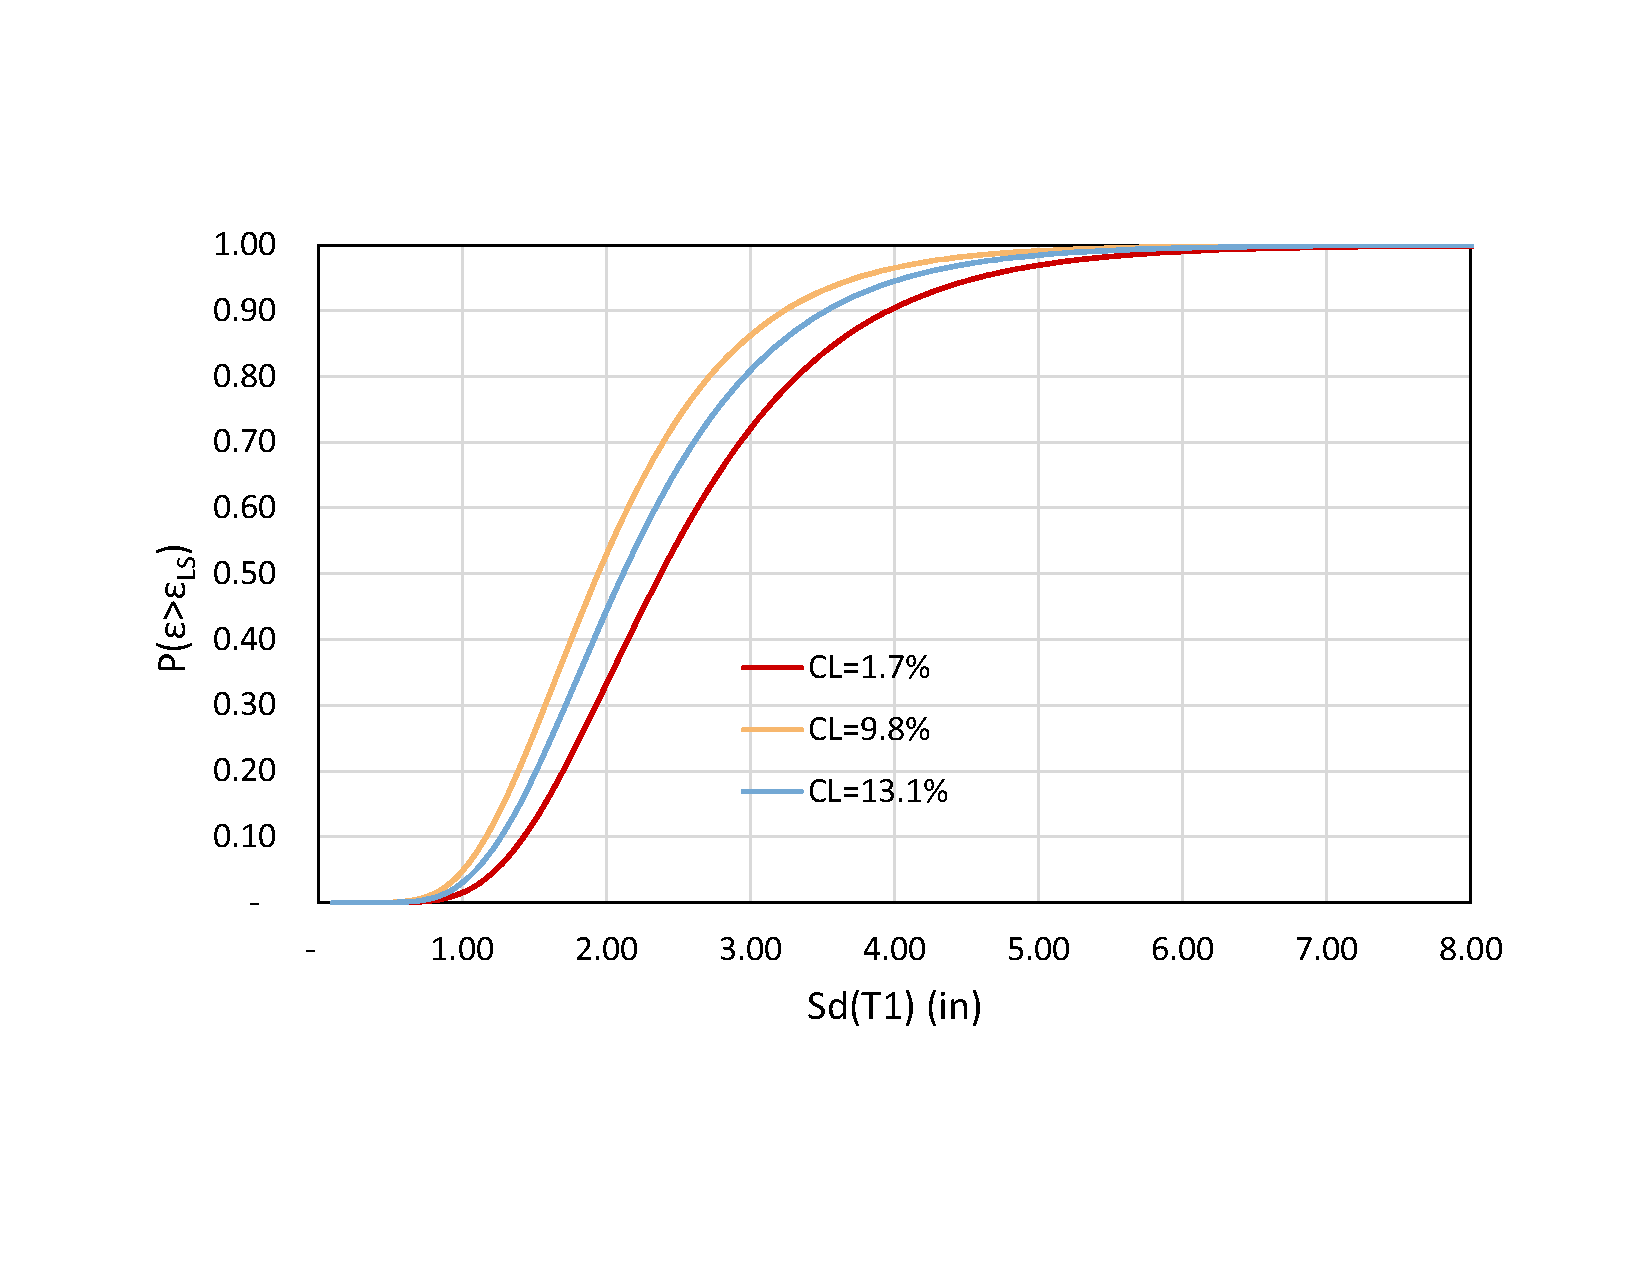
\includegraphics[width=0.8\textwidth]{Chapter-4/figs/CDF_SdT1}
	\caption{CDF of steel yielding limit state using $IM=Sd(T_1)$}
	\label{fig:CDF_SY_SDT1}
\end{figure}
\newpage
\subsection{Results discussion}
\begin{itemize}
	\item The results show that there is an increase in the demands as the corrosion in the structure increases. This is clearly shown in \fref{fig:CDF_SY_SDT1}. However, more results will help improve this correlation
	\item Results shown in \fref{fig:CDF_SY_PGA} and \fref{fig:CDF_SY_SDT1}, show that $IM=Sd(T_1)$ is a better intensity measure than $IM=PGA$
	\item The outcomes from the experimental campaign will further improve the results obtained in the analytical work
	\item The experimental phase will also provide an improved methodology to mimic the behavior of corroded reinforcing steel that is embedded inside the concrete
	\item The inclusion of additional aging conditions in the analysis will provide a realistic analysis of aging RC columns
\end{itemize}

\section{Future topics}

\begin{itemize}
	\item Concrete strength aging
	\item Welding and fatigue in steel structures
	\item Repair effects
	\item Main shock - after shock series - repair series
	\item Load history effects
	\item Degree of damage effect on confined structures behavior
	\item Selection of intensity measure (IM)
\end{itemize}

\chapter{Analytical Program}
\label{chap-five}
This research developed an analysis procedure that incorporated the effect of cumulative damage in RC structures. While previous studies have obtained results using the Ang and Park Damage Index and obtained fragility curves using the assumptions of that model, this research evaluated the performance of structures using strain limit states since strain limit state provides a better estimate of the level of damage sustained by structures during an earthquake. Therefore, an analytical model of an SDOF cantilever RC column was subjected to a series of nonlinear time history analyses (NLTHA) that considered aging conditions and sequences of mainshock and aftershock. The analytical model incorporated the effective mechanical properties found in the experimental program. 

The results from the analytical program showed that as recorded ground motion sequences did not increase, the maximum strain was achieved after a significant ground motion occurred. On the other hand, Corrosion level increased the demands and decreased the capacity of structures. Furthermore, the results show that as corrosion increases, reaching a given limit state also increases. These results determined that a maximum acceptable level of corrosion is CL=10\% which is congruent with the experimental program results.

\section{Modeling of corrosion for structural analysis}

The main objective of the analytical program is to determine the effects of corrosion on the demands of reinforced concrete columns. The results obtained in the experimental program have shown that corrosion affects the geometry of the surface of reinforcing steel bars by generating imperfections. The geometrical imperfections induced by the corrosion caused a reduction in the effective mechanical properties of the reinforcing steel material. The effective mechanical properties are a mathematical convenience to evaluate corroded RC structures. In general, as corrosion increases, the effective material properties of the steel decrease, as well as the average bar diameter.

In order to incorporate the effect of corrosion in the structural analysis, it is necessary to reduce the bar diameter and the effective mechanical properties of the reinforcing steel bar. For this study, uniform corrosion is the only type of corrosion considered. Therefore, assuming uniform corrosion, the diameter is reduced per the following expressions:

\begin{equation}
    d_{b,CL} = d_{b,o} \sqrt{1 - CL*0.01}
    \label{eq:d_eff}
\end{equation}

Where CL corresponds to the corrosion level, and $d_{b,CL}, d_{b,o}$ are the reduced diameter and the initial diameter correspondingly. 

Similarly, the mechanical properties of the reinforcing steel are modified with the expressions for effective yield and ultimate strengths found in the experimental program. The expressions proposed in Chapter \ref{chap-four} are replicated here for convenience:

\begin{equation}
    f_{y,CL} = f_{y,o}(1-0.0075CL)
    \label{eq.Calderon_Fy_vs_CL_5}
\end{equation}

\begin{equation}
    f_{u,CL} = f_{u,o}(1-0.0075CL)
    \label{eq.Calderon_Fu_vs_CL_5}
\end{equation}

\section{Multiple seismic events}

The evaluation of multiple seismic events is a topic that has been scarcely studied, however their effects have been felt in numerous earthquake sequences such as the Christchurch 2010, Umbria-Marche Earthquake 1997 and the Puerto Rico Earthquakes 2020. The hypothesis is that accumulation of damage will restart in a smaller seismic event to achieve a prescribed limit state, similar to how corrosion and other aging phenomena might impact the intensity needed to achieve a future limit state. 

For this study it was determined that not all damage in structures are dependent on multiple events but rather their condition when an event occurs as is the case for corrosion. Therefore, in this study a Mainshock-Aftershock (MS-AS) sequence is evaluated at different levels of corrosion.

\subsection{Earthquake selection}

The ground motions are taken from the NGA2 West Database of earthquake records provided by the Pacific Earthquake and Engineering Research Institute (PEER) \cite{Ancheta2014}. This database consists of 599 different earthquake events that characterize the ground motions on the west coast of the contiguous United States. To study the effect of mainshock and aftershock sequences, only records that had aftershocks recorded were used. In addition, the parameters shown below were also used to filter the database to ensure that the records would produce considerable ammounts of displacement.

\begin{itemize}
	\item Moment magnitude $M_w \geqslant 5$
	\item $PGA>0.04$
	\item $PGV>1$ cm/s
	\item $Vs_{30}>100m/s$ \& $Vs_{30}<1000$ m/s
	\item Lowest usable frequency is less than 1Hz
	\item $R_{rup}<60km$
\end{itemize}

Figure \fref{fig:GM_Selection} summarizes the results from filtering the data available in the PEER NGA West2 database. \fref{fig:GM_Selection} shows the earthquakes as moment magnitude {Mw} vs rupture distance ($R_{rup}$). In addition, the spectral displacement is an important intensity measure used in this study, therefore, the displacement spectrum for the ground motions used in this research are shown in \fref{fig:DisplacementSpectrum_Selection}. Figures \fref{fig:GM_Selection} and \fref{fig:DisplacementSpectrum_Selection}, show that there is a good level of variability between the records and provide a wide range of ground motion properties. 

\begin{figure}[htbp]
	\centering
	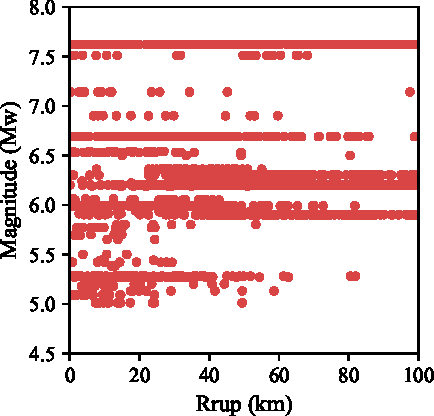
\includegraphics[width=0.45\textwidth]{Chapter-5/figs/GM_Selection.pdf}
	\caption{Mainshock selection from PEER NGA West2 database}
	\label{fig:GM_Selection}
\end{figure}

\begin{figure}[htbp]
	\centering
	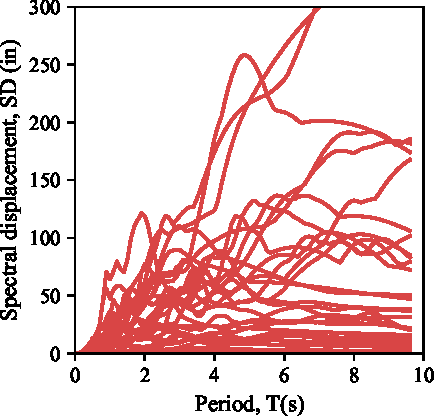
\includegraphics[width=0.45\textwidth]{Chapter-5/figs/SD_Spectrum_GM_Selection.pdf}
	\caption{Mainshock selection from PEER NGA West2 database}
	\label{fig:DisplacementSpectrum_Selection}
\end{figure}

\subsection{Modeling of mainshock-aftershock series for corrosion damage state}

Corrosion modifies the mechanical properties of rebars in RC structures, thus inherently modifying their response to earthquake loading. However, when an earthquake occurs is difficult to predict, as explained in section 2.4.2. Therefore, this study subjected structures with a specified corrosion level to a series of mainshock and aftershock ground motions. 
In order to analyze the structure to a sequence of mainshock and aftershock, it was necessary to glip together two ground motions. The process consisted of 1) selecting mainshocks and aftershocks from the same recording station and assigned to the same earthquake sequence, 2) the records were combined into a single file to run the sequence in order. The joined record also added a 4-second gap between the ground motions. This gap was to provide a sufficient amount of time for the record to reach stability. In contrast, the time to reach stability can vary depending on the structural and ground motion properties. A recommendation from Raghunandan et al. \cite{Raghunandan2015} found that 4s gives enough time for a structure to stabilize, a more significant time gap is possible, but it increases the computational cost significantly. An example of the resulting mainshock and aftershock sequence is shown in \fref{fig:MS-AS_sequence_sample}.

\begin{figure}[htbp]
	\centering
	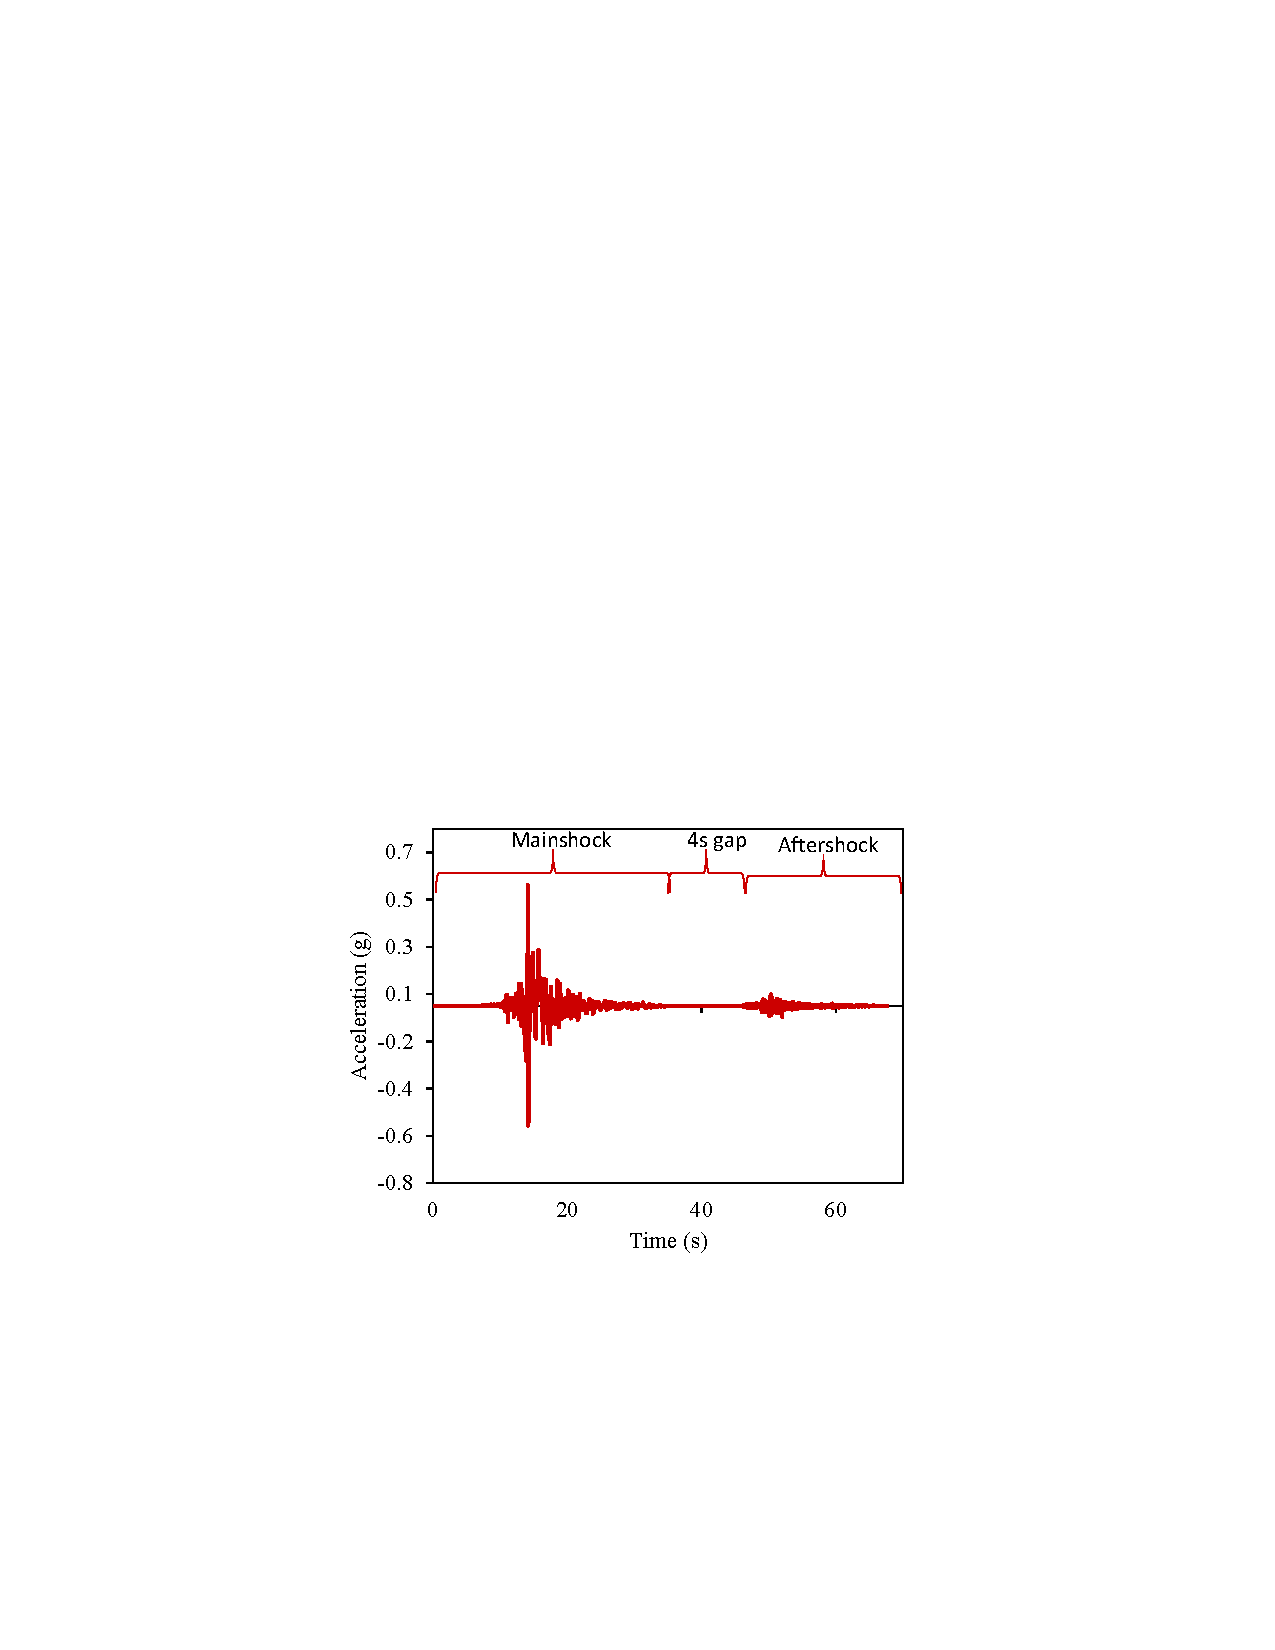
\includegraphics[width=0.6\textwidth]{Chapter-5/figs/MS_AS_Figure.pdf}
	\caption{Mainshock selection from PEER NGA West2 database}
	\label{fig:MS-AS_sequence_sample}
\end{figure}
\section{Analytical Model}
\subsection{Cantilever column}
This study focuses on the behavior of a single degree of freedom (SDOF) system representing a cantilever reinforced concrete column. The column is modeled as shown in \fref{fig:Structural_Model} This structure is modeled in OpenSeesPy \cite{McKenna2010}\cite{Zhu2018} using the $forceBeamColumn$ element \cite{Scott}. The forceBeamColumn element is used with two-point Gauss-Radau integration applied in the hinge regions and two-point Gauss integration applied on the element interior for a total of six integration points \cite{Scott}. The force-based formulation requires only a single element to accurately represent the full nonlinear deformation of the member and the integration scheme selected prevents the loss of objectivity during the softening response while also providing integration points at the member ends \cite{Calabrese2010},\cite{Scott}. The element requires the length of plasticity be defined at each end of the member, for which the tension-based rectangular plastic hinge length is calculated using the following expressions \cite{Goodnight2013}:

\begin{equation}
    L_{pc}=k*L_{eff} + 0.4D
    \label{eq:LP_Comp}
\end{equation}
\begin{equation}
	k=0.2*(Fu/Fy - 1) \leqslant 0.08
	\label{eq:K_Lp}
\end{equation}
\begin{equation}
    L_{pt}=L_{pc}+\gamma*D
    \label{eq:LP_Tension}
\end{equation}

For single bending the parameter $\gamma$ is:
\begin{equation}
    \gamma=0.33
    \label{eq:Gamma_LPt}
\end{equation}

The two-point Gauss-Radau integration is applied such that each end node integration is weighted equal to the specified plastic hinge length, as illustrated in \fref{fig:Fiber_PlasticHinge}. In this figure $D$ is the diameter of the column, and $c$ is the concrete cover. Therefore, strains recorded at the end sections represent accurate values even in the case where deformation localizes to the ends from strain-softening behavior. For the case of the cantilever column considered, only one plastic hinge length is defined, and the opposite end is given an arbitrary unit length. 

\begin{figure}[htbp]
	\centering
	\includegraphics[width=0.75\textwidth]{Chapter-5/figs/StructuralModel_01}
	\caption{Structural Model a) SDOF Column b) Structural Model}
	\label{fig:Structural_Model}
\end{figure}

\begin{figure}[htbp]
	\centering
	\includegraphics[width=0.9\textwidth]{Chapter-5/figs/fbc_PlasticHinge}
	\caption{End point plastic hinge method \cite{Scott}}
	\label{fig:Fiber_PlasticHinge}
\end{figure}

The cross section of the column is shown in \fref{fig:ColumnSection}. The column cross section is discretized with concrete and steel material fibers. Concrete fibers are modeled using the $Concrete01$ material, modified for confined material strength based on the Mander confined concrete model \cite{Mander1988}. The $Steel02$ material, based on the Giuffre-Menegotto-Pinto model \cite{Filippou1983} is used for the longitudinal reinforcement with recommended parameters ($b = 0.01, R0 = 20, cR1 = 0.925, cR2 = 0.15$). 

\begin{figure}[htbp]
	\centering
	\includegraphics[width=0.7\textwidth]{Chapter-5/figs/StructuralModel_Section}
	\caption{Section of the RC Column}
	\label{fig:ColumnSection}
\end{figure}
\subsection{Strain penetration}

The strain penetration considers the additional deformation due to anchorage of the reinforcement into the foundation, since tension strain in the reinforcement will drop to zero at a depth equal to the true development length of the rebar \cite{Priestley2007}. Experimental studies have generally reported that this end rotation contributes up to 35\% to the lateral deformation of flexural members\cite{Zhao2007}. Therefore, it is important to incorporate it into the analytical model. A way to capture this effect is by using a zero-length section element implemented in the nonlinear fiber-based analysis of concrete structures, which is available in the material library of OpenSeesPy as $Bond SP1$ \cite{Zhao2007}. This is the material model used for the steel fibers of the zero-length section element.

The required parameters for this model are:
\begin{itemize}
	\item $F_{y}$ Yield strength of the reinforcement steel
	\item $S_{y}$ Rebar slip at member interface under yield stress (see \eref{eq.Rebar_Slip})
	\item $F_{u}$ Ultimate strength of the reinforcement steel
	\item $S_{u}$ Rebar slip at the loaded end at the bar fracture strength a value of $35 S_{y}$ is recommended \cite{Zhao2007}
	\item $b$ Initial hardening ratio in the monotonic slip vs. bar stress response $b=0.45$ is recommended \cite{Zhao2007}
	\item $R$ Pinching factor for the cyclic slip vs. bar response $R=1.01$ is recommended \cite{Zhao2007}
	\item $d_b$ Rebar diameter
	\item $f'c$ Concrete compressive strength of the adjoining connection member
	\item $\alpha$ Parameter used in the local bond-slip relation and can be taken as $\alpha=0.4$ in accordance with CEB-FIP Model Code 90 \cite{CEB1993}
\end{itemize}.
\newline
Bar slip is calculated as:
\begin{equation}
	S_{y}(in)=0.1\left(\frac{d_{b}F_{y}}{4000\sqrt{f'_{c}}}\left(2\alpha+1\right)\right)^{\frac{1}{\alpha}}+0.013 (in)
	\label{eq.Rebar_Slip}
\end{equation}
\subsection{Design limit states}
Design limit states are defined based on strains in the material since they can more accurately represent the different performance levels. Structure limit states are tension strains in the rebars or compression strains in the concrete core. The values recommended in the typical performance-based design of reinforced concrete bridge columns are shown in Table  \ref{tab:DesignLimitStates}. The serviceability limit states correspond to the compression strain at which concrete cover begins to crush and the peak tension strain, resulting in residual crack widths of approximately 1 mm. These limits are generally accepted as nominal limit states for RC members. The compression limit state for damage control is defined by the expression shown in Eq. \ref{eq:ec_DamageControl}, and it refers to the compression strain in the confined concrete at which fracture of the transverse reinforcement confining the core occurs \cite{Priestley2007}. This equation is obtained using the strain-energy balance between that absorbed by the confined core concrete and the capacity of the confining steel. The damage control limit state is defined by the strain at the onset of buckling, which can be expressed according to \ref{eq:es_DamageControl}. This model demonstrated accurate predictions of the onset of bar buckling on physical tests in SDOF Concrete Column \cite{Goodnight2016}. An additional limit state is the ultimate limit state, proposed by Barcley et al. \cite{Barcley2019}, which is defined as the previous tension strain before bar fracture due to bar buckling. The limit state can be expressed as shown in \eref{eq:es_ultimate}. For the case of corrosion, the effective material properties of the reinforcing steel bars are used, and in the case of the ultimate limit state, the equation that relates corrosion and the maximum bending strain is used.

\begin{equation}
    \varepsilon_{c,spiral yield}=0.009-0.3\frac{A_{st}}{A_{g}} +3.9\frac{f_{yhe}}{E_{s}}
    \label{eq:ec_DamageControl}
\end{equation}

\begin{equation}
    \varepsilon_{s,BB}=0.03+700\rho_{s}  \frac{f_{yhe}}{E_{s}} -0.1\frac{P}{f'_{c}A_{g}}
    \label{eq:es_DamageControl}
\end{equation}
\begin{equation}
    \varepsilon_{t}=\frac{ln(\frac{\varepsilon_{b}}{0.001})}{\frac{300P}{f'c A_{g}}+\frac{0.7}{\rho_{t}}}
    \label{eq:es_ultimate}
\end{equation}

\begin{table}[htpb]
	\caption{Design limit states}
	\label{tab:DesignLimitStates}
        \begin{center}
        \begin{tabular}{lll}
        Limit State         & Concrete Limit State (in/in) & Reinforcing Steel Limit State (in/in) \\ \hline
        Serviciability      & 0.04                         & 0.015                                 \\ 
        Collapse Prevention & \eref{eq:ec_DamageControl}   & \eref{eq:es_DamageControl}             \\ 
        Fracture            & N/A                          & \eref{eq:es_ultimate}                   \\ 
        \end{tabular}
        \end{center}
\end{table}

\section{Comparison with existing physical tests}
The model used in this research is calibrated for the case of pristine conditions and the case of corroded columns. The calibration to a pristine condition column shows how reliable the results from the model are. Then the pristine condition model is modified with the corrosion model, as explained in section 4.1.1. The analytical model is compared to the results from the physical test on corroded RC columns. This will give confidence that the results obtained from the analytical model are reliable, and will be further enhanced with the experimental results.
\subsection{Pristine condition columns}
Goodnight et al performed a total of 30 circular RC columns quasi-static tests to evaluate strain limit states \cite{Goodnight2016}. From this set of tests, a sample of one was taken to calibrate the analytical model. The test performed by Goodnight et al on an SDOF cantilever column shows similar geometry to that presented in \fref{fig:Fiber_PlasticHinge}. The parameters used in this large scale test were: diameter $D = 24.0 inch$, height of the column $L = 8.0 ft$, yield strength of steel $f_{y} = 574.0 MPa$, ultimate strength of steel $f_{u} = 753.3 * MPa$, longitudinal steel volumetric ratio $\rho_{s} = 1.5\% $, transverse steel volumetric ratio $\rho_{v} = 1.0\% $, and strength of concrete at 8 days $f'_{c} = 39.8 MPa$.

The analytical model used these parameters to compare the results from the model to the experimental results. The results from the analysis show good agreement with the experimental results as evidenced in \fref{fig:ModelCalibration}. Thus, the results obtained from the model predict the overall system behavior and can be used to analyze other configurations of the structural model.
\begin{figure}[htbp]
	\centering
	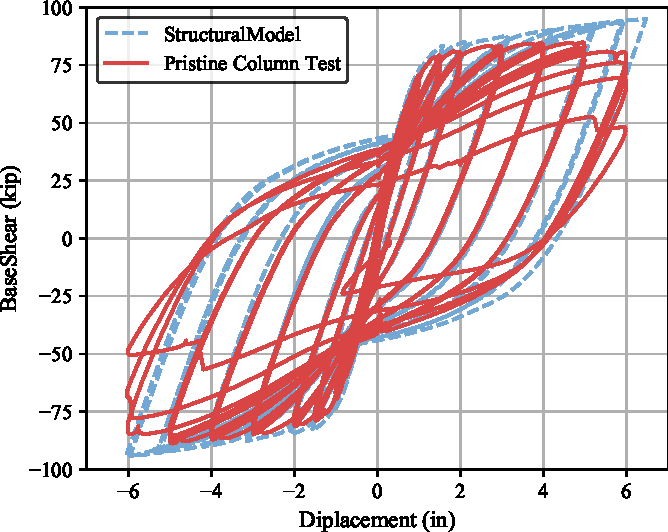
\includegraphics[width=0.60\textwidth]{Chapter-5/figs/Calibration_Test_26_Goodnight_et_al.pdf}
	\caption{Force-Displacement results from experimental results \cite{Goodnight2013} and analytical model}
	\label{fig:ModelCalibration}
\end{figure}

\begin{figure}[htbp]
	\centering
	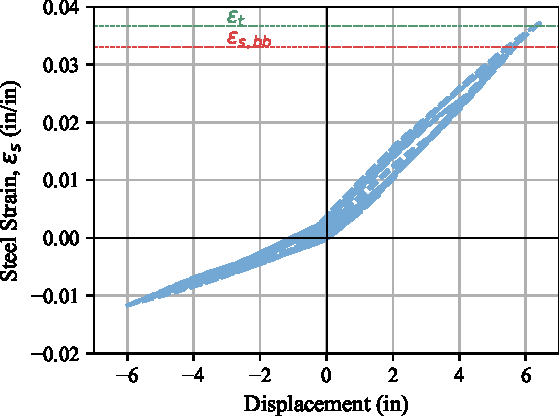
\includegraphics[width=0.5\textwidth]{VAC Thesis 2.0/Chapter-5/figs/Calibration_Test_26_Goodnight_et_al_strain.pdf}
	\caption{Strain hysteresis from experimental RC column in pristine condition}
	\label{fig:ModelCalibration_Pristine_Hysteresis}
\end{figure}

\subsection{Accelerated corrosion columns}
Similarly, Ma et al performed a series of quasi-static tests on RC columns with different corrosion levels and axial load ratios \cite{Ma2012}. From their study, the test with a corrosion level $CL=9.5\%$ was taken for calibration since the other tests presented in their study had excessively high axial load ratios which are not common in RC bridges. The results from Ma et al test	\cite{Ma2012} were used to compare against the analytical model. The column had the following parameters: diameter $D = 260.0 mm$, height of the column $L = 820.0 mm$, yield strength of steel $f_{y} = 375.0$ MPa, ultimate strength of steel $f_{u} = 572.3$ MPa, longitudinal steel volumetric ratio $\rho_{s} = 1.5\% $, transverse steel volumetric ratio $\rho_{v} = 1.0\% $, strength of concrete at 8 days $f'_{c} = 39.8$ MPa, and corrosion level $CL=9.5\%$. Equation \ref{eq.eleven} is used to modify the material properties of the reinforcing steel and considers the effects of corrosion. 

\begin{figure}[htbp]
	\centering
	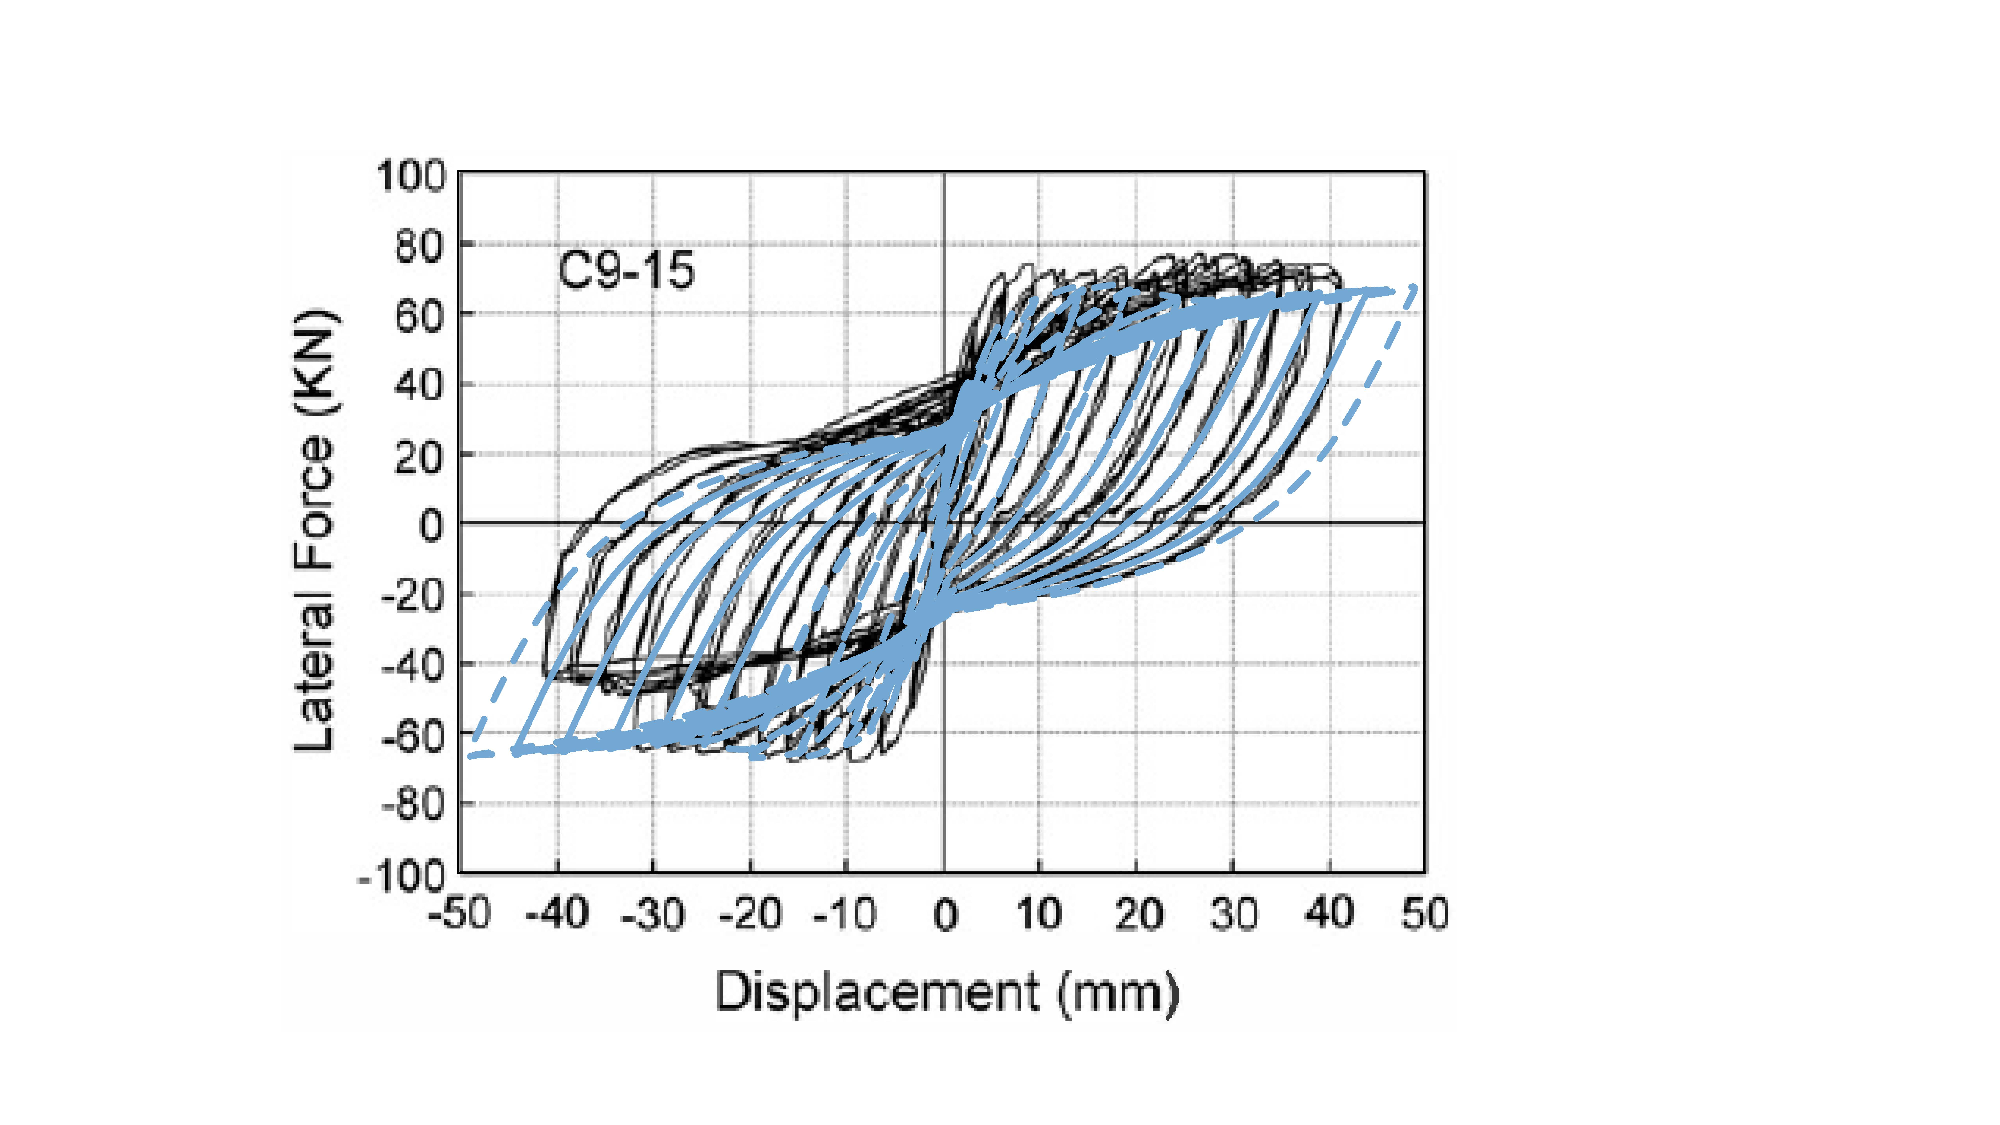
\includegraphics[width=0.50\textwidth]{Chapter-5/figs/Model_vs_MaEtAl_220218.pdf}
	\caption{Force-Displacement results from experimental RC column with corrosion in logitudinal bar (CL=9.5\%) \cite{Ma2012} and analytical model results (shown in lightblue)}
	\label{fig:ModelCalibration_Corrosion}
\end{figure}

Figure \ref{fig:ModelCalibration_Corrosion} shows that the results obtained from the analytical model capture the response of the structure with good accuracy. Ma et al \cite{Ma2012} did not report if bar buckling and bar fracture occurred during the test. However, the hysteresis curve shown in their study suggests that some damage limit state was reached. Therefore, \eref{eq:es_DamageControl} is used to determine the bar buckling limit state ($\varepsilon_{s,BB}=0.024$), this is then compared to the analytical model results shown \fref{fig:ModelCalibration_Corrosion_Hysteresis}. The results show a peak tension strain of $\varepsilon_{s}=0.023$, which is close to the value obtained using equation \eref{eq:es_DamageControl}. Therefore, there is a high likelihood that the bar buckling limit state was reached during this test. While these results are close, it is still not clear if \eref{eq:es_DamageControl} captures the behavior of the buckling limit state for corroded rebars. Thus, the proposed corroded BBT test will show if corrosion affects the behavior of buckled bars.

\begin{figure}[htbp]
	\centering
	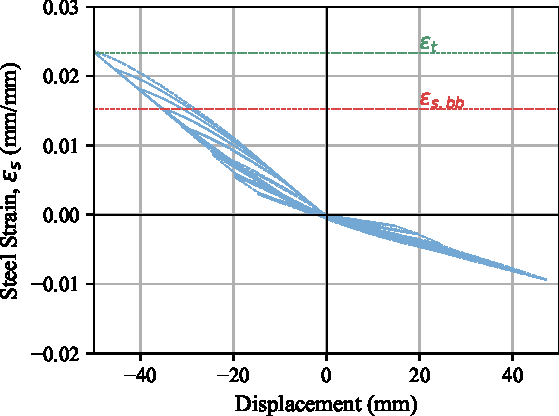
\includegraphics[width=0.5\textwidth]{VAC Thesis 2.0/Chapter-5/figs/Calibration_Ma_et_al_strain.pdf}
	\caption{Strain hysteresis from experimental RC column with corrosion in longitudinal bar (CL=9.5\%) results from analytical model}
	\label{fig:ModelCalibration_Corrosion_Hysteresis}
\end{figure}
\newpage
\section{Intensity Measure: $Sd(T_{eff},\xi)$}

When relating ground motions to structural response parameters, selecting appropriate quantities that accurately capture their relationship is crucial. Krish \cite{Krish2018} showed in a recent study that there is a good correlation between strain obtained from fiber modeling and first mode effective spectral displacement ($IM=Sd(T_1)$). On the other hand, peak ground acceleration $(PGA)$ did not correlate well. These conclusions are congruent with the results found by Mackie et al. \cite{Mackie2003}. 

In this study, the intensity measure was improved further by correlating the strains to the effective period of the structure $(T_{eff}$ and the equivalent damping $(\xi)$. These parameters are of substantial use in the Direct Displacement Based Design Methodology. The calculation of the effective period of the structure and the equivalent damping are explained below.

\subsection{Effective period calculation}

The process to calculate the effective period consists in obtaining first the effective stiffness of the structure. From the Non-Linear Time History Analysis (NLTHA) of a structure, the maximum displacement and force at the maximum displacement are obtained, as shown in \fref{fig:k_eff_calc}. With these values, the effective stiffness can be calculated as:

\begin{equation}
     K_{eff}=\frac{F(d_{max}}{d_{max}}
    \label{eq:Keff_calcualtion}
\end{equation}

\begin{figure}[htbp]
	\centering
	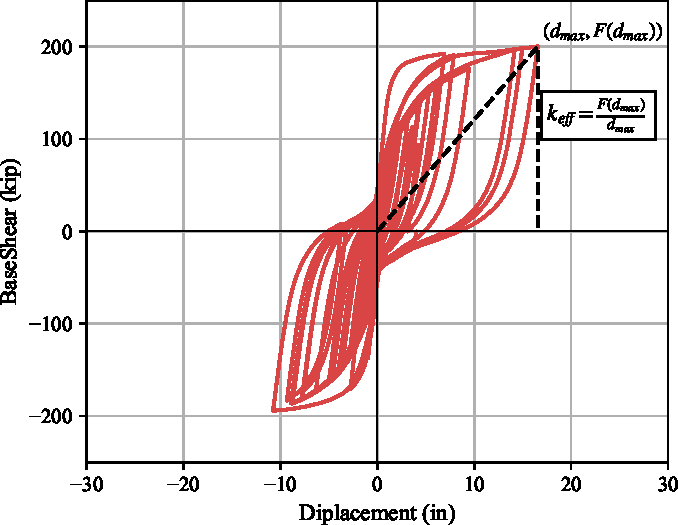
\includegraphics[width=0.60\textwidth]{VAC Thesis 2.0/Chapter-5/figs/Force_Diplacement_Keff_Calc.pdf}
	\caption{Calculation of effective stiffness $(k_{eff})$}
	\label{fig:k_eff_calculation}
\end{figure}

After obtaining the effective stiffness, the effective period can be calculated with the relationship for the period of a structure. The effective period is calculated as:

\begin{equation}
     T_{eff}=2\pi \sqrt{\frac{M}{K_{eff}}}
     
    \label{eq:Teff_calcualtion}
\end{equation}

In the analytical program the mass is calculated on the basis of the axial load applied to the structures. 

\begin{equation}
    M=\frac{P}{g}
    \label{eq:M_calcualtion}
\end{equation}

\subsection{Calculate $Sd(T_{eff},\xi)$}

After obtaining the effective period for each ground motion, it is possible to obtain the spectral displacement at 5\% damping for each ground motion for a given effective period. Finally, the equivalent damping that the system reached for a given ground motion must be found to obtain the spectral displacement at the effective period and equivalent damping. Using the expressions for equivalent damping from Priestley et al. for circular columns in bridges, the equivalent damping can be expressed as:

\begin{equation}
    \xi_{eq}=0.05+0.444\frac{\mu-1}{\mu\pi}
    \label{eq:EqDamping_calcualtion}
\end{equation}

The damping factor that corresponds to the equivalent damping is calculated as:

\begin{equation}
    DF=\sqrt{\frac{0.07}{0.02+\xi_{eq}}
    \label{eq:DF_calcualtion}
\end{equation}

Equations \eref{eq:EqDamping_calcualtion} and \eref{eq:DF_calcualtion} are part of the DDBD procedure outlined by Priestley et al \cite{Priestley2007}. Finally, the spectral displacement at effective period and equivalent damping can be expressed as:


\begin{equation}
    Sd(T_{eff},\xi)=DF Sd(T_{eff},5\%)
\end{equation}

The preceeding methodology can be seen graphically in \fref{fig:SpectralDisplacementCalculation}

\begin{figure}[htbp]
	\centering
	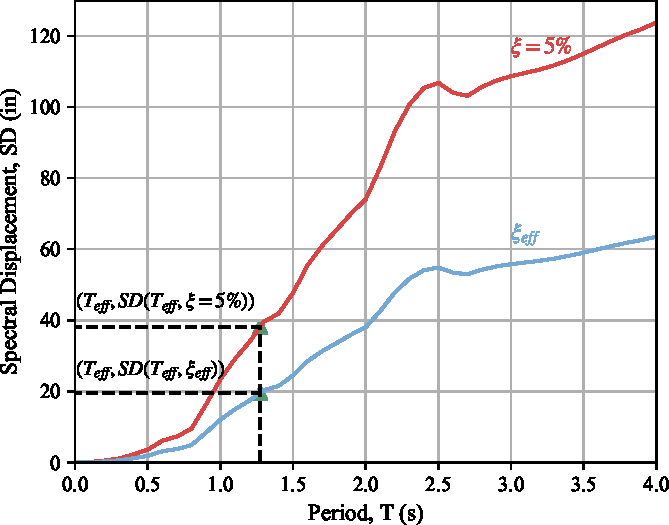
\includegraphics[width=0.6\textwidth]{VAC Thesis 2.0/Chapter-5/figs/SpectralDisplacement_SD(Teff,xi)_Calc.pdf}
	\caption{Calculation of spectral displacement at effective period at 5\% damping $Sd(T_{eff},5\%)$ and at equivalent damping $Sd(T_{eff},\xi)$}
	\label{fig:SpectralDisplacementCalculation}
\end{figure}

\section{Anlsysis of results using MSA}

Once the analysis is complete the data is post-processed and expressed as a cumulative distribution function (CDF). The methodology employed corresponds to the multiple stripe analysis (MSA) recommended by Baker et al \cite{Baker2015}. While peak ground acceleration ($PGA$) has been widely used as the intensity measure to develop fragility functions\cite{Ghosh2015}\cite{Bisadi2015}\cite{Shekhar2018}. Krish \cite{Krish2018} showed in a recent study, that spectral displacement at first effective period ($IM=Sd(T_1)$) has better correlation than $PGA$. To demonstrate this, CDF curves were developed for $IM=PGA$ and $IM=Sd(T_1)$, and are shown in \fref{fig:CDF_SY_PGA} and \fref{fig:CDF_SY_SDT1} respectively. The CDFs were developed for the steel yielding limit state; however this can be the extrapolated for any limit state. \fref{fig:CDF_SY_PGA} shows the results obtained with $IM=PGA$ do not show a good correlation since as corrosion increases the probability of exceeding a limit state decreases. This is not the behavior observed in \fref{fig:Steel_Stress_Strain_Response}. Conversely, \fref{fig:CDF_SY_SDT1} shows the results with $IM=Sd(T_1)$. These results present a better correlation, since, as corrosion increases, the probability of exceeding the limit state of yielding increases. For the preliminary results shown here, the corrosion level of 13.1\% results are an exception. These results will improve as more analyses become available. 

\begin{figure}[htp]
	\centering
	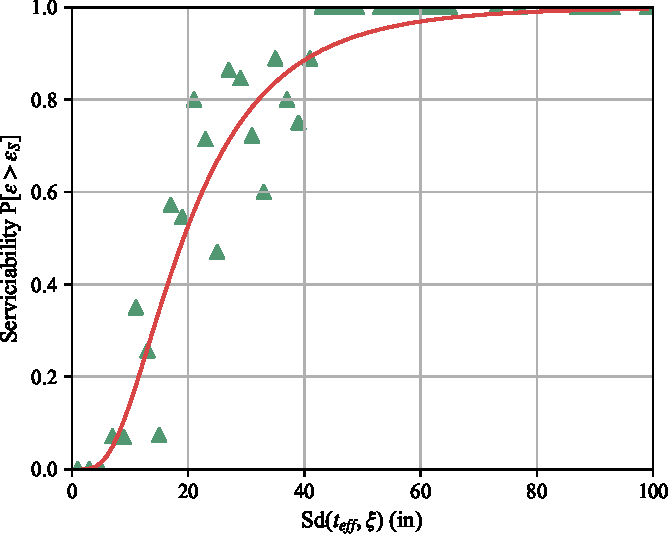
\includegraphics[width=0.60\textwidth]{VAC Thesis 2.0/Chapter-5/figs/MSA_Calc.pdf}
	\caption{MSA analysis}
	\label{fig:msa_sample_01}
\end{figure}

\section{Analytical framework}

The analytical framework was established to obtain the change in the structure performance due to aging conditions and to evaluate the effect of seismic events on the strain performance of single degree of freedom columns. This framework consisted of a program that performed and analyzed a series of nonlinear time history analyses (NLTHA). From these analyses, it was then possible to determine the effects of damage in the performance of structures. The proposed analytical framework process consisted of:

\begin{enumerate}
	\item Geometrical properties of the SDOF column 
	\item The effective mechanical properties of the reinforcing steel were evaluated.
	\item Nonlinear time history analyses of discrete ground motions and sequence of ground motions
	\item Posprocessing of data
\end{enumerate}

The analysis matrix for the corrosion aging phenomenon that was analyzed in this study is shown in Table \ref{tab:AnalysisMatrix}. The area or extent covered in the analysis corresponds to the range of variables that are common for RC columns in bridges.These analysis matrix resulted in a total of 36,000 analysis for the discrete ground motion analysis and 96,000 analysis for the sequences of ground motion case. To perform this large volume of analysis the Henry2 High Performance Computer (HPC) was used, to run the analysis in parallel. 

\begin{table}[htb]
	\caption{Analysis matrix}
	\label{tab:AnalysisMatrix}
	\centering
\begin{tabular}{{lcc}}
Parameter                          & Parameter        & Range                  \\	\hline
Diameter of column                     & D                & 28-90 in               \\	
Column aspect ratio        & L/D              & 4-8                    \\	
Longitudinal ratio                     & $\rho_s$         & 0.01-0.04              \\	
Axial load ratio                       & ALR              & 5\%-20\%               \\	
Corrosion level                         & CL               & 0\%-20\%               \\	
\end{tabular}
\end{table}

\subsection{Analysis Algorithm}

In order to run the analysis efficiently, a program was developed to perform three main routines:
1) Main program: setting conditions, the geometry of the model, effective material properties, 2) Run the Non-Linear Time History Analysis, 3)Post-processing of data

The main program is shown in \fref{fig:main_flowchart}. This program has three main inputs the ground motion records, the geometry of the column, and the aging conditions, which correspond to the corrosion level, the initial material properties, the axial load ratio, and the aspect ratio. After the inputs are done, a nested loop that goes through the different parameters is performed. The basic flow consists of preparing the data into the NLTHA subroutine and the post-processor subroutine. Once the program goes through the subroutines, the data output from OpenSees is deleted to use the HPC resources efficiently. This process is repeated until all the variables have been evaluated and the program finishes.

\begin{figure}[htp]
	\centering
	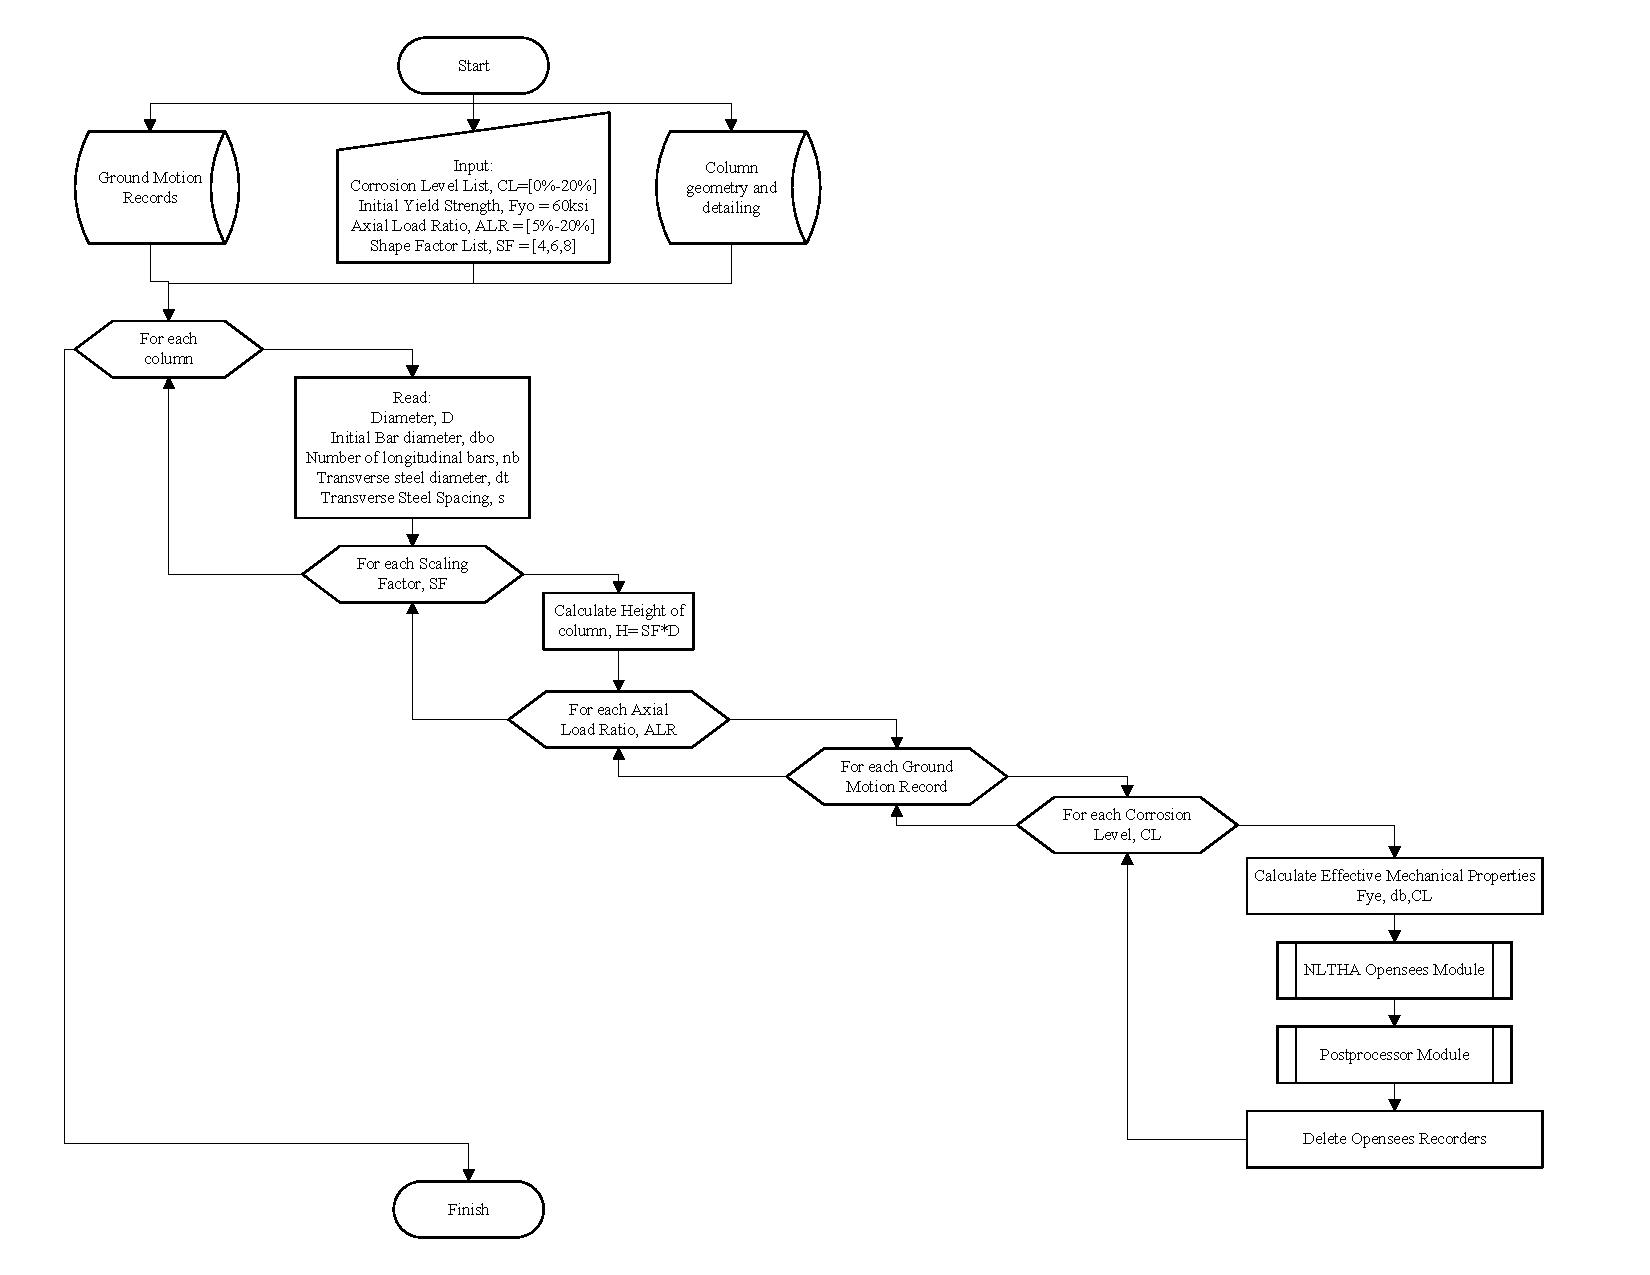
\includegraphics[width=0.975\textwidth]{VAC Thesis 2.0/Chapter-5/figs/Main_FlowChart_01.pdf}
	\caption{Main Flow-Chart}
	\label{fig:main_flowchart}
\end{figure}

The NLTHA subroutine consisted of a sequential process as shown in \fref{fig:nltha_flowchart}. First, the geometry of the model is established as per the model shown in \fref{fig:Structural_Model}. Then the material properties and the cross-sectional fibers are defined. Next, the recorders that store the analysis results throughout the NTLHA are set. Then the axial load is run and kept constant through the analysis. Finally, the NLTHA is run until it finishes.

\begin{figure}[htp]
	\centering
	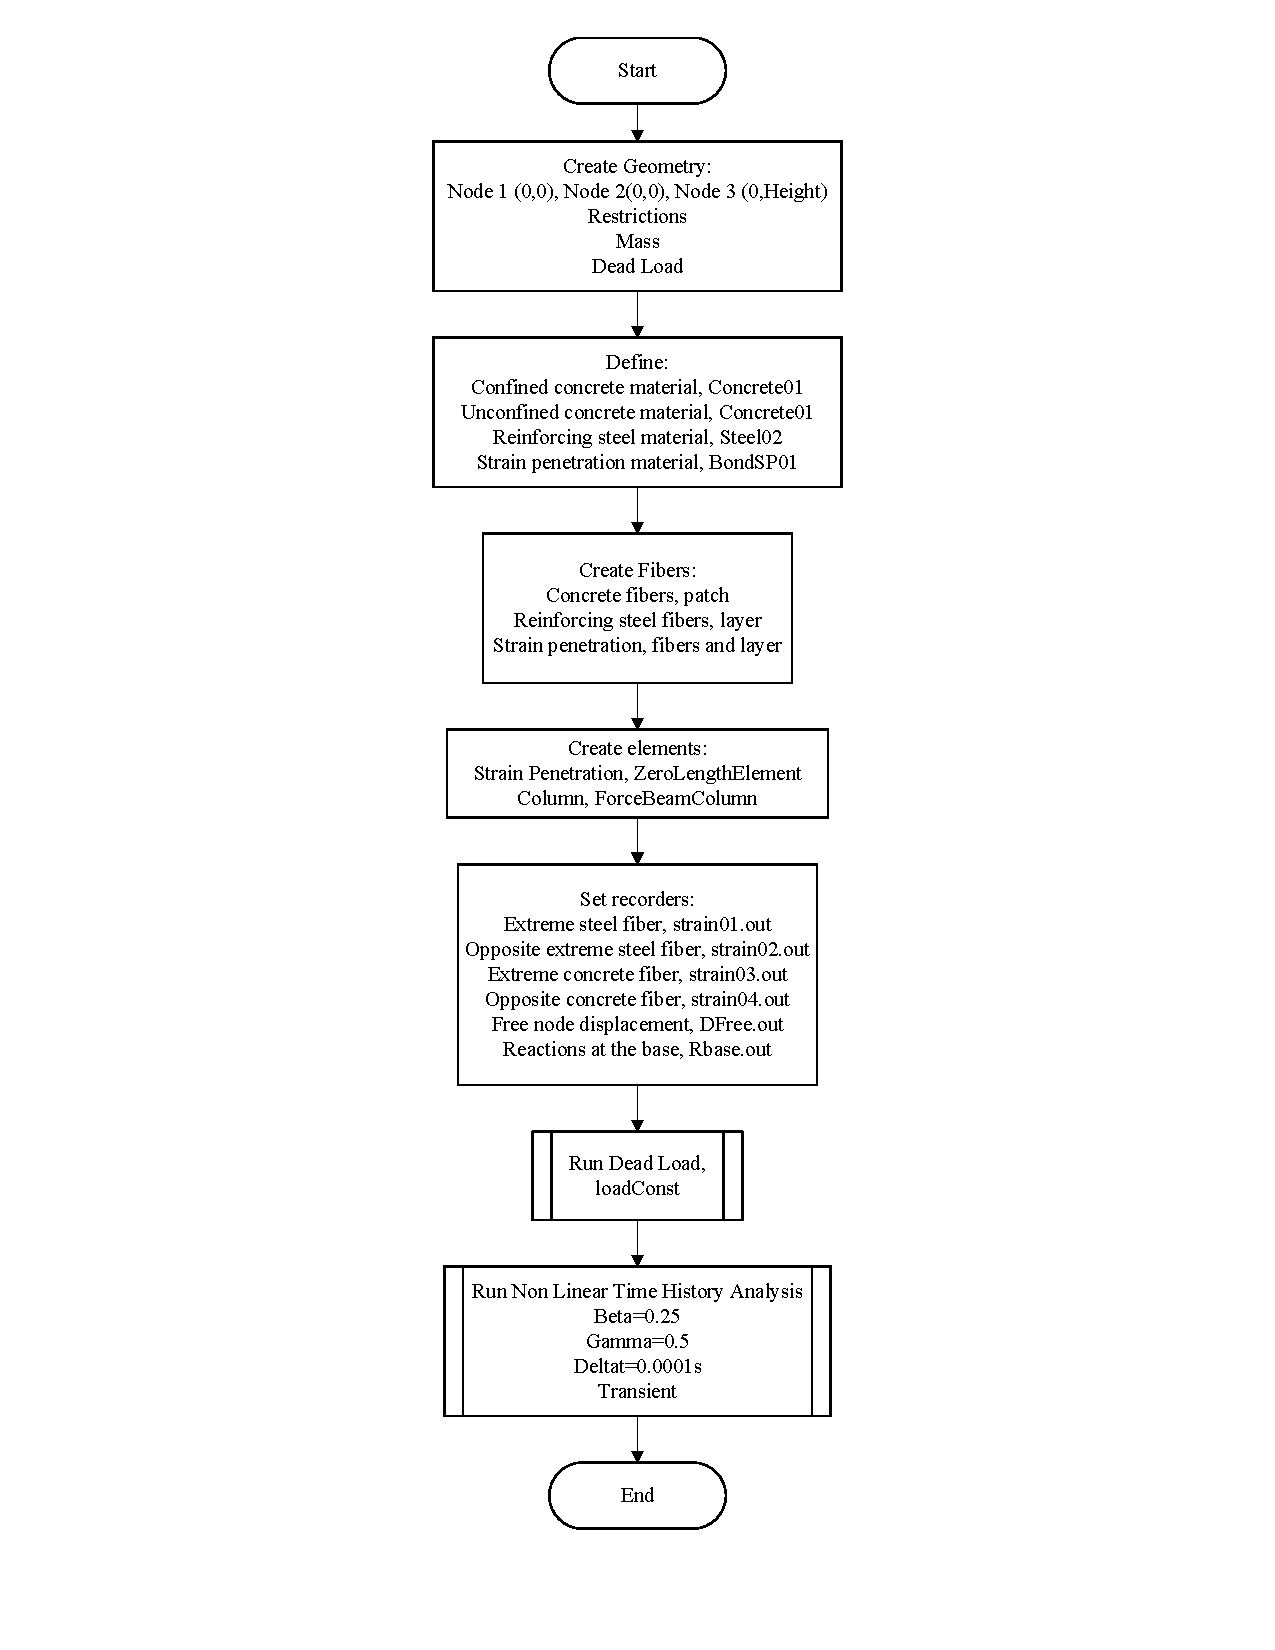
\includegraphics[width=0.425\textwidth]{VAC Thesis 2.0/Chapter-5/figs/NLTHA_FlowCharts_01.pdf}
	\caption{NLTHA Flow-Chart}
	\label{fig:nltha_flowchart}
\end{figure}

The post-processor subroutine also consisted of a sequential process as shown in \fref{fig:postproc_flowchart_01} and \fref{fig:postproc_flowchart_02} . The main goal of this subroutine is to store the data related to the model, including the geometry and material properties used in the analysis. The post-processor calculates the limit states as explained in section 5.3.3. Then the spectral displacement at the effective period is calculated for the ground motion following the procedure explained in section X.X. Finally, a collapse analysis for each limit state is performed in order to perform the multi-stripe analysis explained in the following section, all the relevant data is then stored in a database for further analysis.

\begin{figure}[htp]
	\centering
	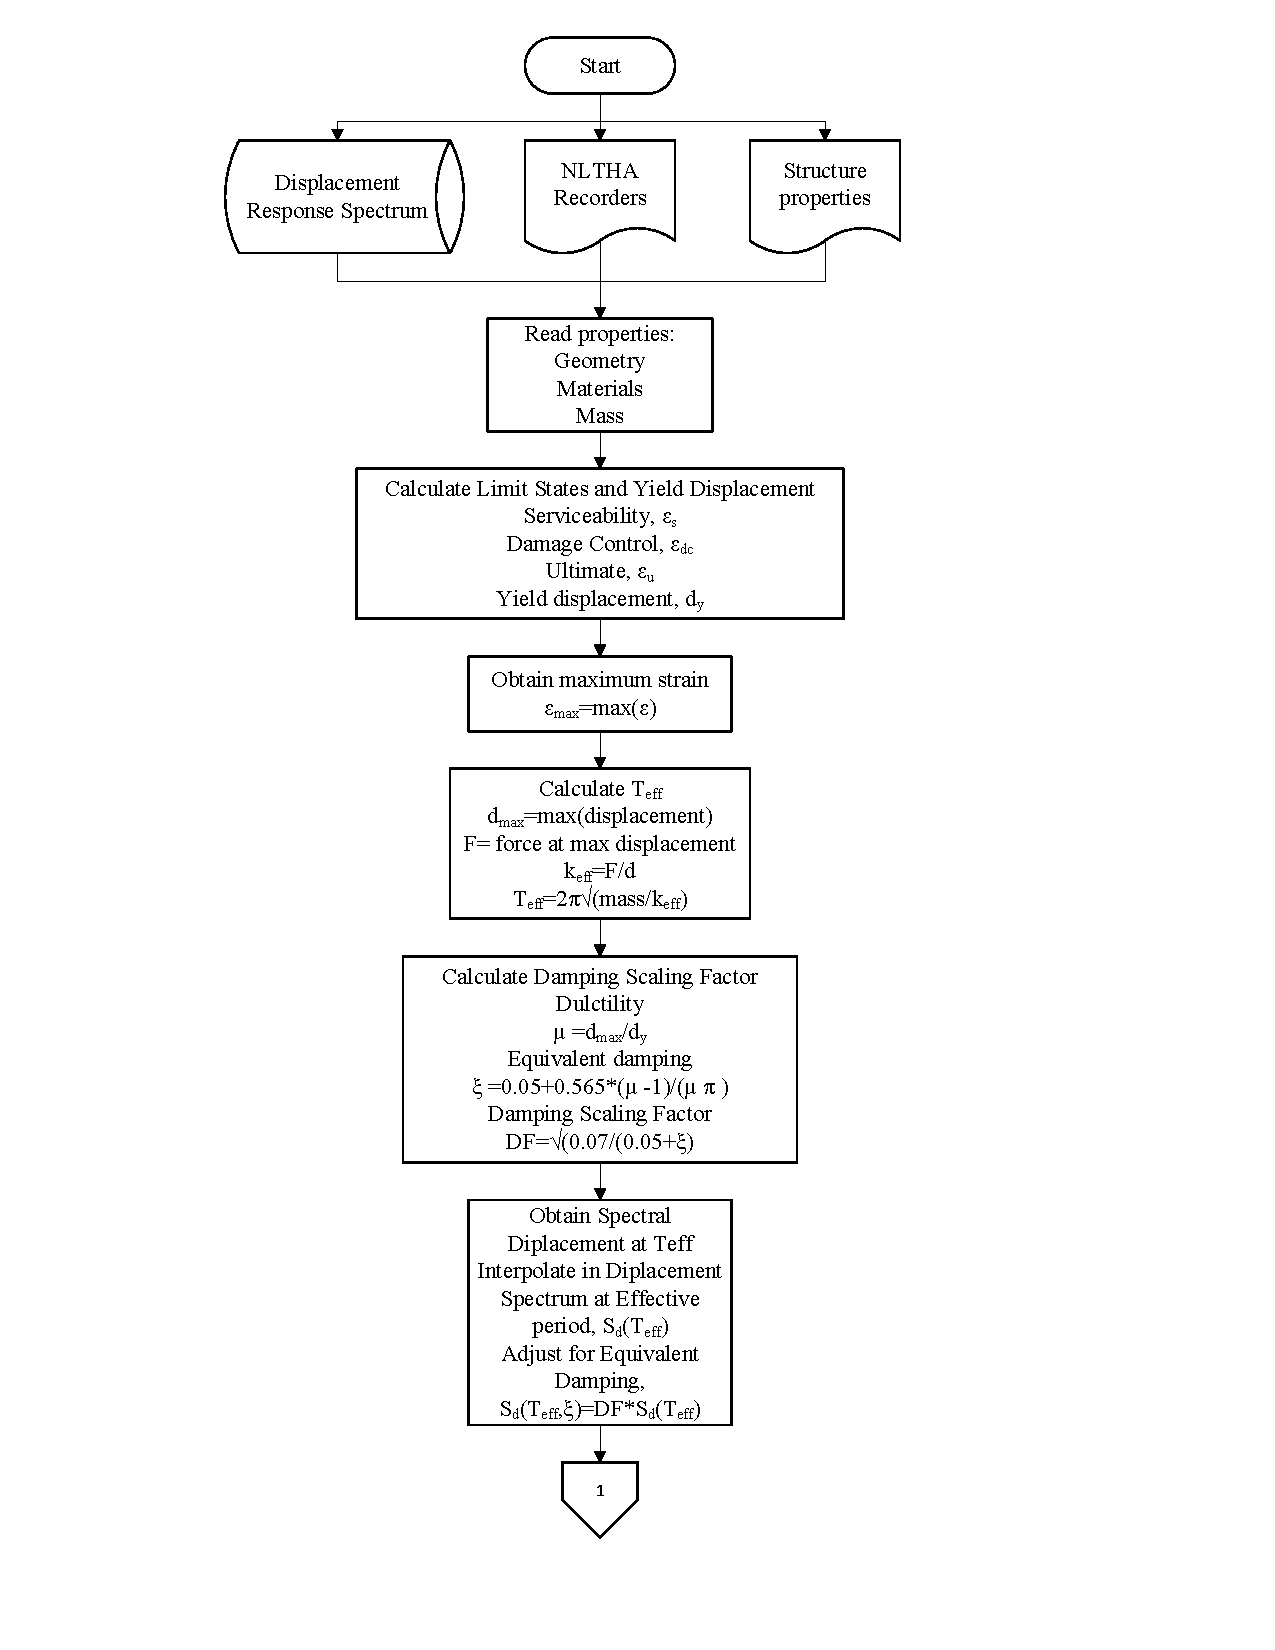
\includegraphics[width=0.575\textwidth]{VAC Thesis 2.0/Chapter-5/figs/PostProcessor_FlowCharts_01.pdf}
	\caption{Post-processor Flow-Chart}
	\label{fig:postproc_flowchart_01}
\end{figure}

\begin{figure}[htp]
	\centering
	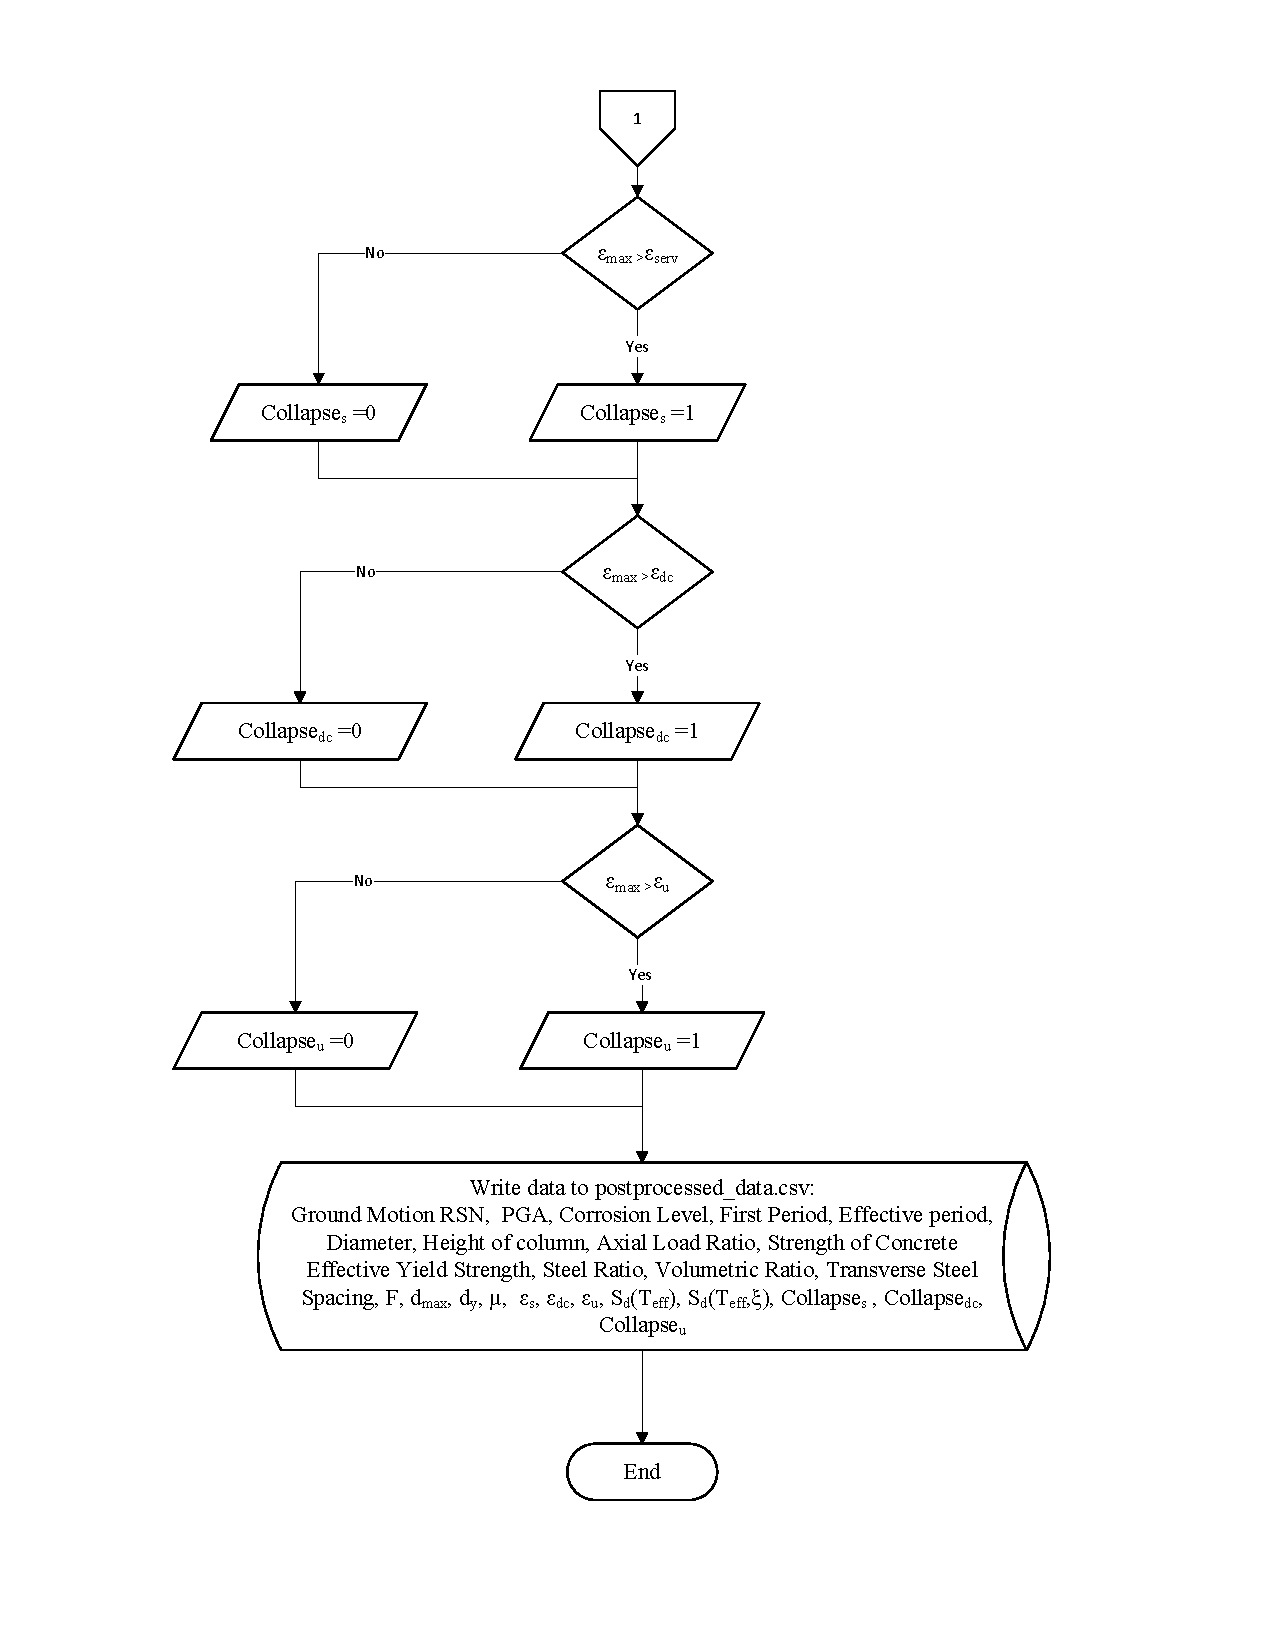
\includegraphics[width=0.75\textwidth]{VAC Thesis 2.0/Chapter-5/figs/PostProcessor_FlowCharts_02.pdf}
	\caption{Post-processor Flow-Chart continued}
	\label{fig:postproc_flowchart_02}
\end{figure}




%This procedure has been summarized in the form of a flow chart presented in \fref{fig:NLTHA_Framework}
%
%\begin{figure}[htbp]
%	\centering
%	\includegraphics[width=0.9\textwidth]{Chapter-5/figs/AnalysisFramework_01}
%	\caption{Analysis Framework Flowchart}
%	\label{fig:NLTHA_Framework}
%\end{figure}
%
%\section{Earthquake selection}
%\lipsum[4]
\section{Results from Analytical Program}
This section presents the results obtained from a non-linear time history analysis (NLTHA) performed using OpenSeesPy \cite{Zhu2018}. The structure was subjected to a total of 18 earthquake records. The primary responses obtained from these analyses correspond to the maximum strain obtained for the different levels of corrosion. The structure was analyzed for a range of corrosion levels [1.5\%-13\%] in the longitudinal rebars.

\subsection{Structural Response at Different Corrosion Levels}
Figures \ref{fig:Force-Displacement_Results} and \fref{fig:Steel_Stress_Strain_Response} are presented as an example of the results obtained using NLTHA. These results are extracted from the structure's response to the Chi-Chi earthquake. \fref{fig:Force-Displacement_Results} shows the global system response and \fref{fig:Steel_Stress_Strain_Response} shows the stress-strain response of the extreme fiber of reinforcing steel. These results show that as corrosion increases, the demands imposed on the structure increase too. Therefore, the probability of reaching a limit state increases as corrosion increases.

\begin{figure}[htbp]
	\centering
	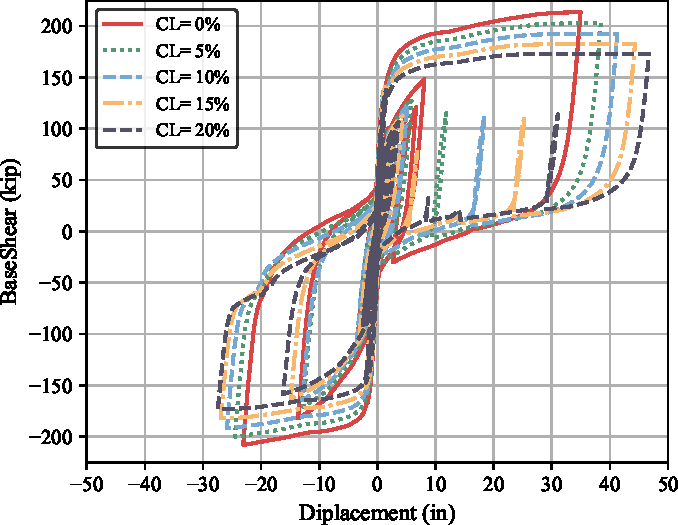
\includegraphics[width=0.7\textwidth]{Chapter-5/figs/Force_Diplacement_RSN1505.pdf}
	\caption{Force-Displacement results}
	\label{fig:Force-Displacement_Results}
\end{figure}

\begin{figure}[htbp]
	\centering
	\includegraphics[width=0.7\textwidth]{Chapter-5/figs/Stress_Strain_RSN1505.pdf}
	\caption{Stress strain response for extreme rebar location}
	\label{fig:Steel_Stress_Strain_Response}
\end{figure}

\begin{figure}[htbp]
	\centering
	\includegraphics[width=0.7\textwidth]{Chapter-5/figs/Diplacement_Strain_RSN1505.pdf}
	\caption{Strain hysteresis}
	\label{fig:Steel_Stress_Strain_Response}
\end{figure}

\subsection{Effect of groundmotion sequences}

\begin{figure}[htbp]
	\centering
	\includegraphics[width=0.65\textwidth]{VAC Thesis 2.0/Chapter-5/figs/MS_AS_results_noincrease_in_demands.pdf}
	\caption{Non Linear Time History Analysis (NLTHA) results showing no increase in the strain demands due to as recorded mainshock-aftershock sequence}
	\label{fig:ms_as_results}
\end{figure}

\subsection{Effect of corrosion level on Strain demands $(\varepsilon)$}

The strain demands $(\varepsilon)$ were plotted against the spectral displacement at the effective period and the equivalent structure damping ($Sd(T_{eff},\xi)$). These two parameters seem to have a linear correlation for all the corrosion levels evaluated. These results are shown in \fref{fig:all_results_nltha}

\begin{figure}[htbp]
	\centering
	\includegraphics[width=0.65\textwidth]{VAC Thesis 2.0/Chapter-5/figs/All_results_NLTHA_Figure.pdf}
	\caption{Non Linear Time History Analysis (NLTHA) results for Strain demands vs Spectral Displacement at Effective Period $(T_{eff})$, and Equivalent Damping $(\xi)$}
	\label{fig:all_results_nltha}
\end{figure}

The multi-stripe analysis(MSA) was used to obtain a series of cumulative distribution functions to evaluate the effect of corrosion and other variables. The most impactful variables are the corrosion level and the axial load ratio. The effect of these variables are shown in \fref{fig:CDF_strain_vs_ALR}. These figures show that as corrosion level increases, the mean spectral displacement required to preclude a given limit state is decreased. Similarly, the effect of the axial load ratio becomes substantial as it increases.

\begin{figure}[htbp]
	\centering
	\includegraphics[width=0.9\textwidth]{VAC Thesis 2.0/Chapter-5/figs/CDF_summary.pdf}
	\caption{Cumulative Distribution Function (CDF) for steel strain limit states and different Axial Load Ratios (ALR)}
	\label{fig:CDF_strain_vs_ALR}
\end{figure}

In order to observe the effect of corrosion level and axial load ratio, the mean spectral displacement, defined ad the point where the probability of reaching a limit state is 50\% ($P(\varepsilon>\varepsilon_{ls}=0.5$), is plotted against these two variables. The results are shown in \fref{fig:mean_prob_vs_CL}.

From the results shown in \fref{fig:mean_prob_vs_CL}, two main tendencies can be observed. First, as corrosion level increases, the mean spectral displacement required to reach a limit state decreases, thus precluding an earlier limit state in a corroded structure. It also appears that there is a significant drop at a corrosion level of 10\% ($CL=10\%$), especially for the damage control limit state and the ultimate limit state. This result indicates that a corrosion level this high has potentially undesirable consequences. Research performed on RC members has shown that corrosion levels of 10\% are brittle. Thus, these results are congruent with those observations.

The second observation is that Axial Load Ratios (ALR) greater of 10\% and higher have a more significant drop in their performance due to corrosion. This ALR value is commonly found in bridges, thus the importance of limiting the corrosion level that bridge columns develop in their service years.

\begin{figure}[htbp]
	\centering
	\includegraphics[width=0.85\textwidth]{VAC Thesis 2.0/Chapter-5/figs/Analysis_of_Mean_SDs.pdf}
	\caption{Analysis of mean values $(P=0.5)$ for performance limit states}
	\label{fig:mean_prob_vs_CL}
\end{figure}

The results obtained from these analyses are essential since they provide limiting values for the level of corrosion that could be acceptable in new structures and assessment of existing structures. Therefore, a limiting value for the level of corrosion in new designs should be between 0\%-5\%. For existing structures, a maximum acceptable level of corrosion could be set at $CL=10\%$. This recommendation is made because existing structures would not have been designed to account for aging or corrosion inhibitors. These existing structures would have to consider the effective properties and reduce the cross-section of the reinforcing steel bars. 

Further studies on limit states of corroded structures while improving the outcomes here identify and improve the design and assessment of RC members.

\subsection{Discussion of results}

The Nonlinear Time History Analysis results show that, in general, there is an increase in the strain demands due to corrosion. The increase in the strain demands depends on the limit state being evaluated and the axial load ratio. 

For all limit states, a corrosion level of 10 percent is a reasonable estimate of the maximum acceptable corrosion level. This result agrees with observed behavior in large-scale tests conducted on RC members. An ideal maximum level of corrosion is a 5\% corrosion level.

A limitation of this study was the use of limit state equations based on pristine condition elements with modern detailing. While the limit state equations provide the overall effect of corrosion in RC structures, future studies will provide more information on limit states for aged structures with and without modern detailing.

Therefore, the analytical program agrees with observed experimental material tests conducted as part of this research and observations on corroded RC member tests. Thus, for the design of new structures, it is recommended that an acceptable level of corrosion range is 5\%-10\%. Moreover, for assessment, it is recommended that if a corrosion level greater than 10\% is found, an NLTHA must be performed to assess the existing structure. This analysis will have to consider the effective mechanical properties of the reinforcing steel and the reduction in the cross-sectional properties. These recommendations are applied in the following chapter. 

Another interesting finding was that the effect as recorded sequences of mainshock-aftershock appears negligible. This result is in agreement with previous studies performed on MDOF systems that included degradation of the system in steel frames \cite{Ruiz-Garcia2011}. However, other studies that rely on altered records obtain the opposite result because they change the frequency content of their records.
\chapter{Condition Dependent Performance Based Design and Assessment}

\label{chap-six}

In this chapter, the experimental and analytical program results are used for two application examples. Two examples of the design and assessment of bridges that consider their corrosion is shown.

In addition, the existing methodologies to design structures for life service and assessment for existing structures are evaluated. As will be seen, these methodologies provide tools to consider aging in the structures. However, none of these methodologies directly evaluate corrosion in the structural analysis and design of the structure. Therefore, this study proposes a design and assessment methodology for a single degree of freedom for RC columns subjected to corrosion.

\section{Design of new structures for condition dependent PBD}

One of the biggest challenges in Civil Engineering is to provide infrastructure that is resilient, affordable, and safe. Currently, the design approach assumes that the material properties will remain unchanged throughout the life of the structures. However, built structures age and deteriorate and could potentially lead to the unintended consequence of a structure failing due to aging. Therefore, it is of interest to ensure that new structures are designed to perform to an acceptable level of performance and maintain the level of performance as the structure ages. \fref{fig:ConditionDependent PBD} shows the concept of condition-dependent performance-based design versus the traditional design approach. 

\begin{figure}[htbp]
	\centering
	\includegraphics[width=0.9\textwidth]{VAC Thesis 2.0/Chapter-6/figs/CD_DDBD_Concept.png}
	\caption{Philosophy of Condition Dependent Performance Based Design}
	\label{fig:ConditionDependent PBD}
\end{figure}

Currently, existing methodologies provide probabilistic frameworks to design structures for aging. While these methodologies have been used in recent years for significant bridge projects such as the Samuel de Champlain Bridge and the New Bonner Bridge, there is a gap in determining the level of performance as the structure deteriorates.

\subsection{Acceptable level of corrosion for new designs}

The experimental program obtained the equations that relate the degradation of the yield strength and maximum bending strain with corrosion. It was also noticeable in the experimental results that for corrosion levels of 10\% and greater, the bar's strength and capacity to sustain significant buckling levels were significantly reduced. Similarly, the corrosion levels of 10\% and greater in the analytical program significantly increased the likelihood of reaching the damage control and ultimate limit states. Therefore, it becomes evident that for design, a level of corrosion less than 10\% is acceptable for the design of new structures, although a level of corrosion of 5\% or less is desirable.

\subsection{Life Service Design Existing methodologies}

\subsubsection{Life 365}

The Life 365 Consortium III developed the software Life365 to estimate the service life and life-cycle costs of alternative concrete mixture designs and corrosion protection systems\cite{Bentz2003}. The software uses probabilistic analyses of the service life of reinforced concrete structures. The software can calculate the probability distributions within a known time when reinforcement corrosion initiation is expected to occur for a structure. In addition, representative values of the variability of the parameters used in the analysis are provided, such as average temperature throughout the year, Corrosion concentration limits, type of environment (Tidal zone, Spray zone, 800m from the ocean, 1.2 km from the ocean), the type of structure (Parking garage, Urban highway, Rural highway). One of the assumptions is that the deterioration time after corrosion initiation is constant at six years. This program makes it practical to use such distributions in making engineering judgments regarding selecting reinforcement corrosion protection strategies and considering the life costs of different designs. In this study Life 365 is used to accurately determine the time of initiation of corrosion. An example on how the different environments affect the corrosion process is shown in \fref{fig:Life_365_example}.

\begin{figure}[htbp]
	\centering
	\includegraphics[width=0.6\textwidth]{VAC Thesis 2.0/Chapter-6/figs/Life365.pdf}
	\caption{Life 365 corrosion level for 100 years of life service in different environments}
	\label{fig:Life_365_example}
\end{figure}
\subsubsection{FIB 34 Model Code}
FIB 34 model code addresses Service Life Design (SLD) for plain concrete, reinforced concrete, and pre-stressed concrete structures, focusing on design provisions for managing the adverse effects of degradation. Its objective is to guide bridge stakeholders, practicing engineers, and contractors to ensure that the condition of the bridge components and materials are kept above a minimum acceptable level throughout the structure's lifespan. With new bridges having requirements to last for at least 100 years, the design of structures that consider the life service variable has become ever more critical. Therefore, it is crucial to consider one of the primary aging conditions that affect bridges, such as corrosion.

Four different options for SLD are avilable in FIB 34:
\begin{enumerate}
    \item Full probabilistic approach,
    \item Semi probabilistic approach (partial factor design),
    \item Deemed to satisfy rules
    \item Avoidance of deterioration.
\end{enumerate}

An application of the FIB 34 model code has been implemented in a design guide developed by the Federal Highway Administration (FHWA) and the  American Association of State Highway and Transportation Officials (AASHTO) to implement a Service Life Design for Bridges (also referred to as R19A) through the second Strategic Highway Research Program (SHRP2)\cite{SHRP22019}. Multiple tools, products, and training materials aimed at practitioners and state bridge engineers were developed for the implementation effort. In SHRP2-R19A, FIB 34 with a fully probabilistic approach is used to design bridges. The design must ensure that the corrosion is reduced to a 10\% probability of occurrence. In addition, the methodology is implemented to different parts of the structure with exposure zones assigned to them, as shown in \fref{fig:FIB_34_Exposure zones}. Based on the reliability obtained, changes in the mix design, the reinforcing steel, the cover, and other variables can be made to increase the reliability of the structure. 

\begin{figure}[htbp]
	\centering
	\includegraphics[width=0.6\textwidth]{VAC Thesis 2.0/Chapter-6/figs/SHRP_exposure_example.jpg}
	\caption{Example of identification of exposure zones according to SHRP-R19A \cite{SHRP22019}.}
	\label{fig:FIB_34_Exposure zones}
\end{figure}


This methodology provides a probabilistic methodology to reduce the likelihood of corrosion throughout the structure's life. However, the methodology does not provide a way to directly consider the effect of corrosion on the structure's performance as it ages. Therefore, to ensure that the bridge's condition remains above a minimum acceptable level, it is necessary to evaluate the structure's performance at a given acceptable level of corrosion. The reliability check process is shown in \fref{fig:FIB_34_raliability}.

\begin{figure}[htbp]
	\centering
	\includegraphics[width=0.6\textwidth]{VAC Thesis 2.0/Chapter-6/figs/Reliability_shrp_example_2.jpg}
	\caption{Reliability for structure with fly ash for 100 years of service life using the FIB-34 full probabilistic method \cite{SHRP22019}.}
	\label{fig:FIB_34_raliability}
\end{figure}

\subsection{Direct Displacement Based Design (DDBD) Methodology}

The Direct Displacement Based Design (DDBD) was first proposed by Priestley et al. \cite{Priestley2007}. It is currently one of the design methods accepted in the Proposed AASHTO design Guidelines for Performance-Based Seismic Bridge Design, developed by the National Cooperative Highway Research Program (NCHRP) \cite{NCHRP2020}. DDBD characterizes a structure as an equivalent single degree of freedom system (SDOF) that represents the properties of the structure being designed at peak displacement response. This methodology makes it possible to design a structure to achieve a design limit state under the seismic intensity at the structure's location. This design is later combined with capacity design principles to ensure that the structure behaves as intended by the structural designer. 

The basic steps to apply the DDBD methodology are:
\begin{enumerate}
    \item Determine the structure effective mass ($m_{e}$)
    \item Determine the target displacement. The target displacement can be established by the maximum admissible ductility ($\mu_{adm}$), the maximum drift ($\theta$), or the design limit state (LS).
    \item Calculate the initial design ductility ($\mu_{adm}$)
    \item Calculate the equivalent damping based on the structural element and hysteresis types.
    \item Calculate the effective period of the structure ($T_{eff}$) based on the displacement spectrum at the site of the structure.
    \item Calculate the effective stiffness of the structure as follows:
    \begin{equation}
        K_{eff}=\frac{4\pi^2 m_{e}}{T_{eff}^ 2}
    \end{equation}
    \item Obtain base shear of the structure
\end{enumerate}

The methodology is summarized in \fref{fig:DDBD_CH6}, where the basic steps shown above are explained.
\fref{fig:DDBD_CH6}.
\begin{figure}[htbp]
	\centering
	\includegraphics[width=0.75\textwidth]{VAC Thesis 2.0/Chapter-6/figs/DDBD.png}
	\caption{Direct Displacement Based Design (DDBD) methodology}
	\label{fig:DDBD_CH6}
\end{figure}
\subsection{Proposed Condition Dependent DDBD Methodology}

The existing methodologies are robust in predicting the time for initiation of corrosion and obtaining the reliability that the structure will have low probabilities of developing corrosion of the reinforcing steel. However, these tools do not provide a way to estimate the degradation of the structural performance of a structure in the case corrosion occurs. In order to design a structure for corrosion, it is necessary to estimate the highest level of corrosion that will be experienced by the structure. To estimate the highest level of corrosion the main variables are the time of initiation of corrosion and the rate of corrosion. Therefore, a procedure to obtain the level of corrosion and estimate the deterioration of the structure is needed

The proposed methodology consists of:
\begin{enumerate}
    \item Estimate the time of initiation of corrosion. In this study Life 365 is used. An initial concrete mix is made to initiate the design process. Also the water to cement ratio, and cover are specified. The program will calculate the time of initiation of corrosion ($T_{corr}$), based on the design inputs and the type of environment.
    \item The level of corrosion at the end of the life of the structure is determined. First the rate of corrosion needs to be established, as a rule of thumb the rate of corrosion for reinforcing steel is 0.5 mills per year. However, other methodologies can estimate the rate of corrosion based on the water to cement ratio, cover and bar diameter\cite{Weyers1994}\cite{Thoft-Christensen}. Assuming 0.5 mpy (0.0005 in/year), the rate of corrosion ($\lambda$) can be expressed as:
    \begin{equation}
        \lambda(t)=0.0005 in/year (t-T_{corr})
    \end{equation}
    Then the reduction of the reinforcing steel can be calculated as:
    \begin{equation}
    d_{b}(t)=d_{bi}-0.0005(t-T_{corr}) (in)
    \end{equation}
    Finally, the level of corrosion (CL), at the end of the life of the structure ($t$), is calculated as:
    \begin{equation}
    CL=1-\left(\frac{d_{b}(t)}{d_{bi}}\right)^2=1-\left(\frac{d_{bi}-0.0005(t-T_{corr})}{d_{bi}}\right)^2
    \end{equation}
    
    Where $d_{bi}$ is the initial diameter of the reinforcing steel bar.
    
    \item If $CL$ is less than the admissible level of corrosion $CL_{adm}$, then the concrete mix design, cover or bar diameter can be changed until the corrosion level is acceptable $CL>CL_{adm}$.
    
    \item The effective mechanical properties of the reinforcing steel can be calculated using the expressions developed obtained from the experimental program. The relationships for yield strength and maximum bending strain are replicated here:
    
    \begin{equation}
        f_{y,CL} = f_{y,o}(1-0.0075CL)
        \label{eq.Calderon_Fy_vs_CL_06}
    \end{equation}
    \begin{equation}
        \varepsilon_{b}(CL) = \varepsilon_{o}-0.0045CL
        \label{eq.Calderon_eb_vs_CL_06}
    \end{equation}
    \item The strain limit states for the structure are evaluated with the expressions from \ref{tab:DesignLimitStates}.
    \item Perform the seismic design of the structure using the DDBD methodology.
    \item Final check on the strength of the system $\phi R_{n}>R_{u}$
\end{enumerate}

The design process is outlined in the flowchart shown in\fref{fig:CD-DDBD_CH6}.

\begin{figure}[htbp]
	\centering
	\includegraphics[width=0.875\textwidth]{VAC Thesis 2.0/Chapter-6/figs/CD_DDBD_VictorCalderon.pdf}
	\caption{Proposed Condition Dependent DDBD Methodology flowchart}
	\label{fig:CD-DDBD_CH6}
\end{figure}. 

\subsection{Condition Dependent DDBD application example: SDOF Bridge Pier RC Column}

The example shown below is adapted from Priestley et al \cites{Priestley2007}. The bridge column shown in in \fref{fig:column_elevation_design}, and the detailing for for the proposed column cross section is shown in \fref{fig:column_cross-section_design}. The structure is to be designed for 100 years of life service for the displacement response spectrum shown in \fref{fig:spectral_displacement_design}. The structure is located within 800 m of the ocean in the city of Anchorage, Alaska.

\begin{figure}[htbp]
	\centering
	\includegraphics[width=0.5\textwidth]{VAC Thesis 2.0/Chapter-6/figs/Column_Elevation.pdf}
	\caption{Column Elevation}
	\label{fig:column_elevation_design}
\end{figure}

\begin{figure}[htbp]
	\centering
	\includegraphics[width=0.5\textwidth]{VAC Thesis 2.0/Chapter-6/figs/ColumnSection_Design.pdf}
	\caption{Column cross-section}
	\label{fig:column_cross-section_design}
\end{figure}

\begin{table}[htpb]
\caption{Detailing of structure for design}
\label{tab:desing_example}
\begin{center}
\begin{tabular}{ll}
Item                             & Value      \\ \hline
Cover to longitudinal bars       & 50.0 mm    \\
Number of longitudinal bars      & 48         \\
Diameter of longitudinal bars    & 39.0 mm    \\
Diameter of transverse steel     & 20.0 mm    \\
Spacing of transverse steel      & 75.0 mm    \\
Type of transverse reinforcement  & spirals    \\
Axial load                       & 8310.00 KN \\
Concrete compressive strength    & 30.00 MPa  \\
Long steel yielding stress       & 404.25 MPa \\
Long steel max. stress           & 545.74 MPa \\
Transverse steel yielding stress & 420.00 MPa \\
Member Length                    & 12000.0 mm \\
Longitudinal Steel Ratio         & 0.018      \\
Transverse Steel Ratio           & 0.009      \\
Axial Load Ratio                 & 0.088     
\end{tabular}
\end{center}
\end{table}

\textbf{Step 1:} The structure is designed for the environment of 800m from the ocean. The material data used in the structural design are shown in Table \ref{tab:desing_example}. Using life 365 the time of initiation of corrosion is determined to be 18.7 years at the location of the structure. \fref{fig:corrosion_level_100years} shows the corrosion degradation that the structure will sustain at 100 years of life service. 
\begin{figure}[htbp]
	\centering
	\includegraphics[width=0.5\textwidth]{VAC Thesis 2.0/Chapter-6/figs/CorrosionLevel_lifeService_5.pdf}
	\caption{Calculating corrosion level at 100 years of service life}
	\label{fig:corrosion_level_100years}
\end{figure}

The resulting level of corrosion is calculated as

\begin{displaymath}
    CL=1-\left(\frac{d_{bi}-\lambda_{t}(t-T_{corr})}{d_{bi}}\right)^2
\end{displaymath}
\begin{displaymath}
    CL= 1-\left(\frac{1.57 in -0.0005 in/year (100 years -18.7 years)}{1.57}\right)^2=5.03\% \approx 5\%
\end{displaymath}

\textbf{Step 2:} Determine the equivalent mechanical properties of the structure:
\begin{displaymath}
    f_{y,e}=f_{y,o}(1-0.0075\times CL)=420(1-0.0075\times 5.0)=389 MPa
\end{displaymath}
\begin{displaymath}
    \varepsilon_{b}=0.14-0.0045 \times CL = 0.14-0.0045 \times 5.0 = 0.1175 mm/mm
\end{displaymath}

\textbf{Step 3:} Calculate the damage control and ultimate limit states using equations \ref{eq:es_DamageControl}, and \ref{eq:es_ultimate}.
\begin{displaymath}
    \varepsilon_{s,BB}=0.03+700\rho_{s}  \frac{f_{yhe}}{E_{s}} -0.1\frac{P}{f'_{c}A_{g}}
\end{displaymath}
\begin{displaymath}
    \varepsilon_{s,BB}=0.03+700 (0.00872)  \frac{420 MPa}{200,000 MPa} -0.1\frac{8310 KN}{33MPa (3.1416 m^2)}
\end{displaymath}
\begin{displaymath}
    \varepsilon_{t}=\frac{ln(\frac{\varepsilon_{b}}{0.001})}{\frac{300P}{f'c A_{g}}+\frac{0.7}{\rho_{t}}}=\frac{ln(\frac{0.1175}{0.001})}{\frac{300(8310KN)}{33MPa \cdot 3.1416 m^2}+\frac{0.7}{0.00872}}=0.045
\end{displaymath}

\textbf{Step 4:} Determine the force-displacement response of the structure using CUMBIA. The displacements for the column at the design limit states are shown below in \fref{fig:force_displacement_design}. 

\begin{figure}[htbp]
	\centering
	\includegraphics[width=0.5\textwidth]{VAC Thesis 2.0/Chapter-6/figs/Force_Displacement_Design_5.pdf}
	\caption{Force displacement response for structure considering CL=5\% }
	\label{fig:force_displacement_design}
\end{figure}

\textbf{Step 5:} Determine the target displacement. The displacements being considered are the damage control limit state, the ultimate limit state and the maximum allowable drift set to $\theta=0.035$.

$Ultimate \to \Delta_{t}=0.54 m \to \mu=4.42$

$Damage Control \to \Delta_{bb} =0.43 m \to \mu=3.5$

$Drift \to \Delta_{\theta}=0.42 m \to \mu=3.42$

$\therefore \Delta_{D}=0.42m$

\textbf{Step 6:} Determine the equivalent damping.
\begin{displaymath}
    \xi_{A}=0.05+0.444\frac{\mu-1}{\mu\pi}=0.05+0.444\frac{3.42-1}{3.42\pi}=0.15
\end{displaymath}

\textbf{Step 7:} Determine the corner period at the effective damping.
\begin{displaymath}
    \Delta_{c,15}=1 m \times \sqrt{\frac{0.07}{0.02+0.15}} = 0.642 m
\end{displaymath}

\begin{figure}[htbp]
	\centering
	\includegraphics[width=0.5\textwidth]{VAC Thesis 2.0/Chapter-6/figs/SD_Design_5.pdf}
	\caption{Spectral displacement for $\xi=5\%$, and at the equivalent damping $\xi_{eq}=15\%$}
	\label{fig:spectral_displacement_design}
\end{figure}

\textbf{Step 8:} Since $\Delta_{D}<\Delta_{c,15}$, and the corner period $T_{c}=4s$ the effective period can be calculated as shown below.
\begin{displaymath}
    T_{eff}=4s \left(\frac{0.42m}{0.642m}\right)=2.62s
\end{displaymath}

\textbf{Step 9:} Calculate the effective stiffness.
\begin{displaymath}
    K_{e}=\frac{4\pi^2m_{e}}{T_{eff}^2}=\frac{4\pi^2 792.5 KN\cdot s^2/m}{(2.62s)^2}=4557.5 KN/m
\end{displaymath}

\textbf{Step 10:} Calculate the base shear.

$\displaystyle V_{b}=K_{e} \cdot \Delta_{D}= 4557.5 KN/m \times 0.42m = 4557.54 KN$

\textbf{Step 11:} Check strength of the structure.

$M_{u}=V_{b} \times H=4557.54 KN \times 12m = 22,970 KN-m$

From CUMBIA $M_{n} = 26407 KN-m$, using a reduction factor of $\phi=0.9$

$\phi M_{n}>M_{u} \to 23,766.3 KN-m > 22,970 KN-m$

Therefore the structure has sufficient strength to sustain the demands even with a corrosion level of 5\% at 100 years of service life.

\section{Assessment of existing structures considering aging conditions}

For the assessment of structures, it is necessary to have the most accurate information from the structure being assessed. Equally important is that the material behavior is modeled accurately to represent the behavior with corrosion. While current methodologies provide a framework to assess structures in a standardized manner, there is also a gap in how to guide practicing engineers on how to consider aging conditions such as corrosion. Therefore, this section shows the application of a proposed assessment methodology using Direct Displacement Based Assessment for a single degree of freedom RC columns. 

\subsection{Recommendations from the experimental and analytical programs}

The experimental program results showed that corroded reinforcing steel degrades as corrosion increases. Therefore, the methodology proposed here is similar to the design case for structures with corrosion levels less than 10\%. These recommendations are because the loss of strength and performance of corroded reinforcing steel substantially decreased after the value of $CL=10\%$. Therefore, as was shown in the analytical program using a more detailed collection of samples from the existing structure and using a more refined analysis such as Non-Linear Time History analysis (NLTHA) is advised for structures that are found in the field to have corrosion levels higher than 10\%

\subsection{Existing methodologies}

\subsubsection{ASCE 41}

ASCE 41 is the Seismic Evaluation and Retrofit of Existing Buildings code by the American Society of Civil Engineers (ASCE) \cite{ASCE-41-2017}. This code has evolved from FEMA 310 Handbook for the Seismic Evaluation of Building. This code consists of three-tiered procedures for seismic evaluation of existing buildings appropriate for use in areas of any Level of Seismicity. Each tier increases the level of complexity and detail for the structural analysis of the existing structure. The first tier consists of checklists that depend on the type of building and material and the available information to identify deficiencies. If the first tier demonstrates deficiencies, then the second tier is activated. The second tier corresponds to more detailed analysis and verification of the elements that had deficiencies. In the second tier, force-based checks are modified with factors to account for the nonlinearity of the structural elements. During the second tier, if the deficiencies are corroborated, retrofits must be performed, or a more detailed analysis is required to verify the performance of the structures, which triggers the third tier. The third tier corresponds to a more detailed collection of data from the existing structure, and advanced methods of analysis such as Non-Linear Time History Analysis (NLTHA) are required.

While the code provides a framework to evaluate and retrofit existing structures, it is a force-based methodology for tiers 1 and 2, and the code does not guide how to account for aging in the properties of the materials used in the analysis. 

\subsubsection{SLaMA}

Simple Lateral Mechanism Analysis (SLaMA) is a part of the Seismic Assessment of Existing Buildings Guidelines from the New Zealand Society for Earthquake Engineering (NZCEE) \cite{NZSEE2019}. The  Displacement-based assessment (DBA) procedure is used in SLaMA. The procedure focuses on establishing the probable displacement capacity of the primary lateral system. DBA utilizes displacement spectra which can more readily and directly represent the response of a building to earthquake shaking. Displacement-based methods use the same methods as a force-based assessment to determine the force-displacement response of the structure. However, the expected displacement demand is based on the structural characteristics (effective stiffness and equivalent viscous damping) at the assessed displacements rather than on initial elastic characteristics. Displacement spectra set for different levels of elastic damping or ductility are used rather than the acceleration spectra reduced for ductility used for force-based design. The displacement-based approach enables degrading strength and the influence of poor
hysteretic response characteristics to be incorporated in the analysis. Similarly, the concepts can be extended to seismic retrofit design. The basic steps for the SLaMA methodology are enumerated below:

\begin{enumerate}
    \item Assess the structural configuration and load paths to identify critical structural elements, potential structural weaknesses (SWs), and severe structural weaknesses (SSWs).
    \item Calculate the relevant probable strength and deformation capacities for the individual members.
    \item Determine probable inelastic behavior of elements by comparing probable member capacities and evaluating the hierarchy of strength.
    \item Assess the inelastic sub-system mechanisms by extending local to global behavior.
    \item Form a view of the potential governing mechanism for the global building by combining the various individual mechanisms and calculating the probable base shear and global displacement capacity measured at the top of the primary lateral structure. The global displacement capacity will typically be limited to the system with the lowest displacement capacity.
    \item Determine equivalent SDOF system, seismic demand, and \%NBS.
\end{enumerate}

The \%NBS is used as an indicator of risk and defines a structural weakness within the context of SLaMA. For example, SW is an aspect of the building structure and the foundation soils that score less than 100\%NBS. Note that an aspect of the building structure scoring less than 100\%NBS but greater than or equal to 67\%NBS is still considered a structural weakness even though it is considered an acceptable risk. An example of the evaluation of the \%NBS is shown in \fref{fig:nbs_CH6}, and the flow chart for the SLaMA procedure is whon in \fref{slama_CH6}.

This method uses a displacement-based assessment methodology, and therefore a better estimate of the structure's performance is possible. However, similar to ASCE 41, the methodology does not explicitly address how to consider corrosion or aging in assessing the structure.

\begin{figure}[htbp]
	\centering
	\includegraphics[width=0.60\textwidth]{VAC Thesis 2.0/Chapter-6/figs/nbs_example.jpg}
	\caption{SLaMA \%NBS calculation for assessment}
	\label{fig:nbs_CH6}
\end{figure}

\begin{figure}[htbp]
	\centering
	\includegraphics[width=0.75\textwidth]{VAC Thesis 2.0/Chapter-6/figs/SLaMA_methodology.jpg}
	\caption{SLaMA flowchart for the assessment of existing buildings}
	\label{fig:slama_CH6}
\end{figure}

\subsection{Direct Displacement Based Assessment (DDBA) Methodology}

The Direct Displacement Based Assessment (DDBA) uses DDBD principles to assess the compliance of a structure on the premise of the displacement demands and capacities. The advantage of a displacement-based assessment is that the risk of a structure reaching a performance limit state can be readily obtained, incorporating the structure's effective dynamic and structural properties. 

\begin{table}[htpb]
\begin{tabular}{ll}
Item                             & value      \\ \hline
Cover to longitudinal bars       & 50.0 mm    \\
Number of longitudinal bars      & 48         \\
Diameter of longitudinal bars    & 38.0 mm    \\
Diameter of transverse steel     & 20.0 mm    \\
Spacing of transverse steel      & 75.0 mm    \\
Type of transverse reinforcement  & spirals    \\
Axial load                       & 8310.00 kN \\
Concrete compressive strength    & 30.00 MPa  \\
Long steel yielding stress       & 389.00 MPa \\
Long steel max. stress           & 525.00 MPa \\
Transverse steel yielding stress & 420.00 MPa \\
Member Length                    & 12000.0 mm \\
Single Bending                   &            \\
Uniaxial Bending                 &            \\
Longitudinal Steel Ratio         & 0.017      \\
Transverse Steel Ratio           & 0.009      \\
Axial Load Ratio                 & 0.088     
\end{tabular}
\end{table}

The assessment procedure methodology consists of:
\begin{enumerate}
    \item Determine the effective mass ($m_{e}$)
    \item Obtain the force-displacement response of the structure using moment-curvature analysis. In this study, CUMBIA is used for this step \cite{Montejo2007}.
    \item From the previously calculated force-displacement response, determine the effective assessment stiffness ($K_{A}=F_{A}/\Delta_{Cap}$) using the displacement ($\Delta_{Cap}$) and force ($F_{A}$) corresponding to the limit state being evaluated.
    \item Determine the effective period as:
    \begin{equation}
        T_{A}=2\pi \sqrt{\frac{m_{e}}{K_{A}}}
    \end{equation}
    \item Determine the displacement ductility ($\mu$)
    \item Determine the effective damping ($\xi_{A}$)
    \begin{equation}
        \xi_{A}=0.05+0.444\frac{\mu-1}{\mu\pi}
    \end{equation}
    \item Calculate the spectral reduction factor $R_{\xi}$ corresponding to $\xi_{A}$, using the expression taken from Priestley at al \cites{Priestley2007}, and shown below:
    \begin{equation}
        R_{\xi}=\left(\frac{0.07}{0.02+\xi_{A}}\right)^{\alpha}
    \end{equation}
    \item Calcualte the equivalent elastic spectral displacement capacity as follows:
    \begin{equation}
        \Delta_{Cap,el}=\frac{\Delta_{Cap}}{R_{\xi}}
    \end{equation}
    \item Calculate the equivalent elastic demand ($\Delta_{dem,el}$) by reading the displacement demand from the spectrum displacement at the effective period of the structure. 
    \item Finally, check the capacity demand displacement ratio, expressed as: 
    \begin{equation}
        C/D= \frac{\Delta_{cap,el}}{\Delta_{dem,el}}
    \end{equation}
    if the ratio is less than one the structure has an satisfactory response, otherwise measures are required to improve the structural performance of the structure.
\end{enumerate}

The DDBA methodology can be summarized in 

\subsection{Proposed Condition Dependent Performance Based Seismic Assessment}

In order to provide tools for practicing engineers to assess aging structures, and specifically include corrosion in their assessment of existing structures, a methodology that uses the Direct Displacement Based Assessment (DDBA) is proposed. Similar to the case of new structures design the degradation of the material properties are included. Some assumptions are necessary to estimate the time of initiation of corrosion of the structures.

The procedure of the Condition Dependent DDBA consists of:

\begin{enumerate}
    \item Obtain information from the existing structure, such as, as built drawings, material certifications, mix design, observations during construction, original structural design calculations.
    \item Historical data, that may include inspection reports, observed deterioration reports.
    \item Site measurements: Corrosion rate (using GalvaPulse), reduced diameter due to corrosion, samples from cocnrete cover to obtain chloride concentration.
    \item Calculate the level ($CL$) of corrosion based on the measured bar diameter ($d_{m}$), and the initial bar diameter ($d_o$) , using the expression: 
    \begin{equation}
        CL=1-\left(\frac{d_{m}}{d_{o}}\right)^2
        \label{eq:CL_diameter}
    \end{equation}
    \item If it is not possible estimate the corrosion level from measured diameter or the rate of corrosion, empirical equations relating the water to cement ratio ($w/c$), bar diameter ($d_{b}$) and cover ($c$) are available in the literature \cite{Weyers1994}\cite{Thoft-Christensen} or by using life 365 \cite{Bentz2003}.
    \item Estimate probable mechanical properties of materials
    \item Apply the Displacement Based Assessment (DBA) procedure
    \item Check the strength of the system with the effective properties of the materials.
\end{enumerate}

\subsection{Condition Dependent DDBA application Example: SDOF Bridge Pier RC Column}

The example shown below is adapted from Priestley et al \cites{Priestley2007}. The bridge column shown in in \fref{fig:column_elevation_assessment}. presents damage due to corrosion. Th structure was built in the year 2000 the geometry and detailing of the column are shown in \fref{fig:cross_section_assessment}. The column is assessed to the ultimate limit state defined in \eqref{eq:es_ultimate} using the DDBA procedure. From a site visit it was determined that the longitudinal reinforcement had reduced to $d_{b,m}=38mm$. The single column pier has a height $H=12m$, and a diameter $D=2m$. The column is assumed to have a rigid foundation and supported on stiff rock. The material properties from the as built drawings are summarized in Table X.X.

\begin{figure}[htbp]
	\centering
	\includegraphics[width=0.5\textwidth]{VAC Thesis 2.0/Chapter-6/figs/Column_Elevation.pdf}
	\caption{Column Elevation}
	\label{fig:column_elevation_assessment}
\end{figure}

\begin{figure}[htbp]
	\centering
	\includegraphics[width=0.35\textwidth]{VAC Thesis 2.0/Chapter-6/figs/ColumnSection_Assessment.pdf}
	\caption{Column cross-section}
	\label{fig:cross_section_assessment}
\end{figure}

\begin{table}[]
\caption{Detailing of structure for design}
\label{tab:desing_example}
\begin{center}
\begin{tabular}{ll}
Item                             & value      \\ \hline
Cover to longitudinal bars       & 50.0 mm    \\
Number of longitudinal bars      & 48         \\
Diameter of longitudinal bars    & 39.0 mm    \\
Diameter of transverse steel     & 20.0 mm    \\
Spacing of transverse steel      & 75.0 mm    \\
Type of transverse reinforcement  & spirals    \\
Axial load                       & 8310.00 kN \\
Concrete compressive strength    & 30.00 MPa  \\
Long steel yielding stress       & 404.25 MPa \\
Long steel max. stress           & 545.74 MPa \\
Transverse steel yielding stress & 420.00 MPa \\
Member Length                    & 12000.0 mm \\
Longitudinal Steel Ratio         & 0.018      \\
Transverse Steel Ratio           & 0.009      \\
Axial Load Ratio                 & 0.088     
\end{tabular}
\end{center}
\end{table}

\textbf{Step 1:} The corrosion level of the longitudinal reinforcement is estimated:
\begin{displaymath}
    CL=1-\frac{d_{b,m}}{d_{o}}=1-\frac{38}{40}^2=9.75\%
\end{displaymath}

\textbf{Step 2:} The effective mechanical properties of the longitudinal steel are defined

\begin{displaymath}
    f_{y,e}=f_{y,o}(1-0.0075\times CL)=420(1-0.0075\times 9.75)=389 MPa
\end{displaymath}

\begin{displaymath}
    \varepsilon_{b}=0.14-0.0045 \times CL = 0.14-0.0045 \times 9.75 = 0.096 mm/mm
\end{displaymath}

\textbf{Step 3:} Define ultimate limit state
\begin{displaymath}
    \varepsilon_{t}=\frac{ln(\frac{\varepsilon_{b}}{0.001})}{\frac{300P}{f'c A_{g}}+\frac{0.7}{\rho_{t}}}=\frac{ln(\frac{0.096}{0.001})}{\frac{300(8310KN)}{330MPa \times 3.1416 m^2}+\frac{0.7}{0.00872}}=0.04275
\end{displaymath}

\textbf{Step 4:} Obtain the force displacement response for the column using CUMBIA \cite{Montejo2007}. The response is shown in \fref{fig:force_displacement_assessment}.

\begin{figure}[htbp]
	\centering
	\includegraphics[width=0.55\textwidth]{VAC Thesis 2.0/Chapter-6/figs/Force_Displacement_Assessment_9_75.pdf}
	\caption{Force-Displacement response for assessment of column}
	\label{fig:force_displacement_assessment}
\end{figure}

\textbf{Step 5:} The effective mass of the structure is calculated
\begin{displaymath}
    m_e=\frac{7500 KN + 810/3}{9.805}=785 KN \cdot s^2/m
\end{displaymath}

\textbf{Step 6:} Calculate the effective assessment stiffness.

\begin{displaymath}
    K_{A}=\frac{F_{A}}{\Delta_{A}}=\frac{2099.4 KN}{0.498 m}=4,215 KN/m
\end{displaymath}

\textbf{Step 7:} Determine the effective period.
\begin{displaymath}
    T_{A}=2\pi \sqrt{\frac{m_e}{K_A}}=2\pi \sqrt{\frac{785}{4215}}=2.724 s
\end{displaymath}

\textbf{Step 8:} Determine the ductility capacity.
\begin{displaymath}
    \mu = \frac{\Delta{A}}{\Delta_{y}} = \frac{0.498}{0.12} = 4.23
\end{displaymath}

\textbf{Step 9:} Determine the effective damping.
\begin{displaymath}
    \xi_{A}=0.05+0.444\frac{\mu-1}{\mu\pi}=0.05+0.444\frac{4.23-1}{4.23\pi}=0.158
\end{displaymath}

\textbf{Step 10:} Calculate the spectral reduction factor.
\begin{displaymath}
     R_{\xi}=\left(\frac{0.07}{0.02+\xi_{A}}\right)^{0.25}=\left(\frac{0.07}{0.02+0.158}\right)^{0.25}=0.792
\end{displaymath}

\textbf{Step 11:} Determine the equivalent elastic spectral displacement.
\begin{displaymath}
     \Delta_{Cap,el}=\frac{\Delta_{Cap}}{R_{\xi}}=\frac{0.498m}{0.792}=0.629
\end{displaymath}

\textbf{Step 12:} Determine the demand spectral displacement, using the displacement spectrum.
\begin{displaymath}
     \Delta_{dem,el}=\frac{\Delta_{c} \times T_{A}}{T_{c}}=\frac{1m \times 2.724s}{1s}=0.681
\end{displaymath}

\textbf{Step 13:} Calculate the capacity demand ratio
\begin{displaymath}
     C/D= \frac{\Delta_{cap,el}}{\Delta_{dem,el}}= \frac{0.629}{0.681}
\end{displaymath}

It can be seen then, that the demand is larger than the capacity and this structure is at high risk of reaching the ultimate limit state. On the other hand. If the calculations are repeated with no corrosion the demand capacity ratio is less than one and appears to be safe. The results highlight the necessity to incorporate the current state of the structure in the assessment of structures. These results are shown graphically in \fref{fig:force_displacement_assessment}.

\begin{figure}[htbp]
	\centering
	\includegraphics[width=0.55\textwidth]{VAC Thesis 2.0/Chapter-6/figs/SD_Assessment_9_75.pdf}
	\caption{Spectral displacement Demands versus displacement capacity of coulumn}
	\label{fig:force_displacement_assessment}
\end{figure}

\section{Discussion of results}

This chapter showed the versatility of designing and assessing structures using the methodology here proposed. For design, the practicing engineer can readily select the design displacement for the desired level of performance, should the ultimate limit state be too low, the designer can then change the properties of the structure by making the size of the elements larger. 

In the case of assessment it was clear that the methodology shows that the structure with corrosion is at risk of sustaining the ultimate limit state for the assessment displacement spectrum.

\section{Future Work}

While the results shown here are preliminary, they present the possibilities of developing a performance based design methodology that directly accounts for the aging conditions of the structure. More experimental results from physical tests performed on corroded RC columns are needed to determine if there are significant changes on the performance limit states such as serviceability and damage control.
\chapter{Conclusions and recommendations}
Developing a design procedure that provides resilient bridges is one of the main goals of this study.This research will develop a displacement based design tool, that achieves that goal. This chapter firts introduces the overall design concept; then the direct displacement based design (DDBD) is reviewed and proposed modifications to this design methodology, based on corroded RC physical tests results, are shown. Finally a schedule of work is presented.

\section{Conclusions}
\section{Recommendations}

%\restoregeometry


%%---------------------------------------------------------------------------%%
%%  Bibliography 

%%  You can use the bibitem list.
%\bibliographystyle{unsrt}
%\begin{%thebibliography}{99}
%\bibitem{cb02}
%Casella, G. and Berger, R.L. (2002)
%\newblock {\it Statistical Inference, Second Edition.}
%Duxbury Press, Belmont, CA.
%
%\bibitem{t06}
%Tsiatis, A.A. (2006)
%\newblock {\it Semiparametric Theory and Missing Data.}
%Springer, New York.
%
%\end{thebibliography}

%% or use BibTeX
%\bibliography{Ortiz-thesis}{}
%\bibliographystyle{plain}
%\nociterec{*}

%\bibliographystyle{plainnat}%plainnat is necessary to enable the use of citet. Natbib style file.
%\bibliography{Ortiz-thesis2}
%\ensureoddstart
\begin{spacing}{1}
 \setlength\bibitemsep{11pt} %22pt = 2*11pt, where fontsize is 11pt
 \phantomsection
 \addcontentsline{toc}{chapter}{{\uppercase{\bibname}}} %\textorpdfstring and \uppercase needed due to hyperref package http://www.latex-community.org/forum/viewtopic.php?f=44&t=16601
 %\vspace{-0.5in}
\titleformat{\chapter}[display]{\bf\filcenter
}{\chaptertitlename\ \thechapter}{11pt}{\bf\filcenter}
\titlespacing*{\chapter}{0pt}{-0.5in-9pt}{22pt}

\printbibliography[heading=myheading]
\end{spacing}
%\bibliographystyle{apalike}


%%---------------------------------------------------------------------------%%
% Appendices
%\ensureoddstart
%\restoregeometry
%\appendix
%\newgeometry{margin=1in,lmargin=1.25in,footskip=\chapterfootskip, includehead, includefoot}
%
%
%\chapter{LOREM IPSUM}

\section{A First Section}

\paragraph{Filler Text} \lipsum[1-6]
%
\begin{figure}
  \centering
  \includegraphics[width=0.6\textwidth]{Chapter-2/figs/threed}
  \caption{A figure in the appendix.}
  \label{fig:app}
\end{figure}
%
\lipsum[7-10]
\begin{table}
  \caption{A table in the appendix.}
  \label{tab:app}
  \begin{center}
    \begin{tabular}{lc}
      \toprule
      System & Author \\
      \midrule
      \TeX   & Donald Knuth   \\
      \LaTeX & Leslie Lamport \\
      \bottomrule
    \end{tabular}
  \end{center}
\end{table}
%

\section{A Second Section}

\lipsum[14-15]

%
%\restoregeometry

%%---------------------------------------------------------------------------%%
%\ensureoddstart
\backmatter


\end{document}
